\documentclass[10pt,xcolor=dvipsnames]{beamer}
\usepackage[utf8]{inputenc}
\usepackage[english]{babel}
\usepackage{amsmath,amsfonts,amssymb,textcomp,lmodern}
\usepackage[compatibility=false]{caption}
\usepackage{subcaption}

\setbeamertemplate{navigation symbols}{} 
\setbeamertemplate{footline}[frame number]

\useinnertheme{circles}
\usecolortheme{seahorse}

\author[Emanuele Natale]{Emanuele Natale}
\institute{Sapienza Università di Roma 
%	\\ \vspace{2pt}
%	
\includegraphics[scale=0.14]{logo-uniroma1.png}
}
\title{Message Routing e Cammini Minimi}
\date{12 November 2014 \\ 
	%\vspace{8pt} {\small 
Algoritmi Distribuiti e Reti Complesse \\ Prof. Andrea Clementi - A.A. 2014/15 
\\ Università di Tor Vergata \\ 
\vspace{8pt}
\includegraphics[scale=0.28]{logo-uniroma2.png}} %}


\begin{document}

\begin{frame}
	\titlepage
\vfill

{\tiny Riadattamento delle slides della Prof. Paola Flocchini (University of Ottawa).}
\end{frame}

\begin{frame}
	\frametitle{Routing Distribuito}

	\textbf{Routing}: procedura di decisione determinante il cammino dei messaggi attraverso nodi intermedi.
	\\
	\textbf{Router}: processore dedicato che determina automaticamente un percorso (route) 
	per i messaggi che gli arrivano.

	\vfill

	Problemi:
	\begin{itemize}
		\item Shortest Path Routing
		\item Gossip
		\item Costruzione iterativa di tabelle di routing
		\item All-Pair Shortest Path
	\end{itemize}

	\vfill

	Libro di testo: Capitolo 4 de \textit{Design and Analysis of Distributed Algorithms}, Nicola Santoro, 2006.
\end{frame}

\begin{frame}
	\frametitle{Restrizioni del Modello Distribuito}
	
	Standard set for elections \textbf{IR}: 
	\begin{itemize}
		\item Bidirectional Links (BL),
		\item Connectivity (CN),
		\item Total Reliability (TR),
		\item Initial Distinct Values (ID).
	\end{itemize}

	\vfill

	In particolare: 
	\begin{itemize}
		\item Ogni link è univocamente etichettato,
		\item Ogni nodo ha una \textbf{funzione di routing} $f()$ che, 
			per ogni destinazione $v\in V$, specifica il link al quale inviare il messaggio.
	\end{itemize}
\end{frame}

\begin{frame}{}
	Ogni link è univocamente etichettato:
	\vfill
	\begin{figure}[h]
	\centering
	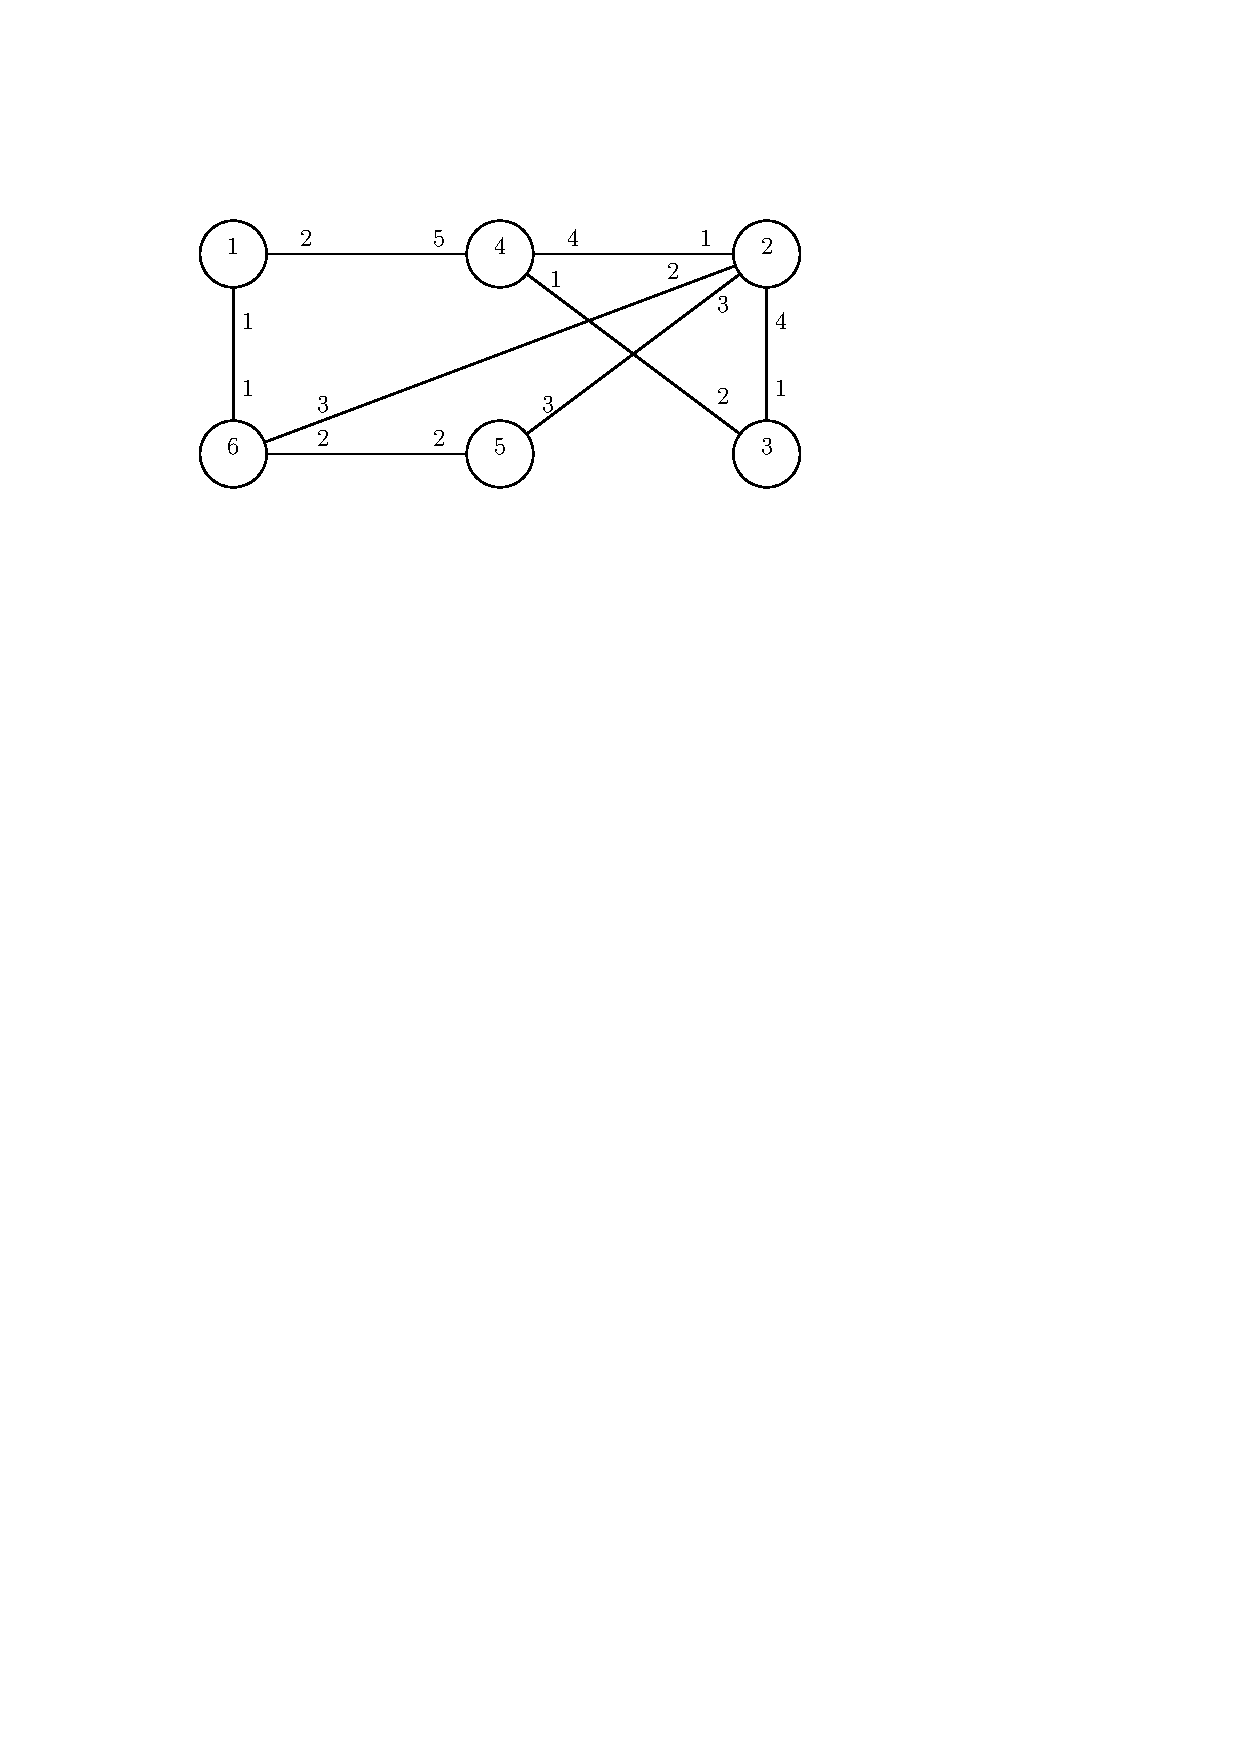
\includegraphics[scale=0.8]{example_graph.pdf}
	\end{figure}
\end{frame}

\begin{frame}{}
	Ogni nodo ha una \textbf{funzione di routing} $f()$ che, 
	per ogni destinazione $v\in V$, specifica il link al quale inviare il messaggio.
	\vfill
	\begin{figure}[h]
	\centering
	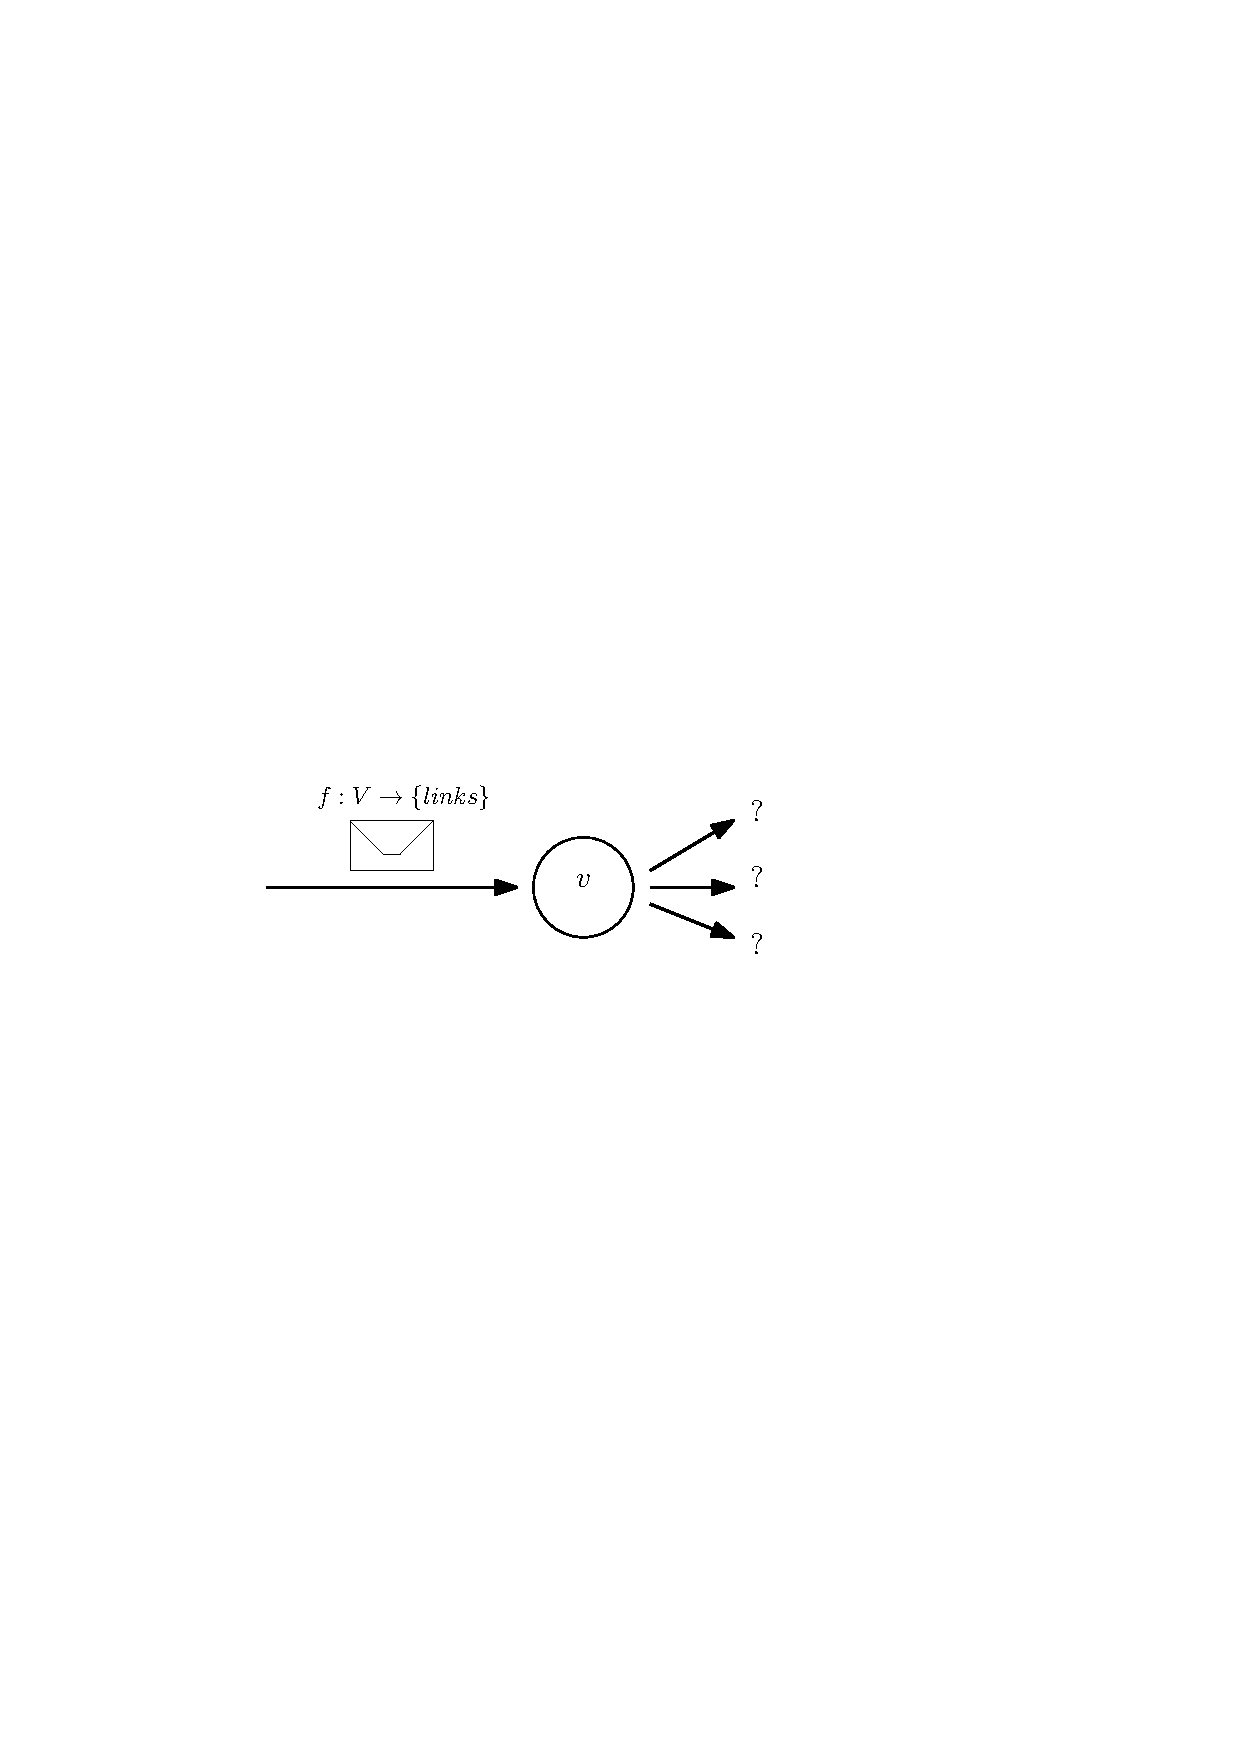
\includegraphics[scale=1]{example_routing.pdf}
	\end{figure}
\end{frame}

\begin{frame}
	\frametitle{Efficienza della funzione di routing}

	\textbf{Routing memory}: bits necessari a memorizzare la funzione di routing $f$.
	\vspace{8pt} 

	\textbf{Search time}: tempo necessario a valutare la funzione di routing $f$ \\(i.e. capire quale link usare).

	\vfill

	\textbf{Tabella di routing}: quando gli arriva un messaggio, il router consulta una tabella locale e determina
	la prossima destinazione del messaggio (cioè la porta sulla quale inoltrarlo).
\end{frame}

\begin{frame}
	\frametitle{}
	
	\textbf{Tabella di routing}: quando gli arriva un messaggio, il router consulta una tabella locale e determina
	la prossima destinazione del messaggio (cioè la porta sulla quale inoltrarlo).

	\vfill
	\begin{figure}[h]
	\centering
	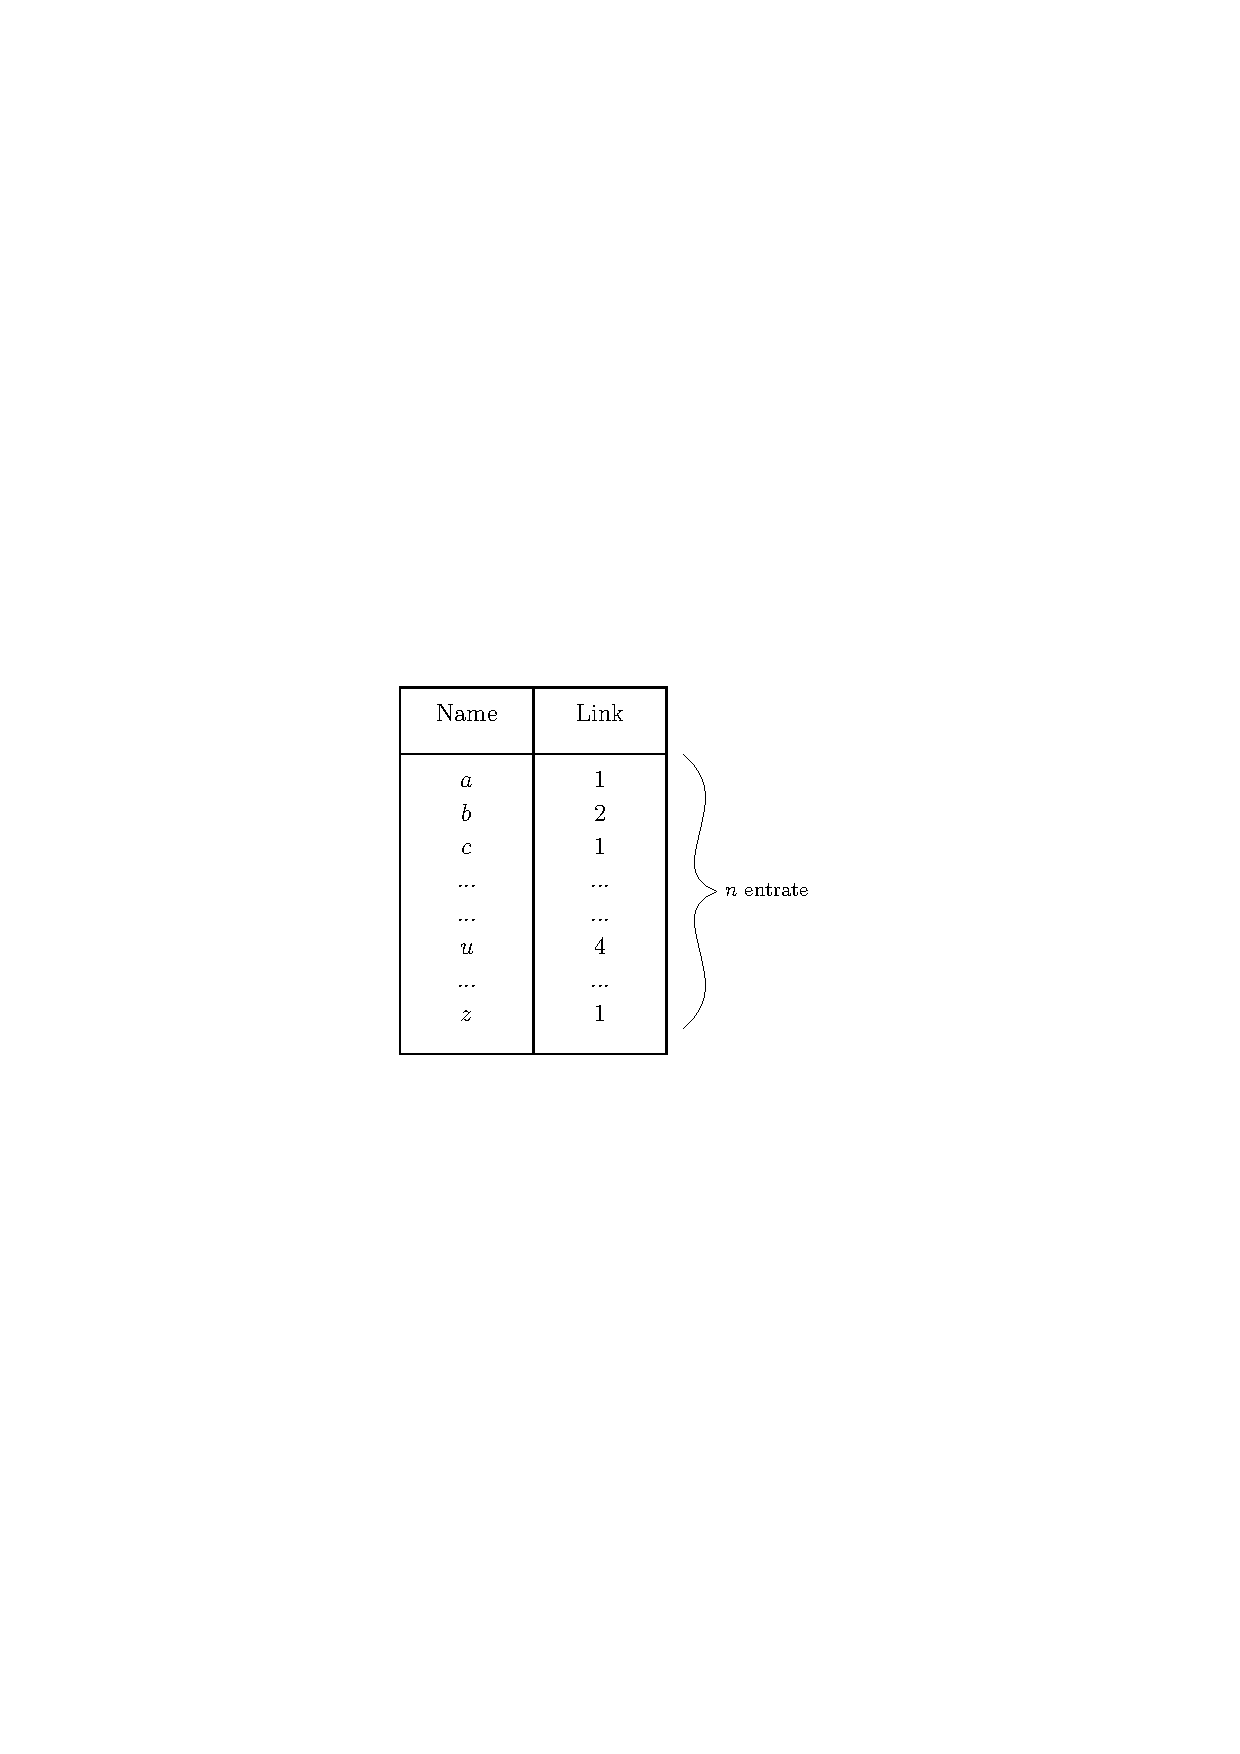
\includegraphics[scale=0.8]{routing_table.pdf}
	\end{figure}
\end{frame}

\begin{frame}
	\frametitle{}
	
	\begin{figure}[h]
	\centering
	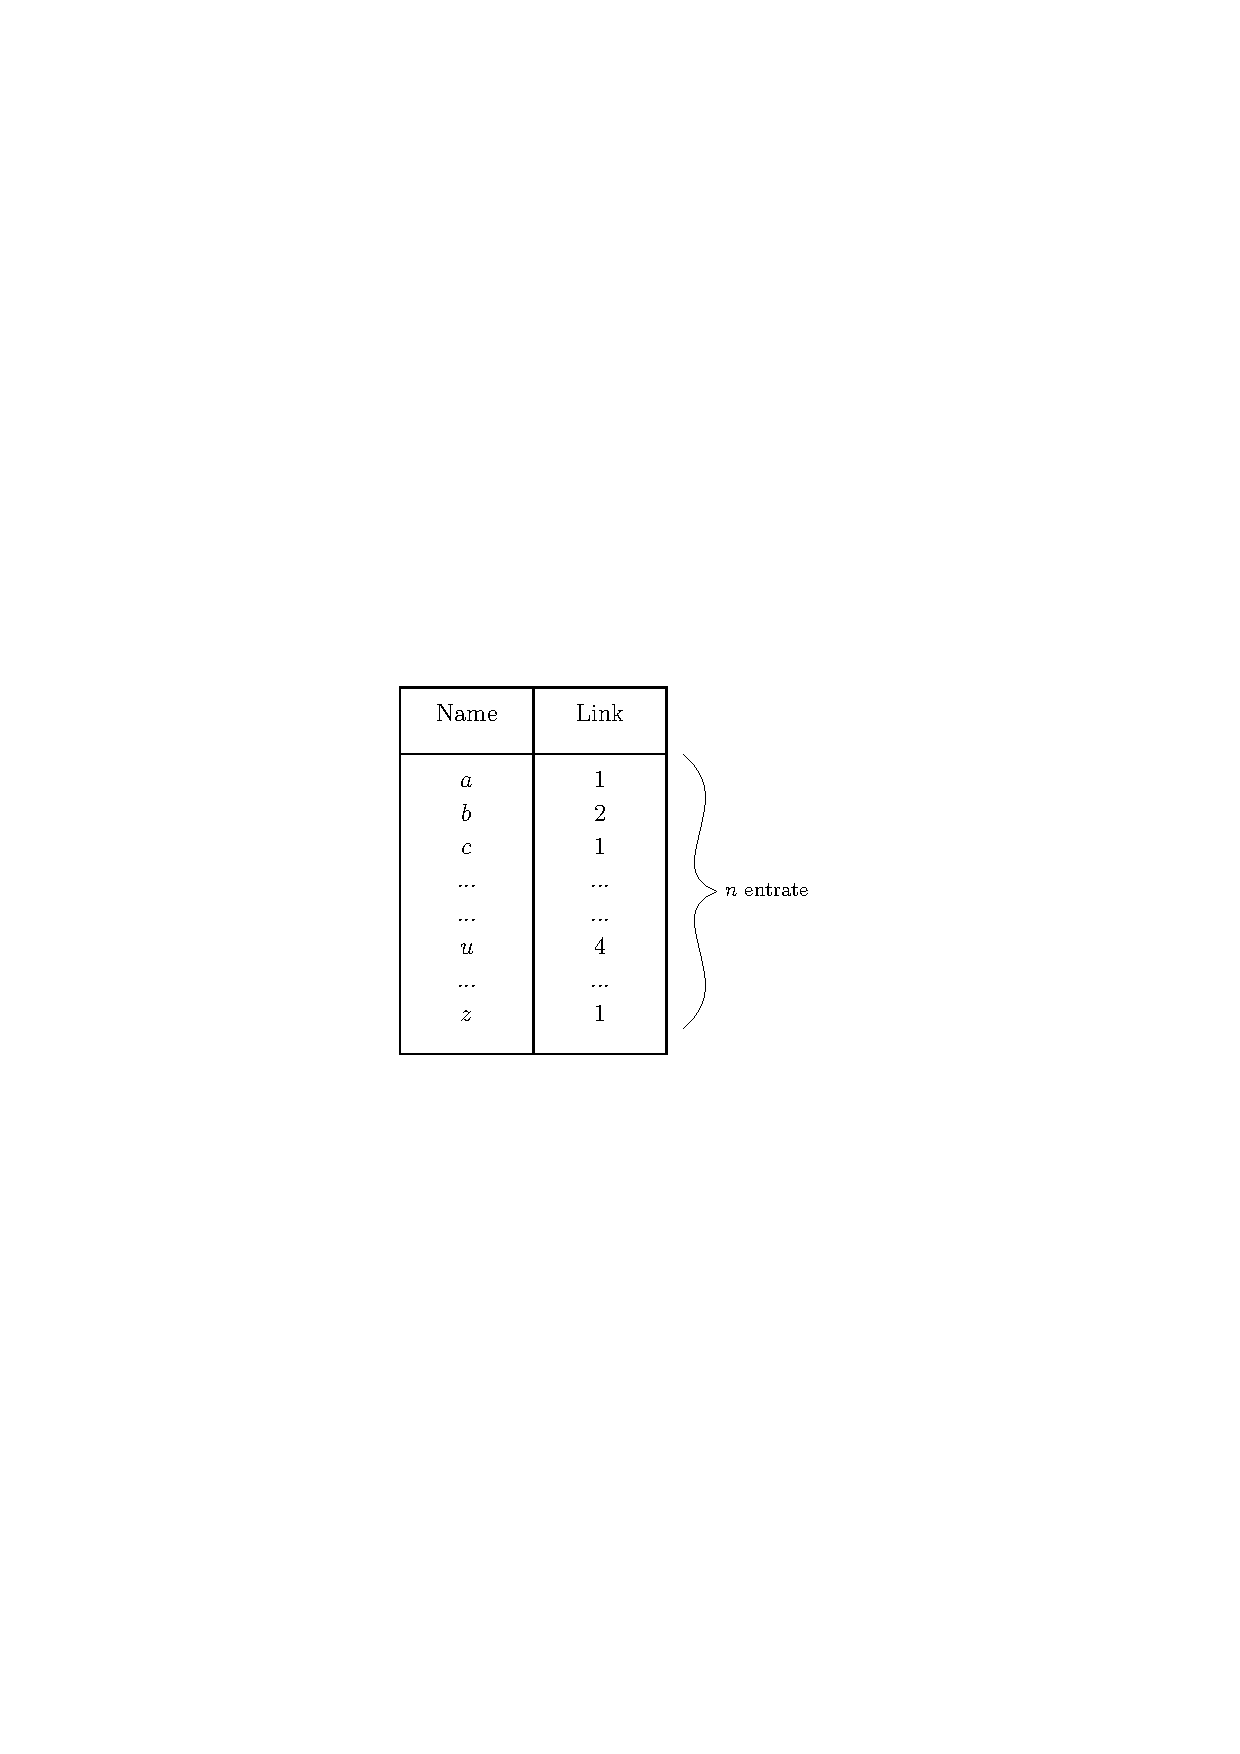
\includegraphics[scale=0.8]{routing_table.pdf}
	\end{figure}

	\vfill 
	\begin{block}{Complessità della tabella di routing}
		\textbf{Routing memory}: $O(n\log n)$\\
		\textbf{Search time}: $O(\log n)$
	\end{block}
\end{frame}

\begin{frame}
	\frametitle{Tabella di routing locale}
	
	\begin{figure}[h]
	\centering
		\begin{subfigure}[b]{0.35\textwidth}
		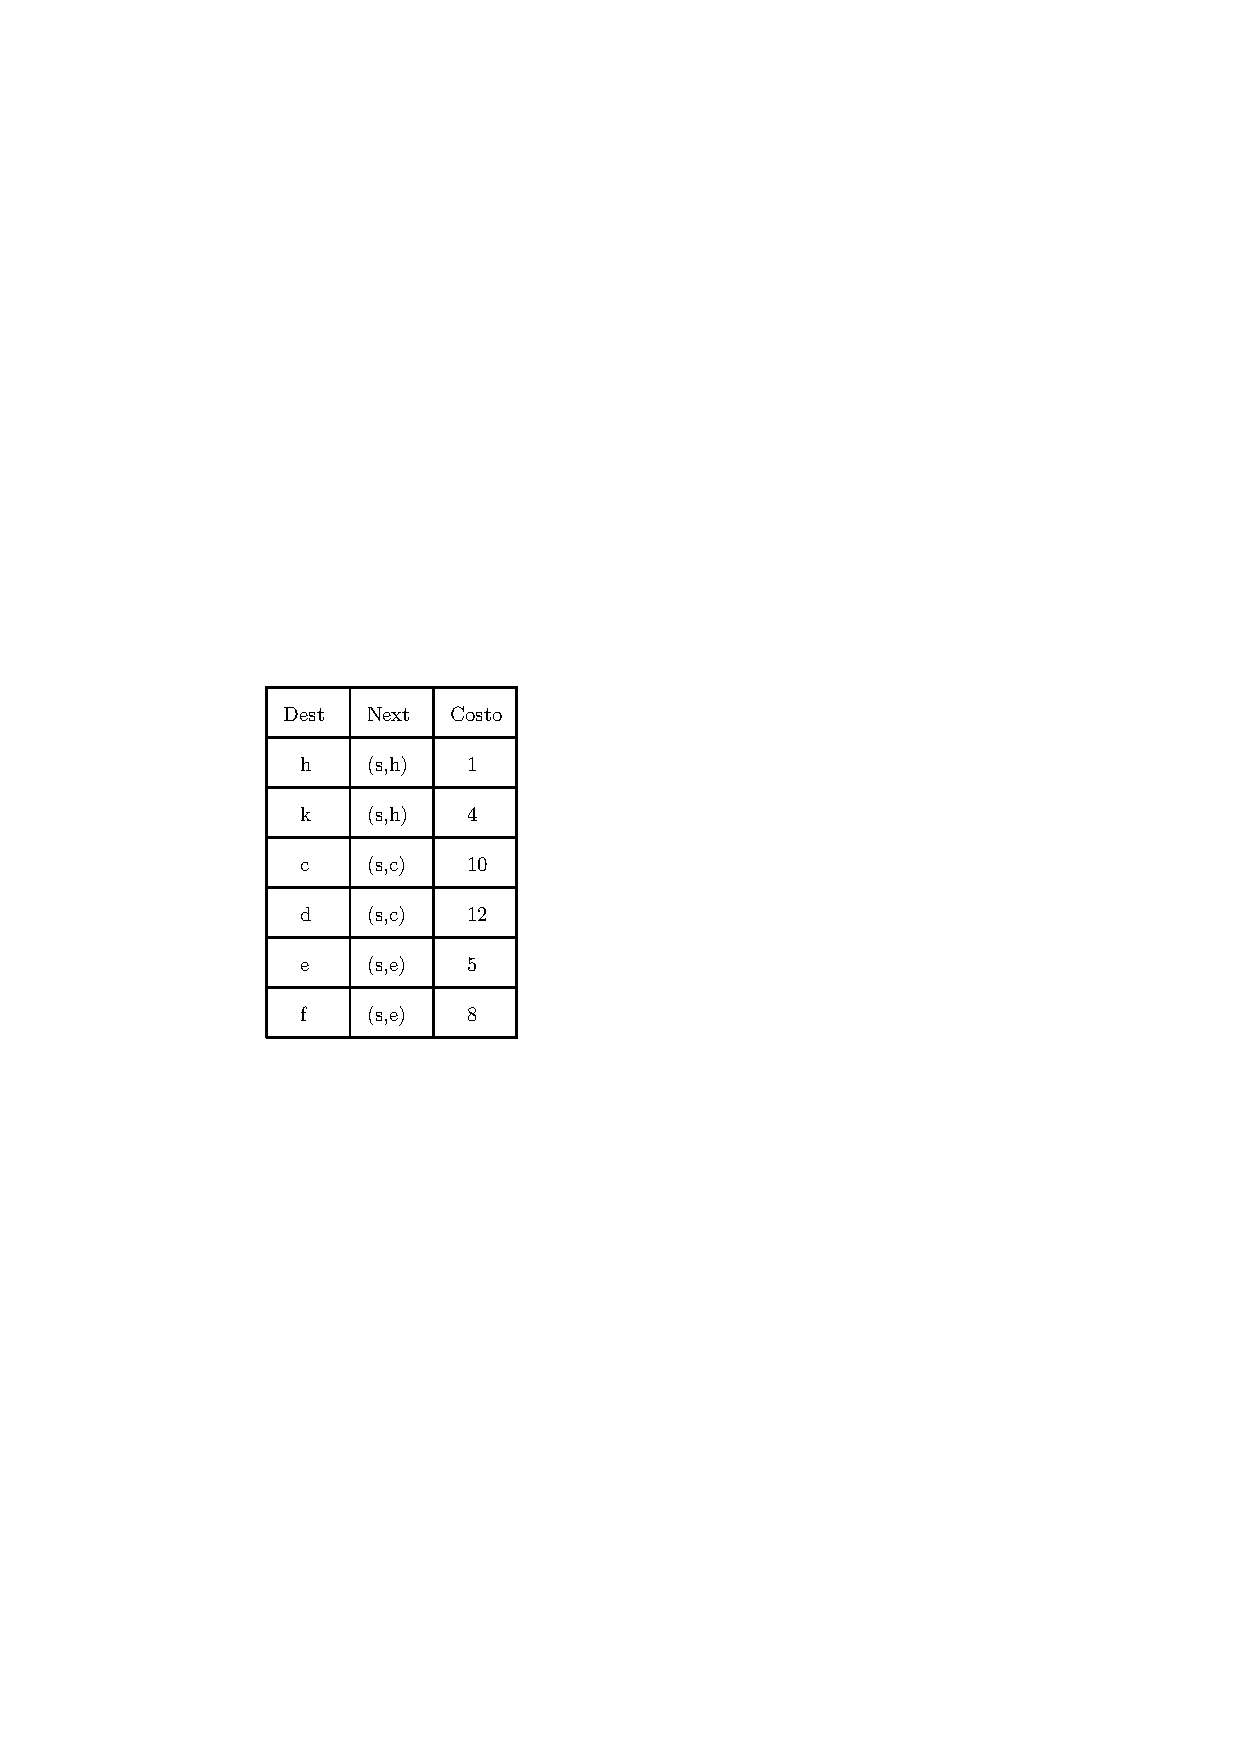
\includegraphics[scale=0.8]{routing_table_local.pdf}
		\end{subfigure}
		\begin{subfigure}[b]{0.6\textwidth}
		\hspace*{22pt}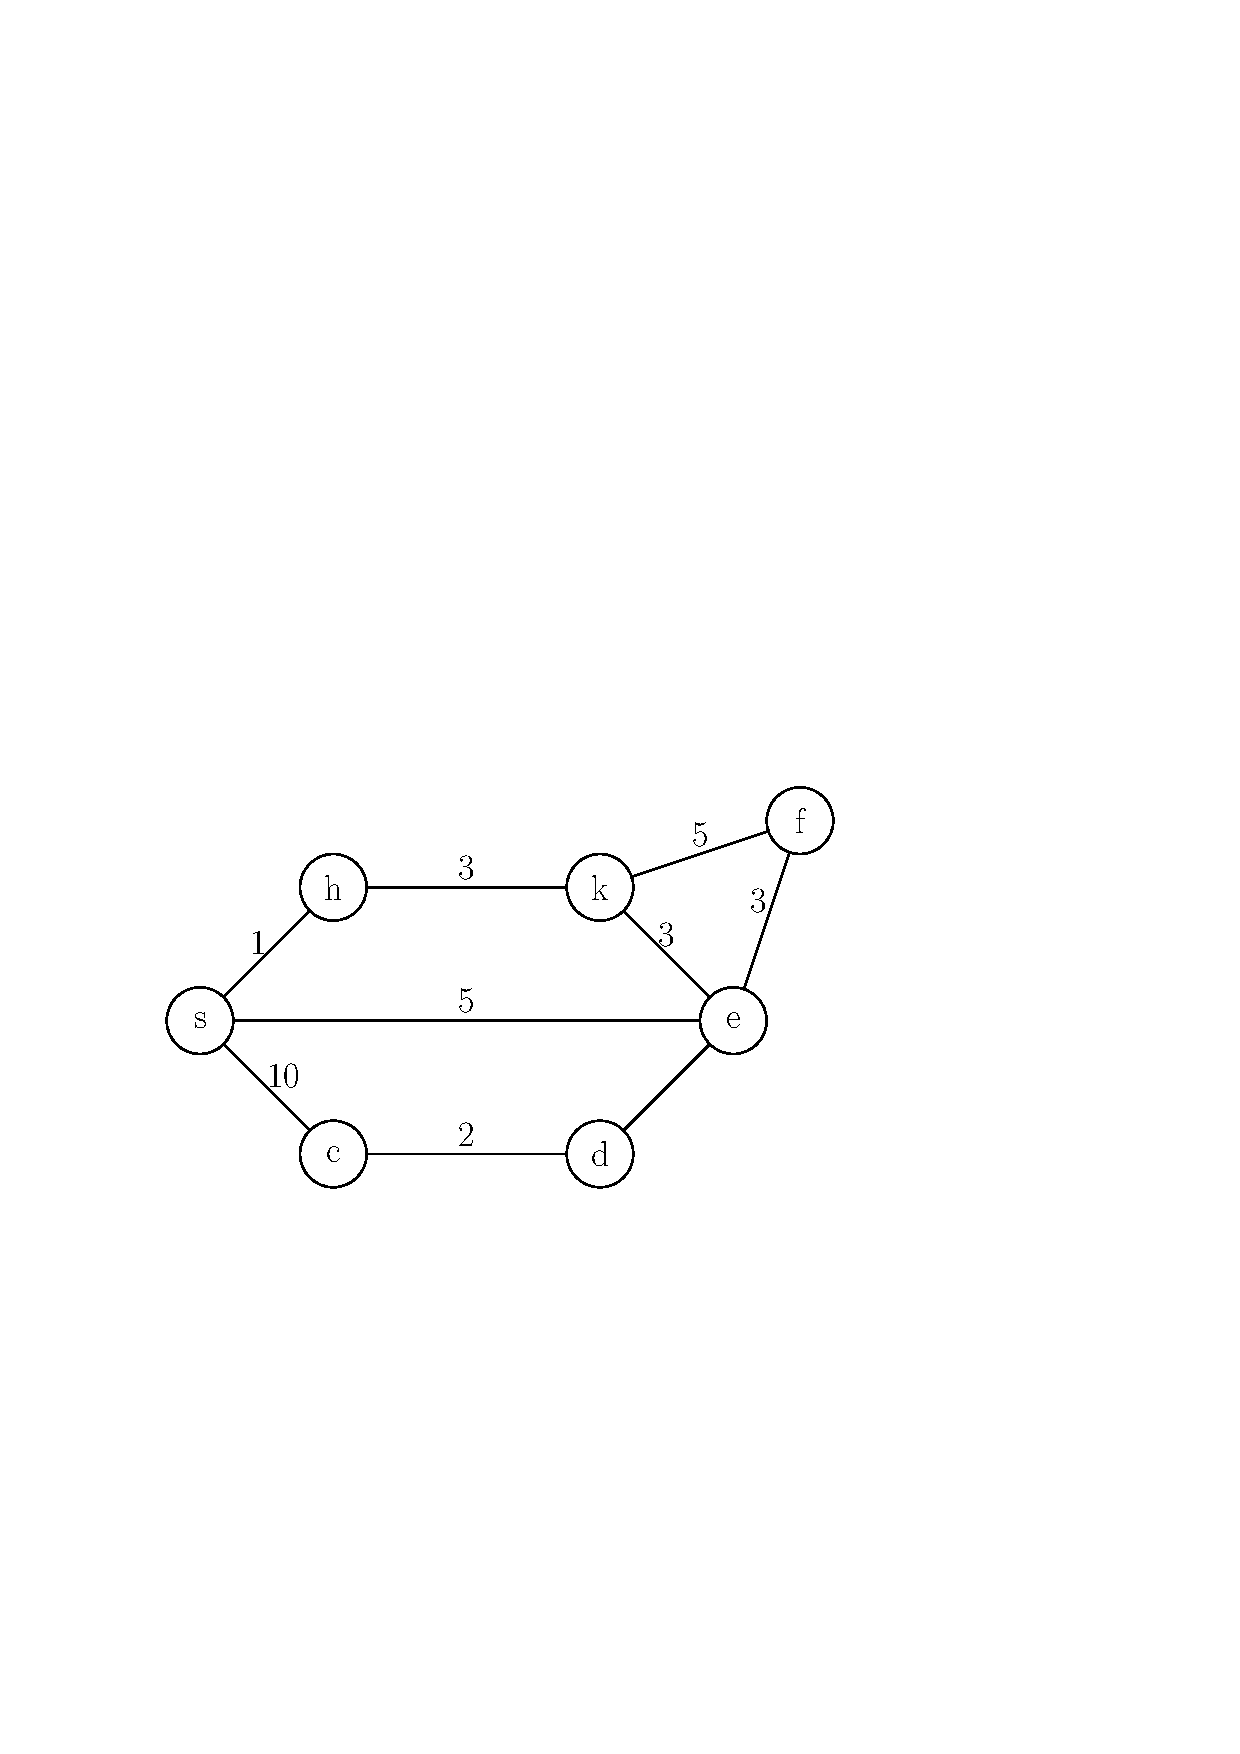
\includegraphics[width=.85\linewidth]{routing_table_graph.pdf}
		\end{subfigure}
	\end{figure}
\end{frame}

\begin{frame}
	\frametitle{Tabella di routing globale}
	
	\begin{figure}[h]
	\centering
		\begin{subfigure}[b]{0.35\textwidth}
		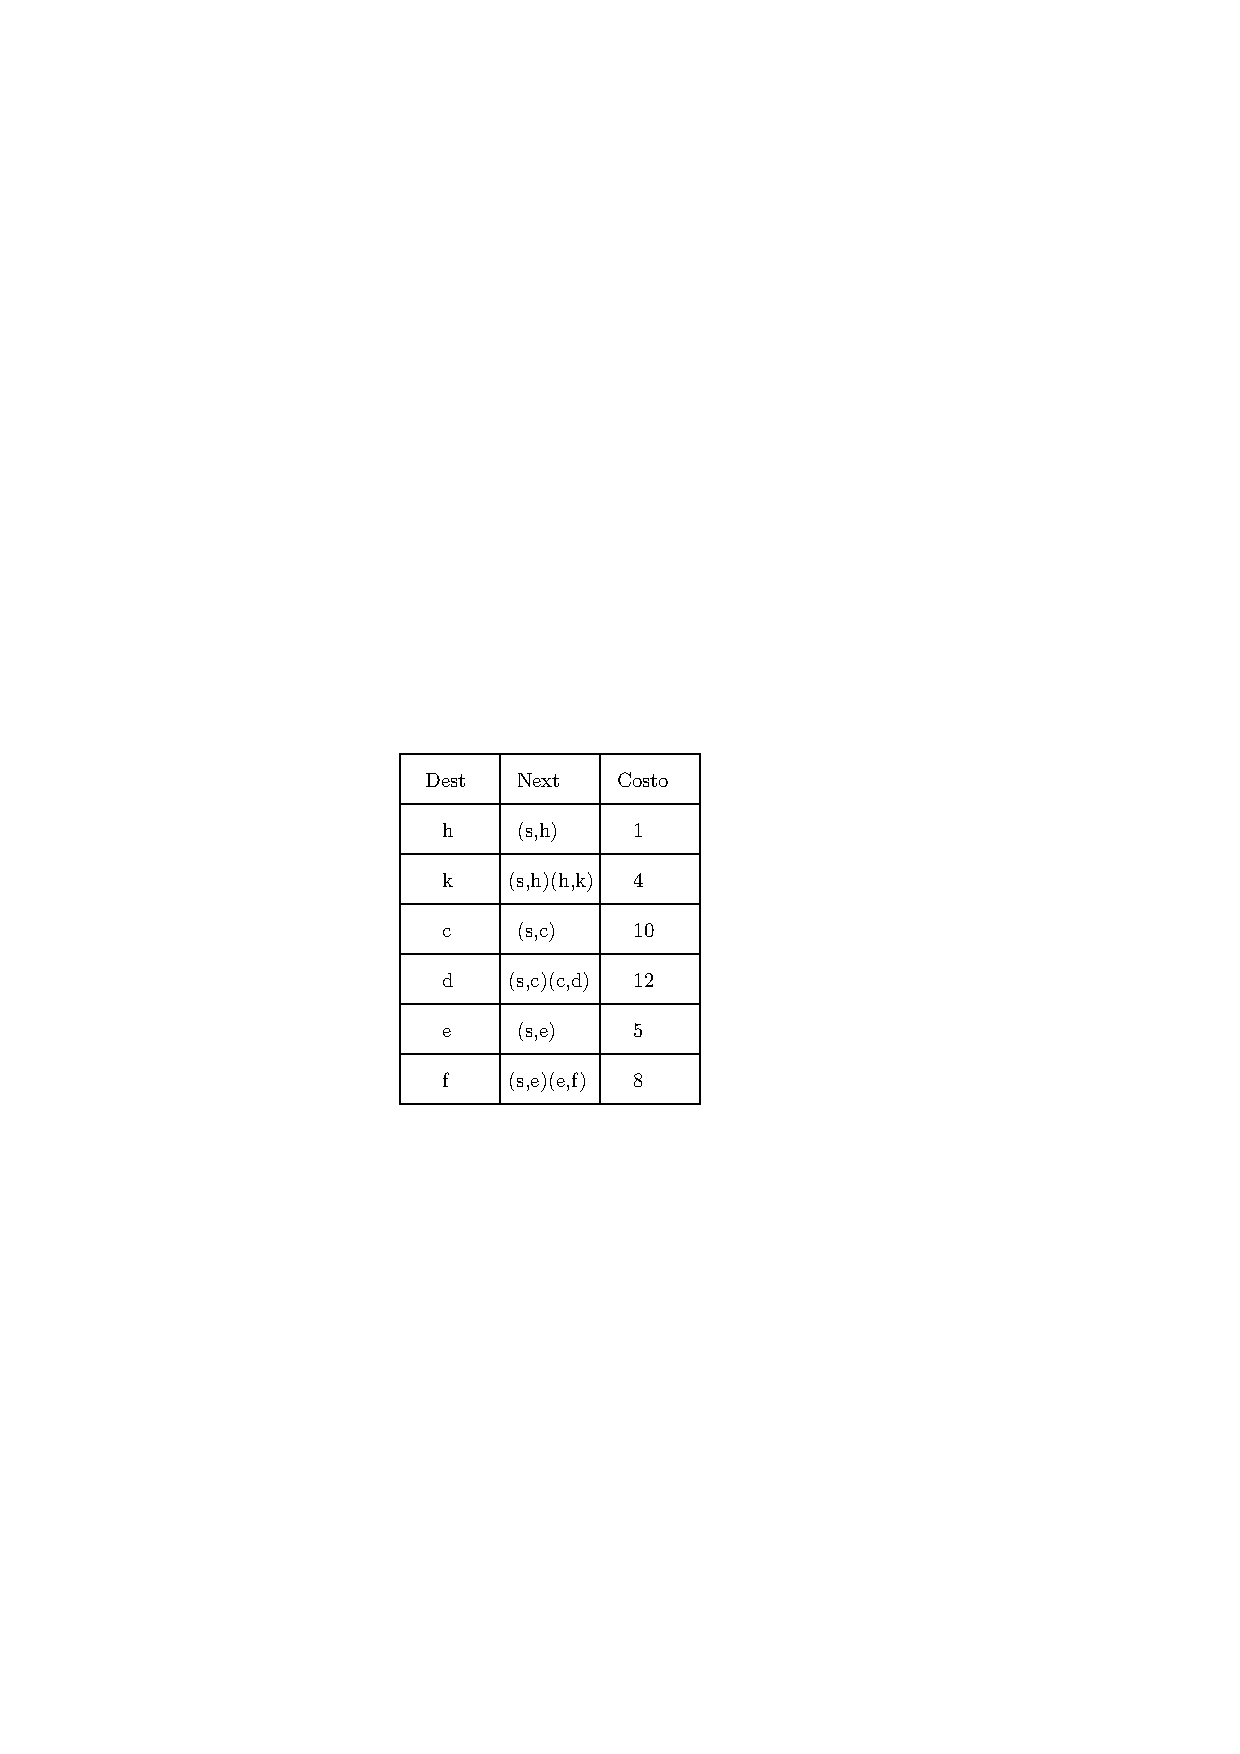
\includegraphics[scale=0.8]{routing_table_global.pdf}
		\end{subfigure}
		\begin{subfigure}[b]{0.6\textwidth}
		\hspace*{22pt}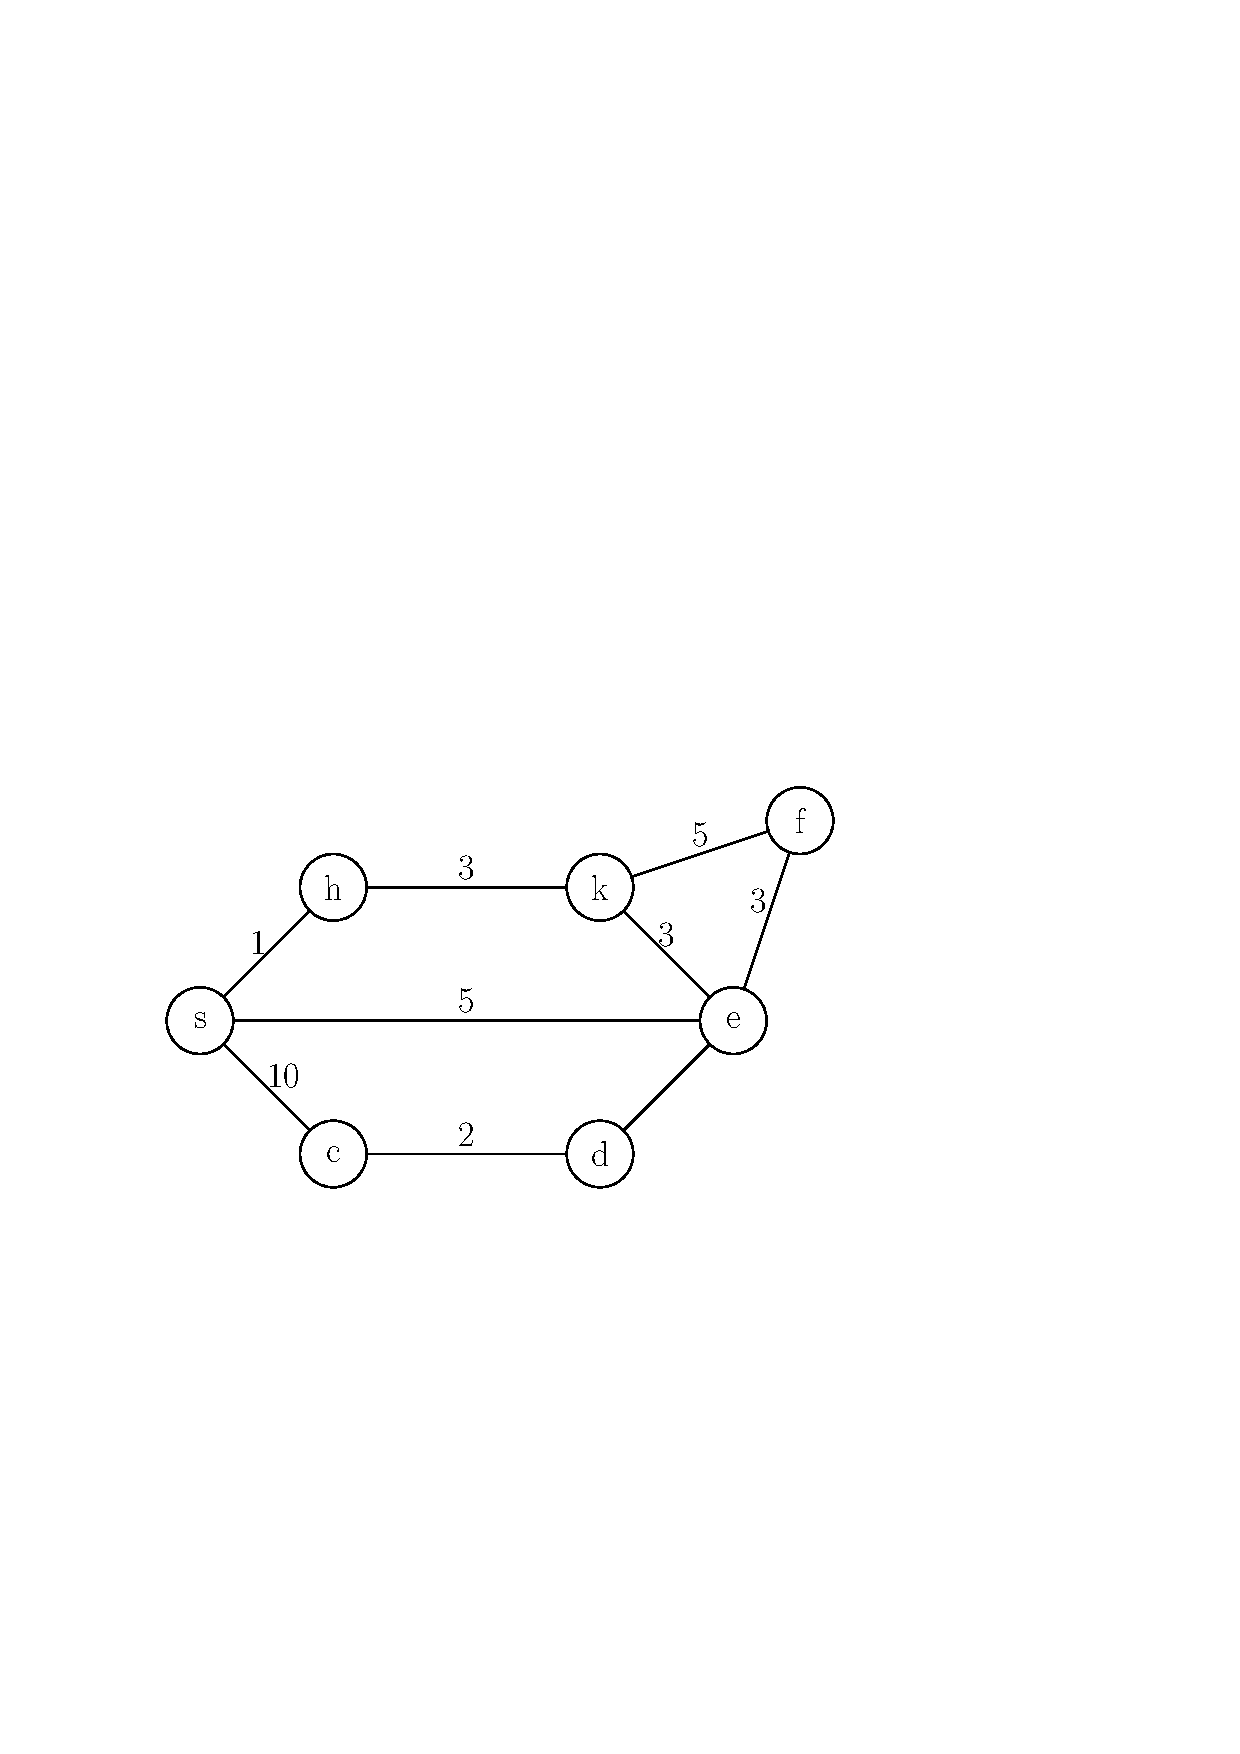
\includegraphics[width=.85\linewidth]{routing_table_graph.pdf}
		\end{subfigure}
	\end{figure}
\end{frame}

\begin{frame}
	\frametitle{Algoritmo Map-Gossip}
	Per costruire \textbf{tutte} le tabelle di routing
	ogni nodo fa il broadcast delle sue informazioni iniziali.

	\vfill
	\begin{block}
		{Map-Gossip}
		\begin{itemize}
			\item Crea uno spanning tree arbitrario.
			\item Ogni nodo colleziona le informazioni dei suoi vicini.
			\item Ogni nodo diffonde (broadcast) le proprie informazioni lungo l'albero.
		\end{itemize}
	\end{block}
\end{frame}

\begin{frame}
	\frametitle{Message Complexity di Map-Gossip}
	
	\pause
	 Crea uno spanning tree arbitrario: $O(m+\log n)$\\
	   (e.g. con Mega-Merger)
	\vfill

	\pause
	 Ogni nodo colleziona le informazioni dei suoi vicini: $2m$
	\vfill

	\pause
	 Ogni nodo diffonde (broadcast) le proprie informazioni lungo l'albero:
	   $$ \sum_x deg(x)(n-1)=2m(n-1)$$
	\vfill

	\pause
	Totale: $O(mn)$
	\pause
	\\
	\textcolor{red}{Warning}: I messaggi sono \textbf{grandi}!
	\\Osservazione: un nodo deve avere abbastanza spazio per immagazzinare la tabella di routing.
		
\end{frame}

\begin{frame}
	\frametitle{Costruzione iterativa delle tabelle di routing}
	Supponiamo che i nodi non abbiano abbastanza spazio per immagazzinare l'intera tabella di routing.
	\vfill
	\pause

	Inizialmente un nodo conosce solo i suoi vicini.

	\begin{figure}[h]
	\centering
		\begin{subfigure}[b]{0.35\textwidth}
			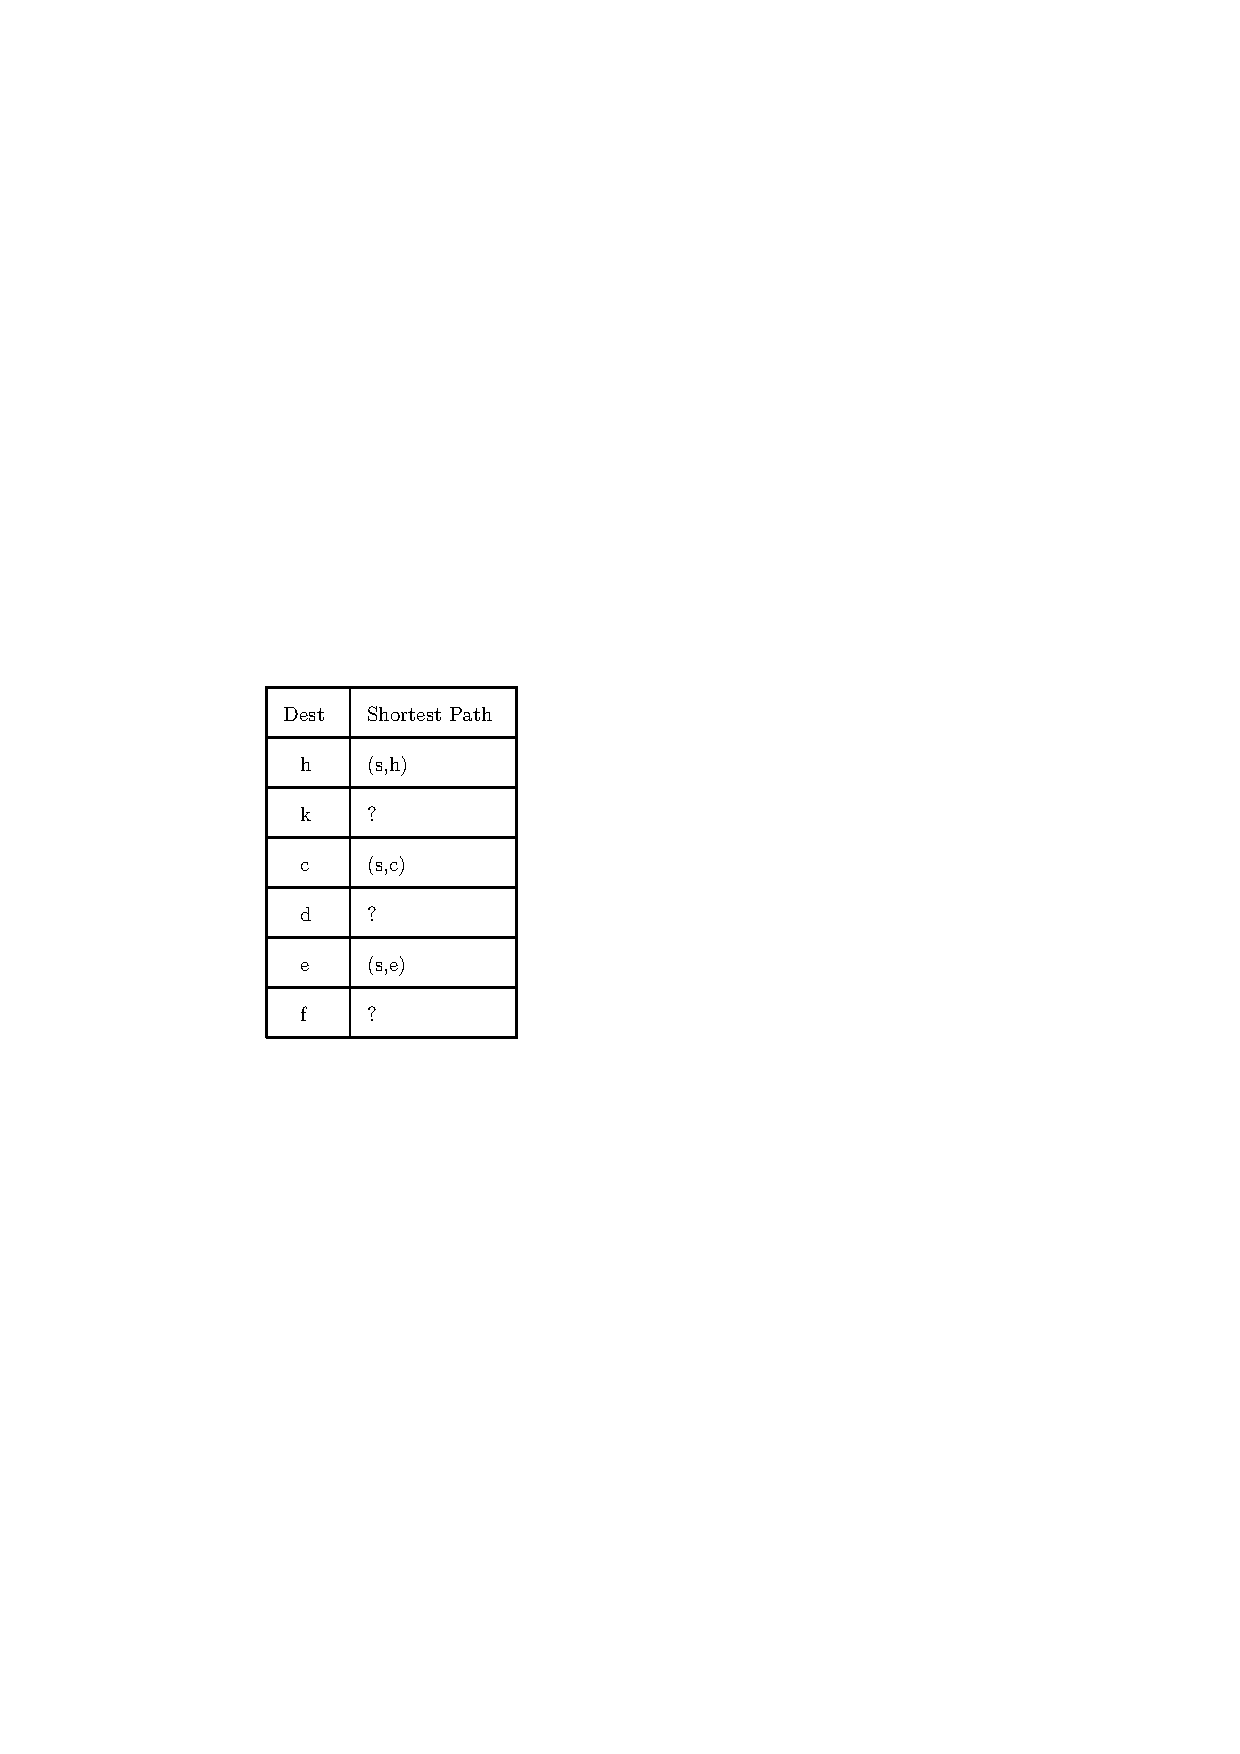
\includegraphics[scale=0.8]{routing_table_local_initial.pdf}
			\caption*{Vettore delle distanze.}
		\end{subfigure}
		\begin{subfigure}[b]{0.6\textwidth}
		\hspace*{22pt}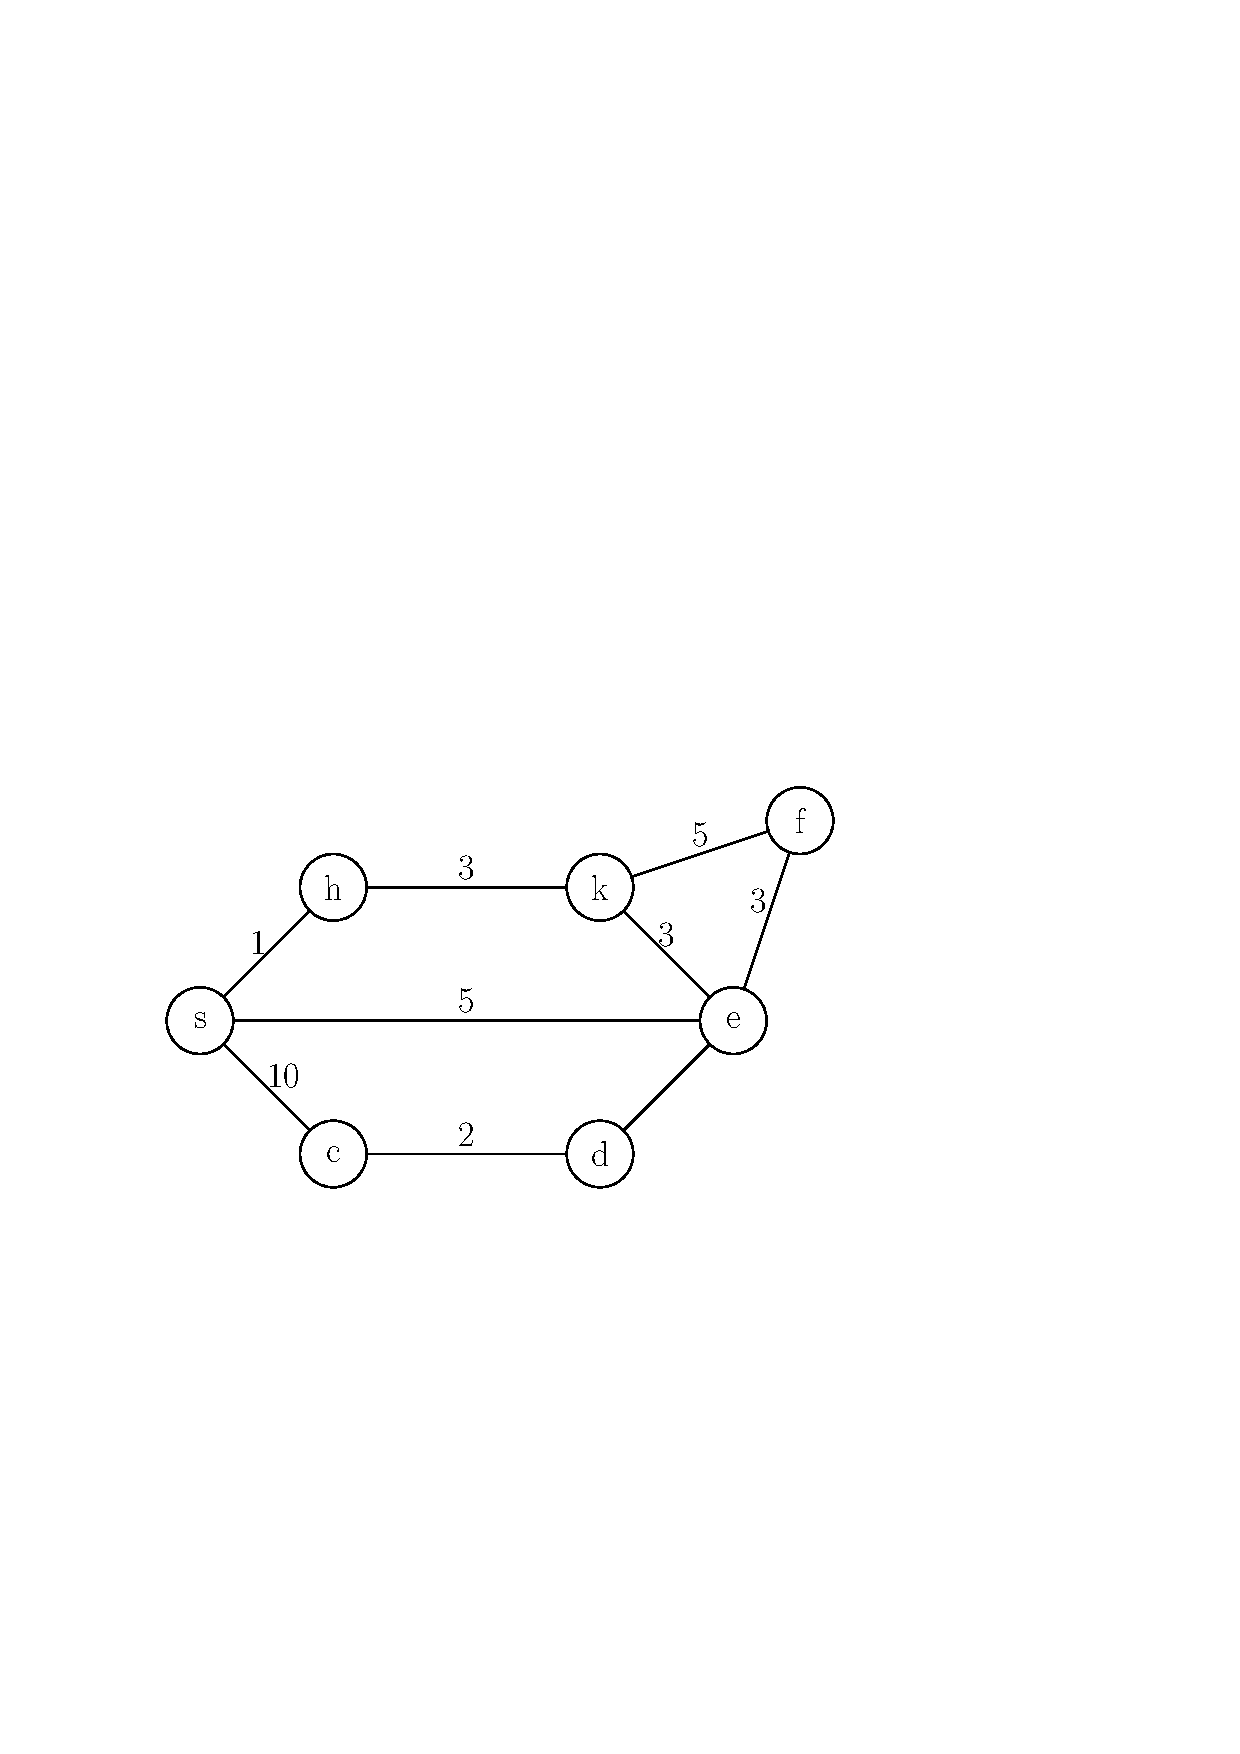
\includegraphics[width=.85\linewidth]{routing_table_graph.pdf}
		\end{subfigure}
	\end{figure}
\end{frame}

\begin{frame}
	\frametitle{}
	Ad ogni iterazione ogni nodo invia il suo vettore delle distanze corrente ai suoi vicini.
	\vfill
	A sua volta, ogni nodo dunque riceve il vettore delle distanze dei suoi vicini, e aggiorna
	il proprio in accordo ad esso.
\end{frame}

\begin{frame}
	\frametitle{}
	
	\begin{figure}[h]
		\hspace*{22pt}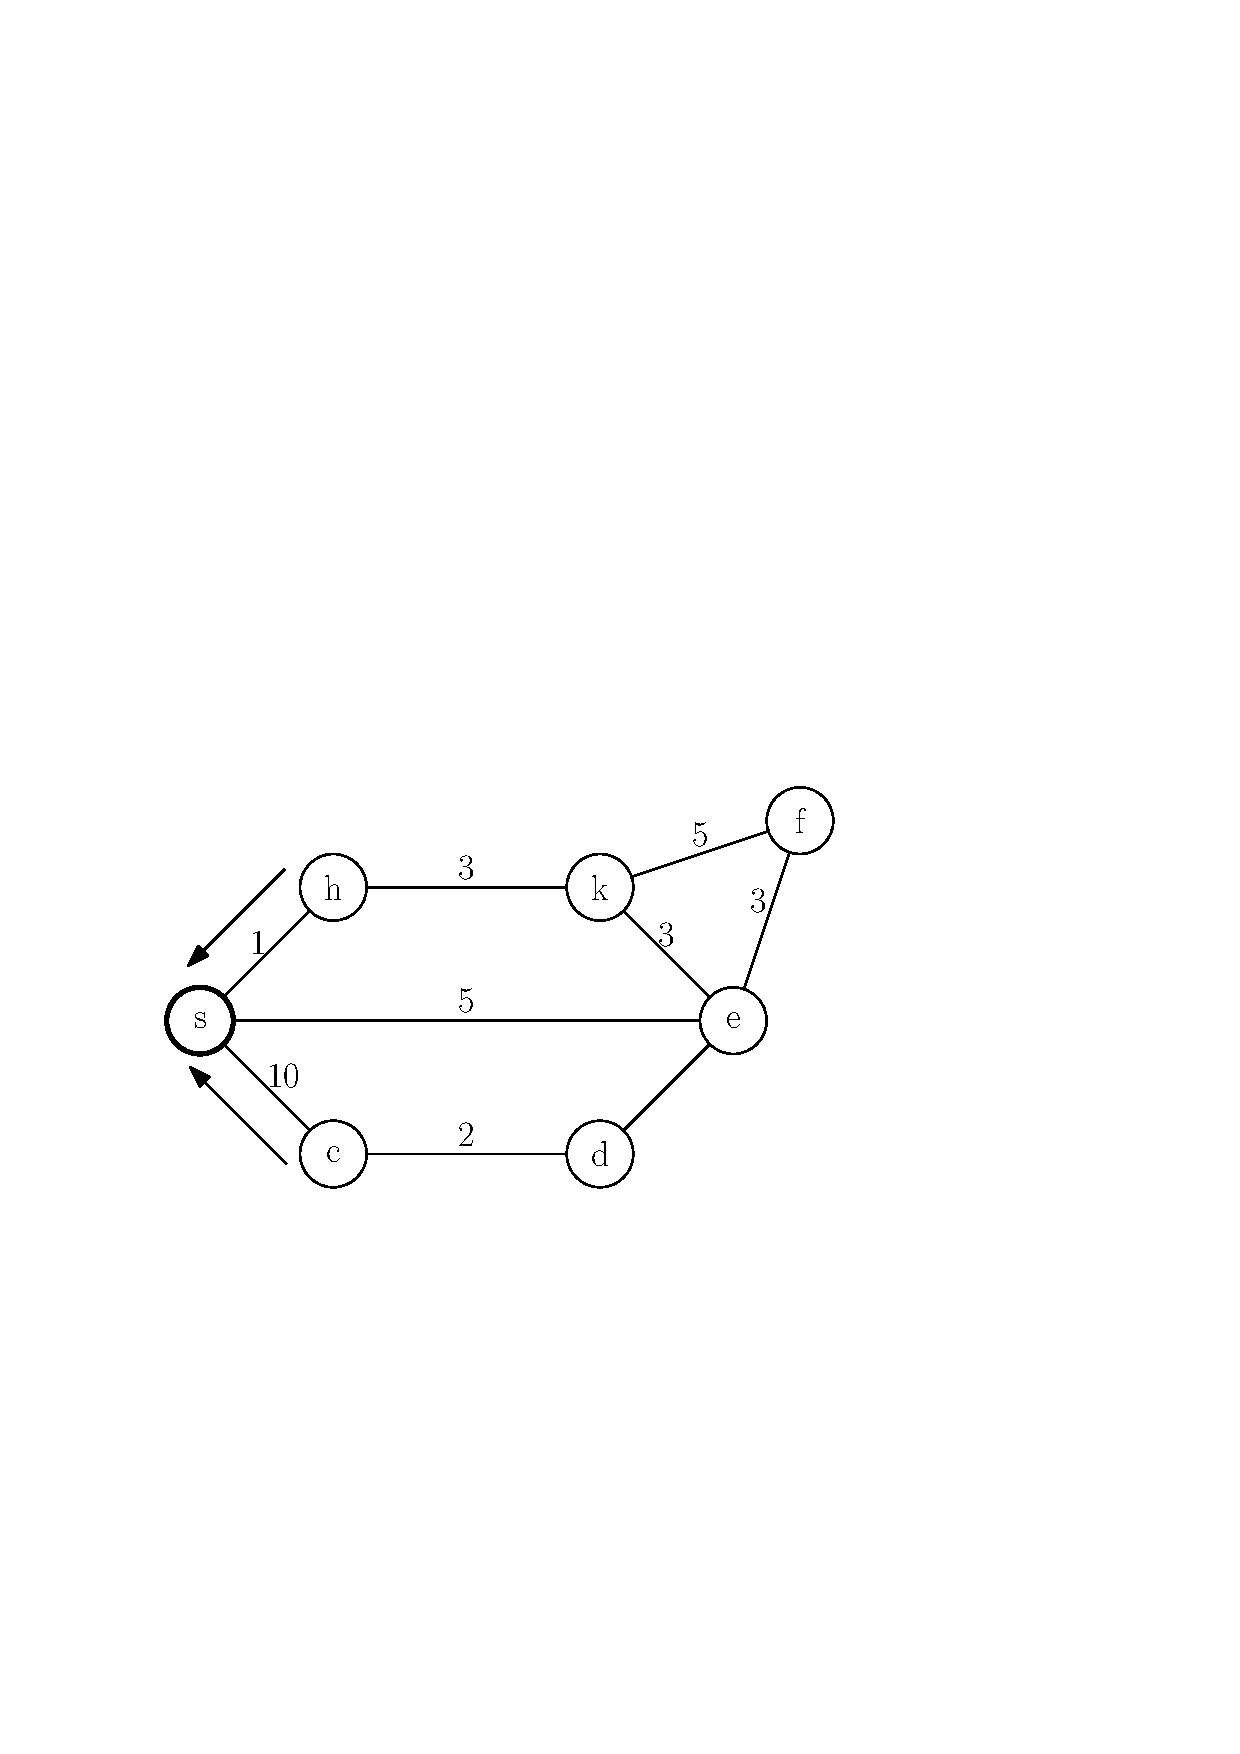
\includegraphics[scale=0.5]{routing_table_graph_send.pdf}
	\end{figure}
	\begin{figure}[h]
	\centering
		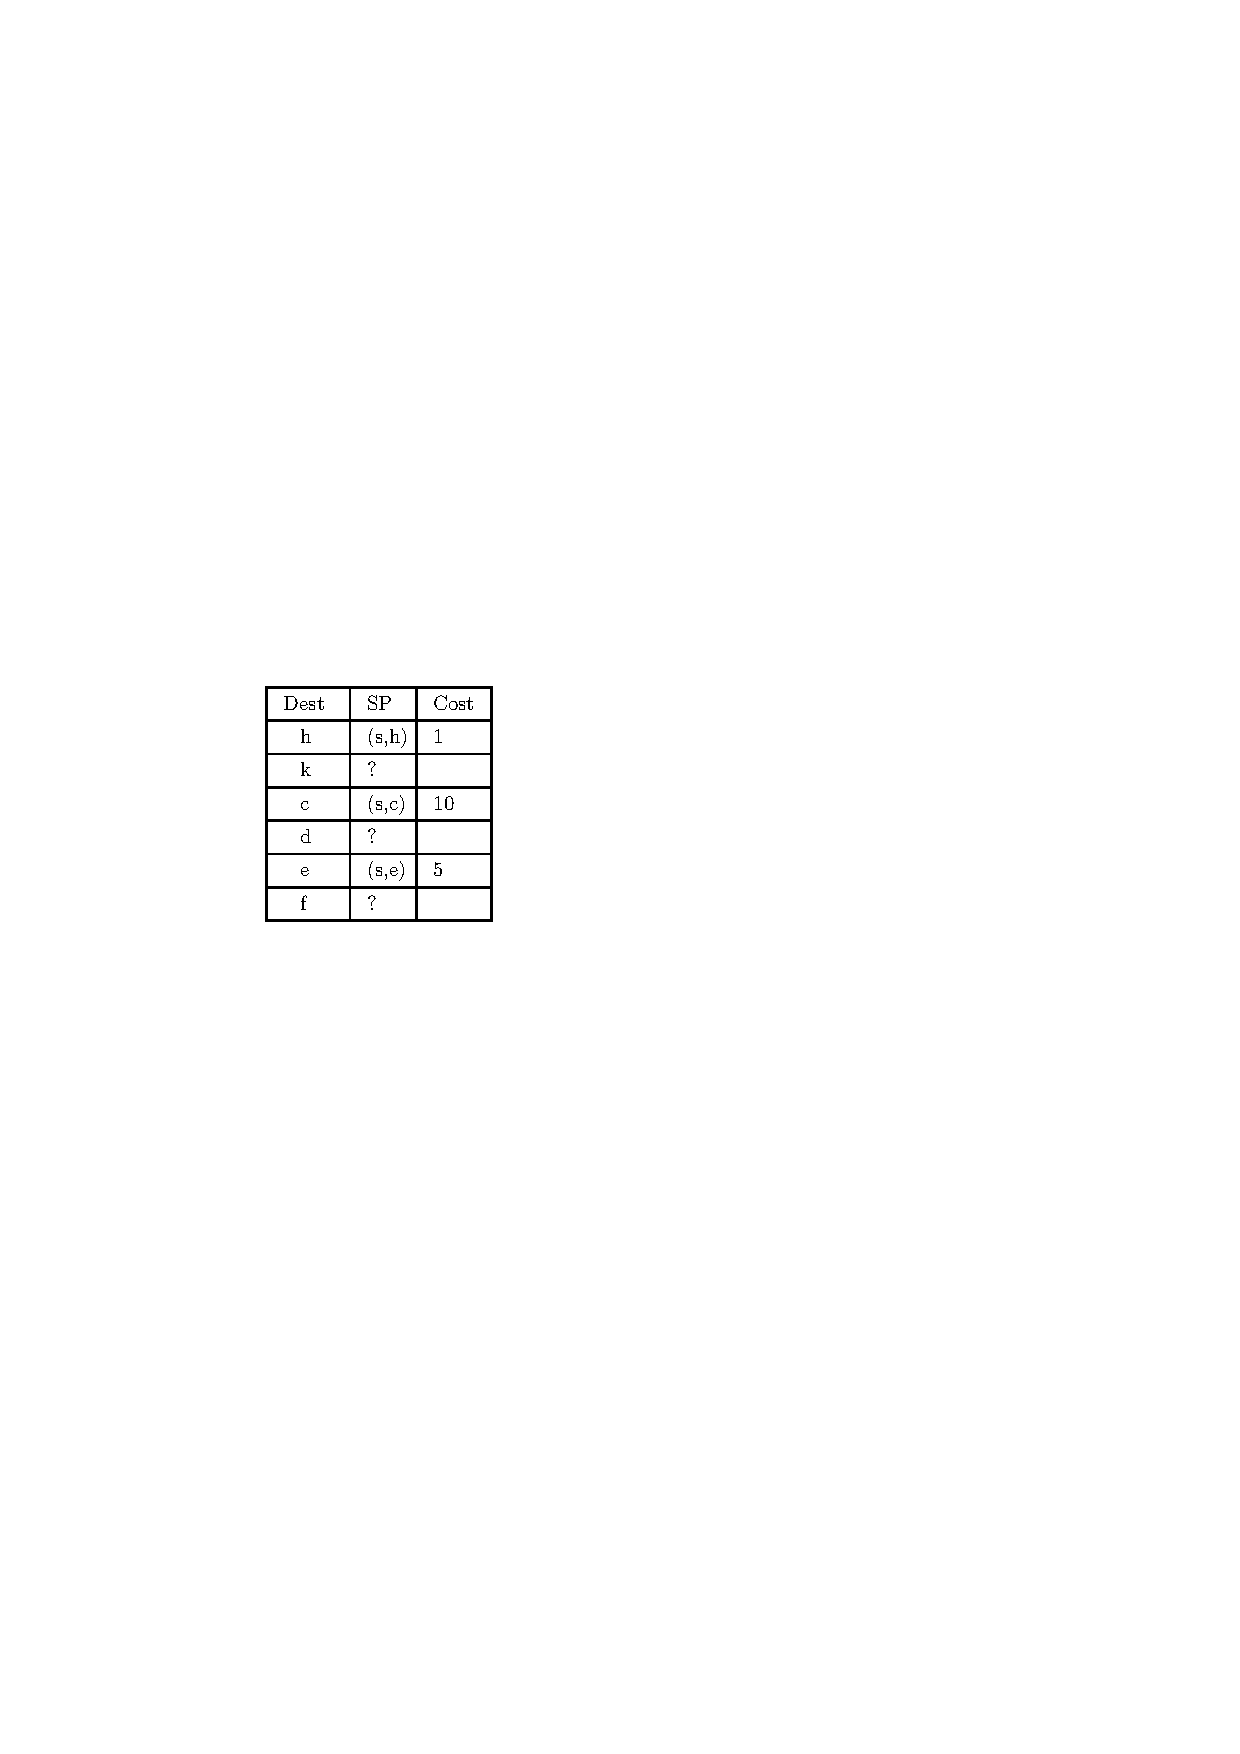
\includegraphics[scale=0.7]{routing_table_local_initial_s.pdf}
		\caption*{Tabella di $s$.}
	\end{figure}
\end{frame}

\begin{frame}
	\frametitle{}
	
	\begin{figure}[h]
		\hspace*{22pt}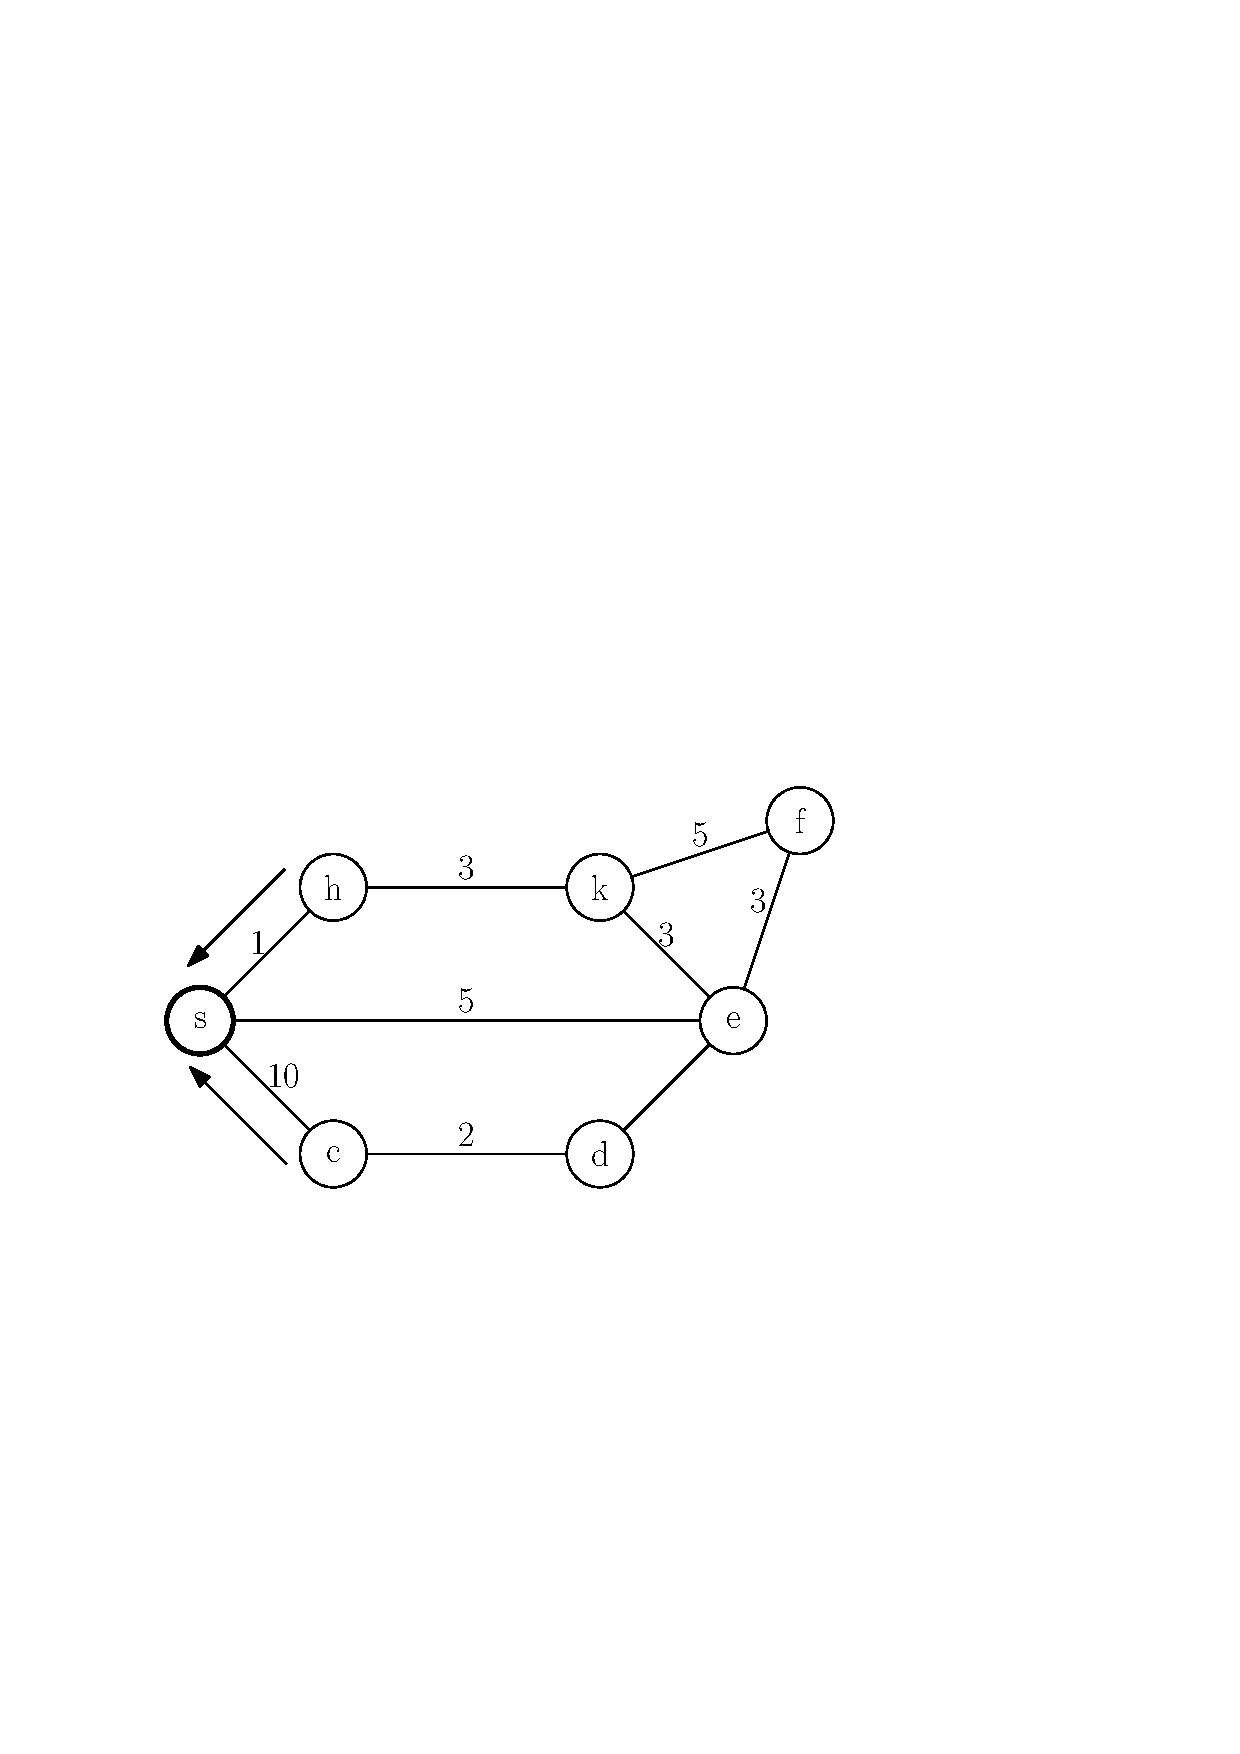
\includegraphics[scale=0.5]{routing_table_graph_send.pdf}
	\end{figure}
	\begin{figure}[h]
	\centering
		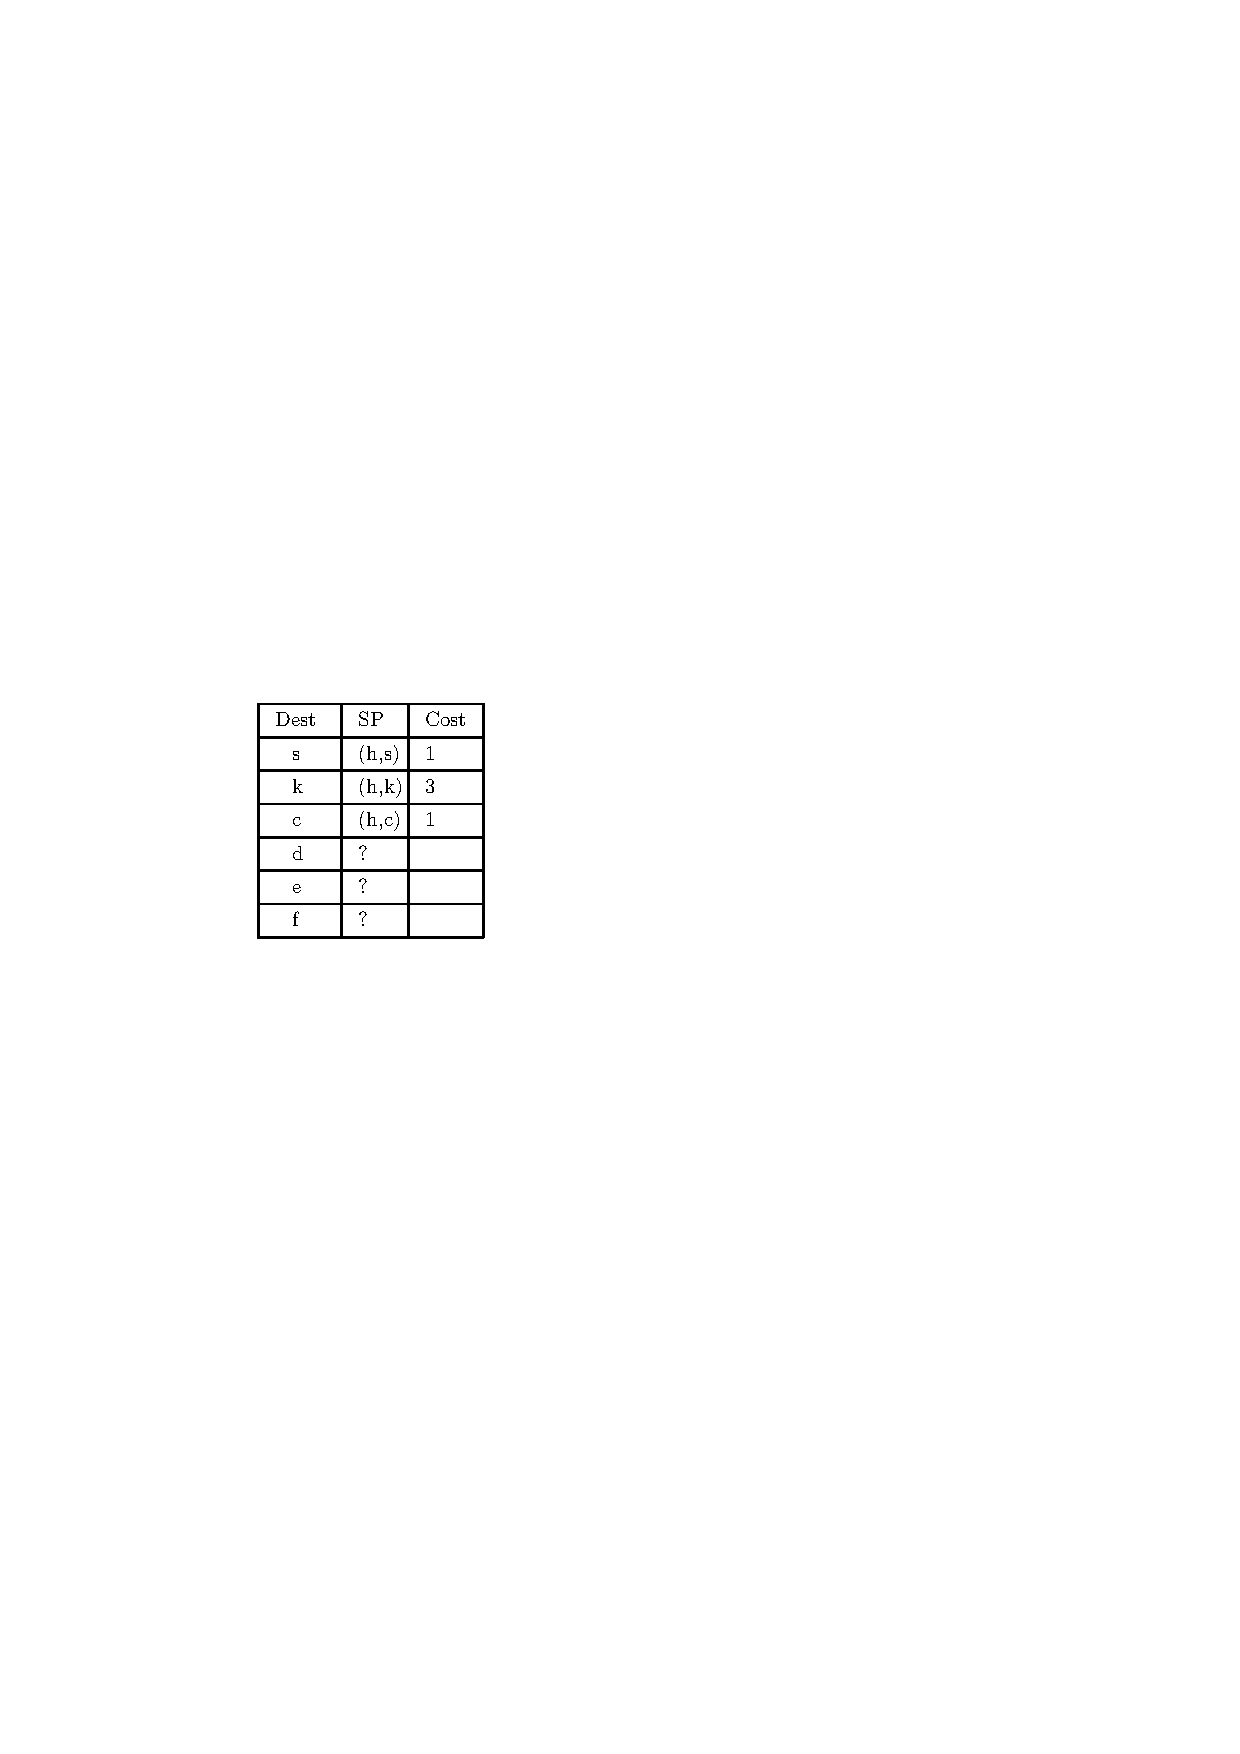
\includegraphics[scale=0.7]{routing_table_local_initial_h.pdf}
		\caption*{Tabella di $h$.}
	\end{figure}
\end{frame}

\begin{frame}
	\frametitle{}
	
	\begin{figure}[h]
		\hspace*{22pt}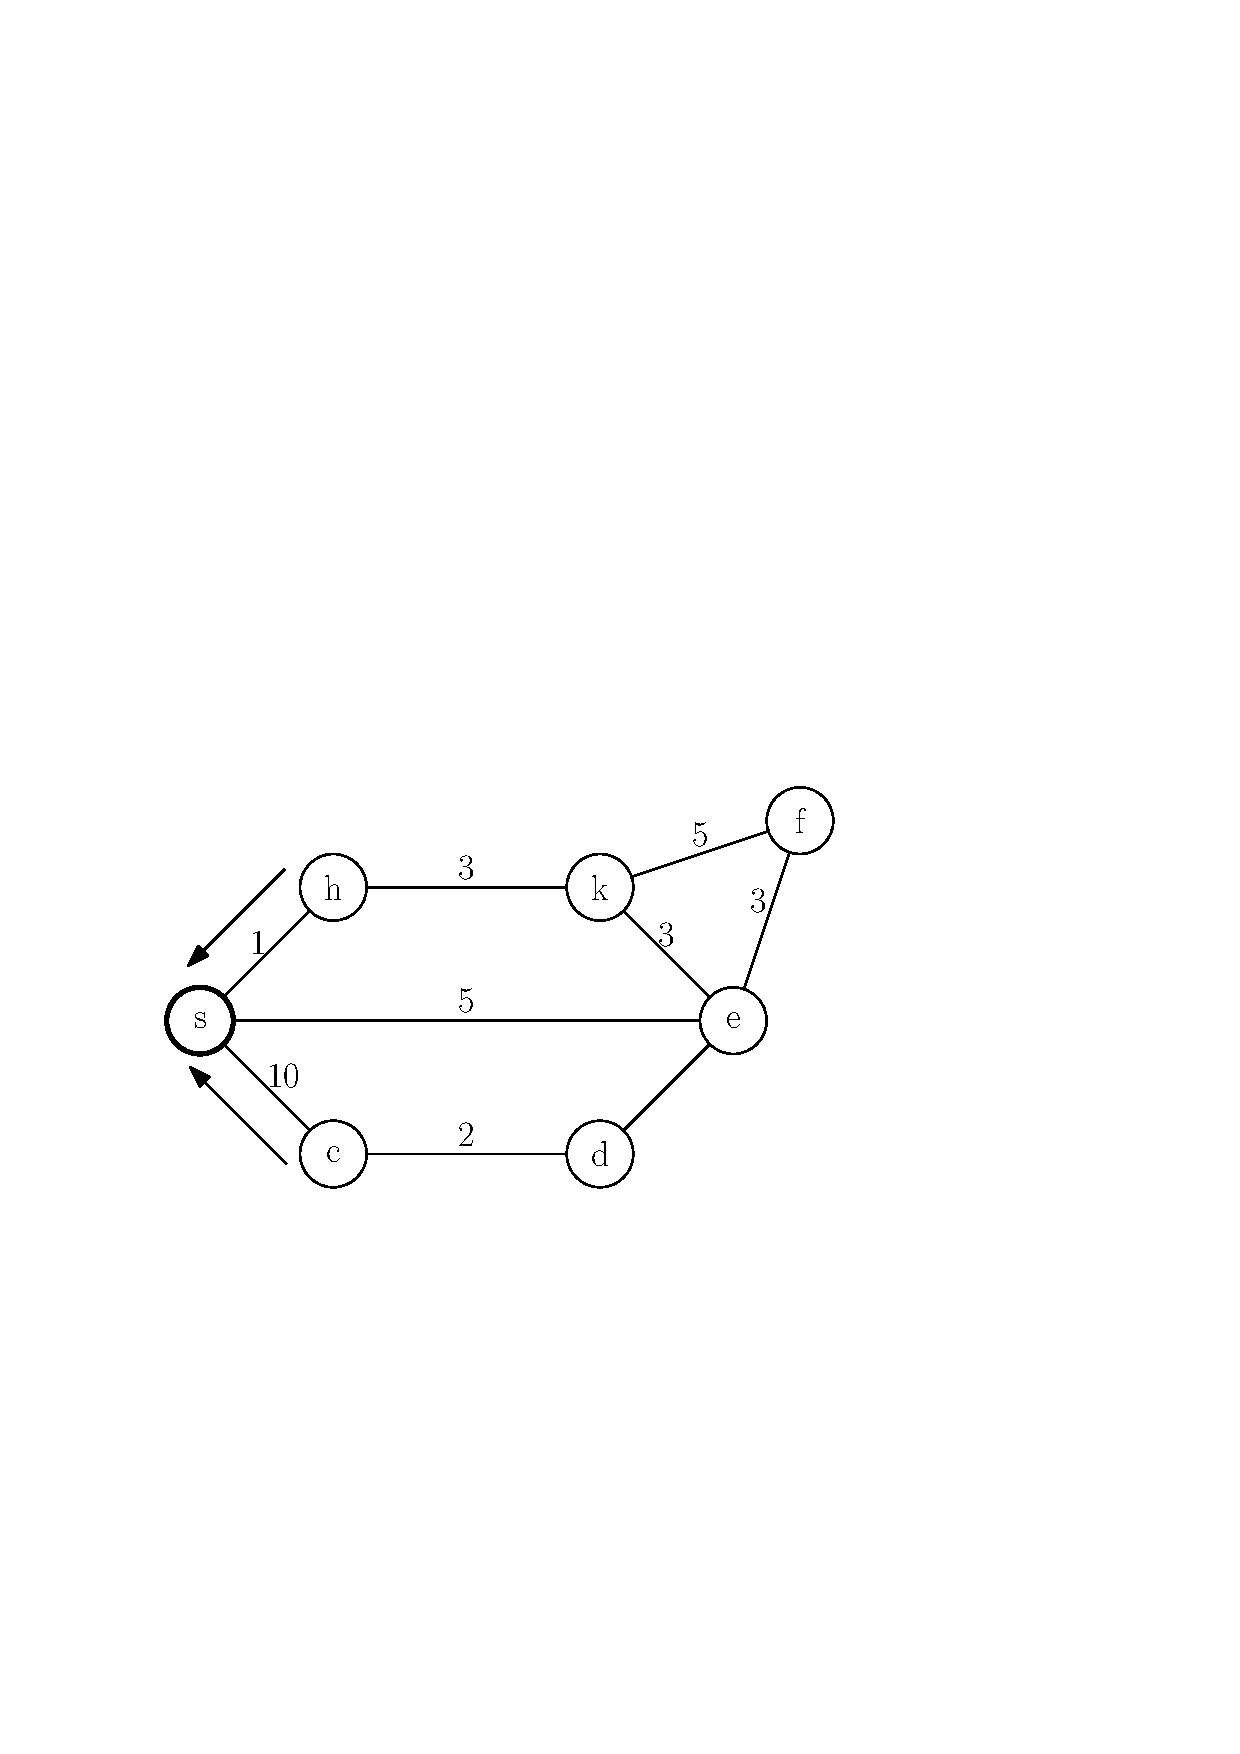
\includegraphics[scale=0.5]{routing_table_graph_send.pdf}
	\end{figure}
	\begin{figure}[h]
	\centering
		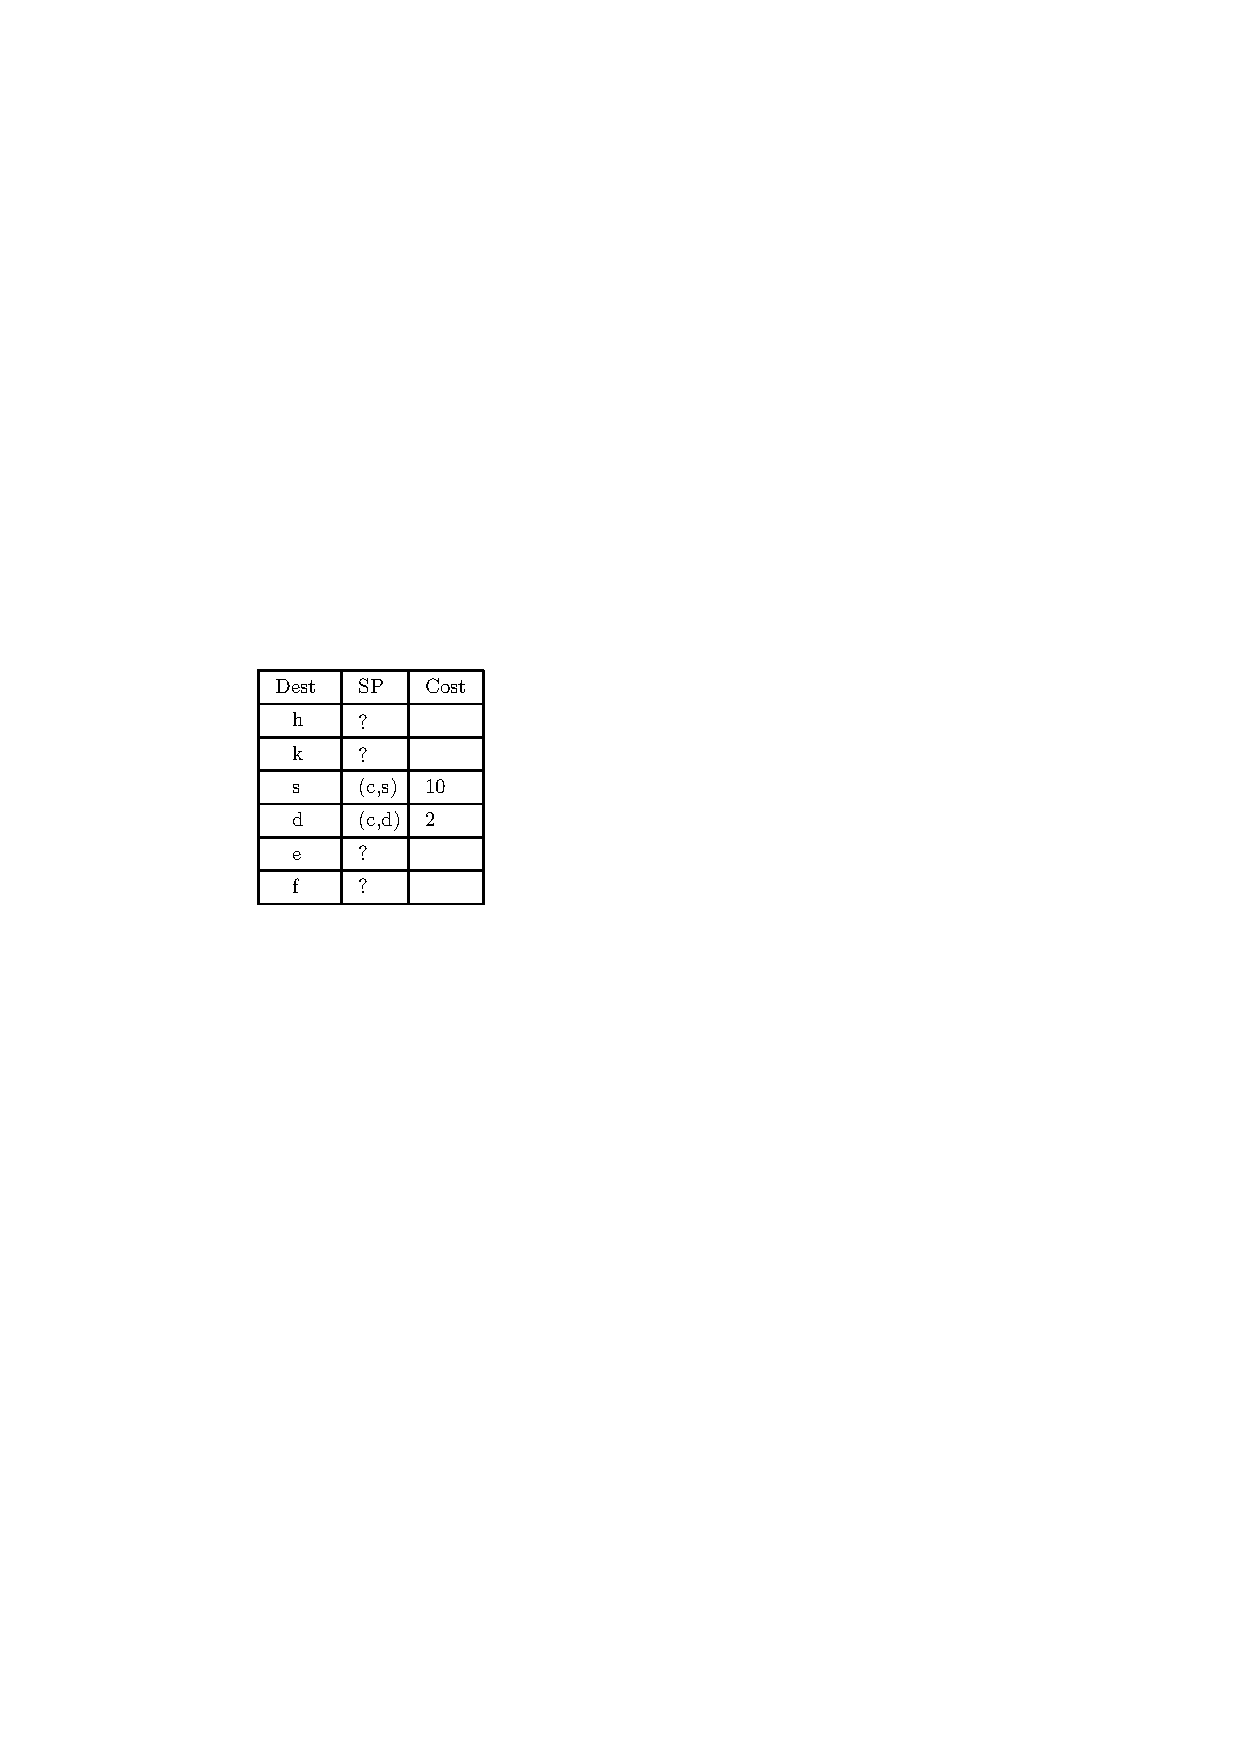
\includegraphics[scale=0.7]{routing_table_local_initial_c.pdf}
		\caption*{Tabella di $c$.}
	\end{figure}
\end{frame}

\begin{frame}
	\frametitle{}
	
	\begin{figure}[h]
	\centering
		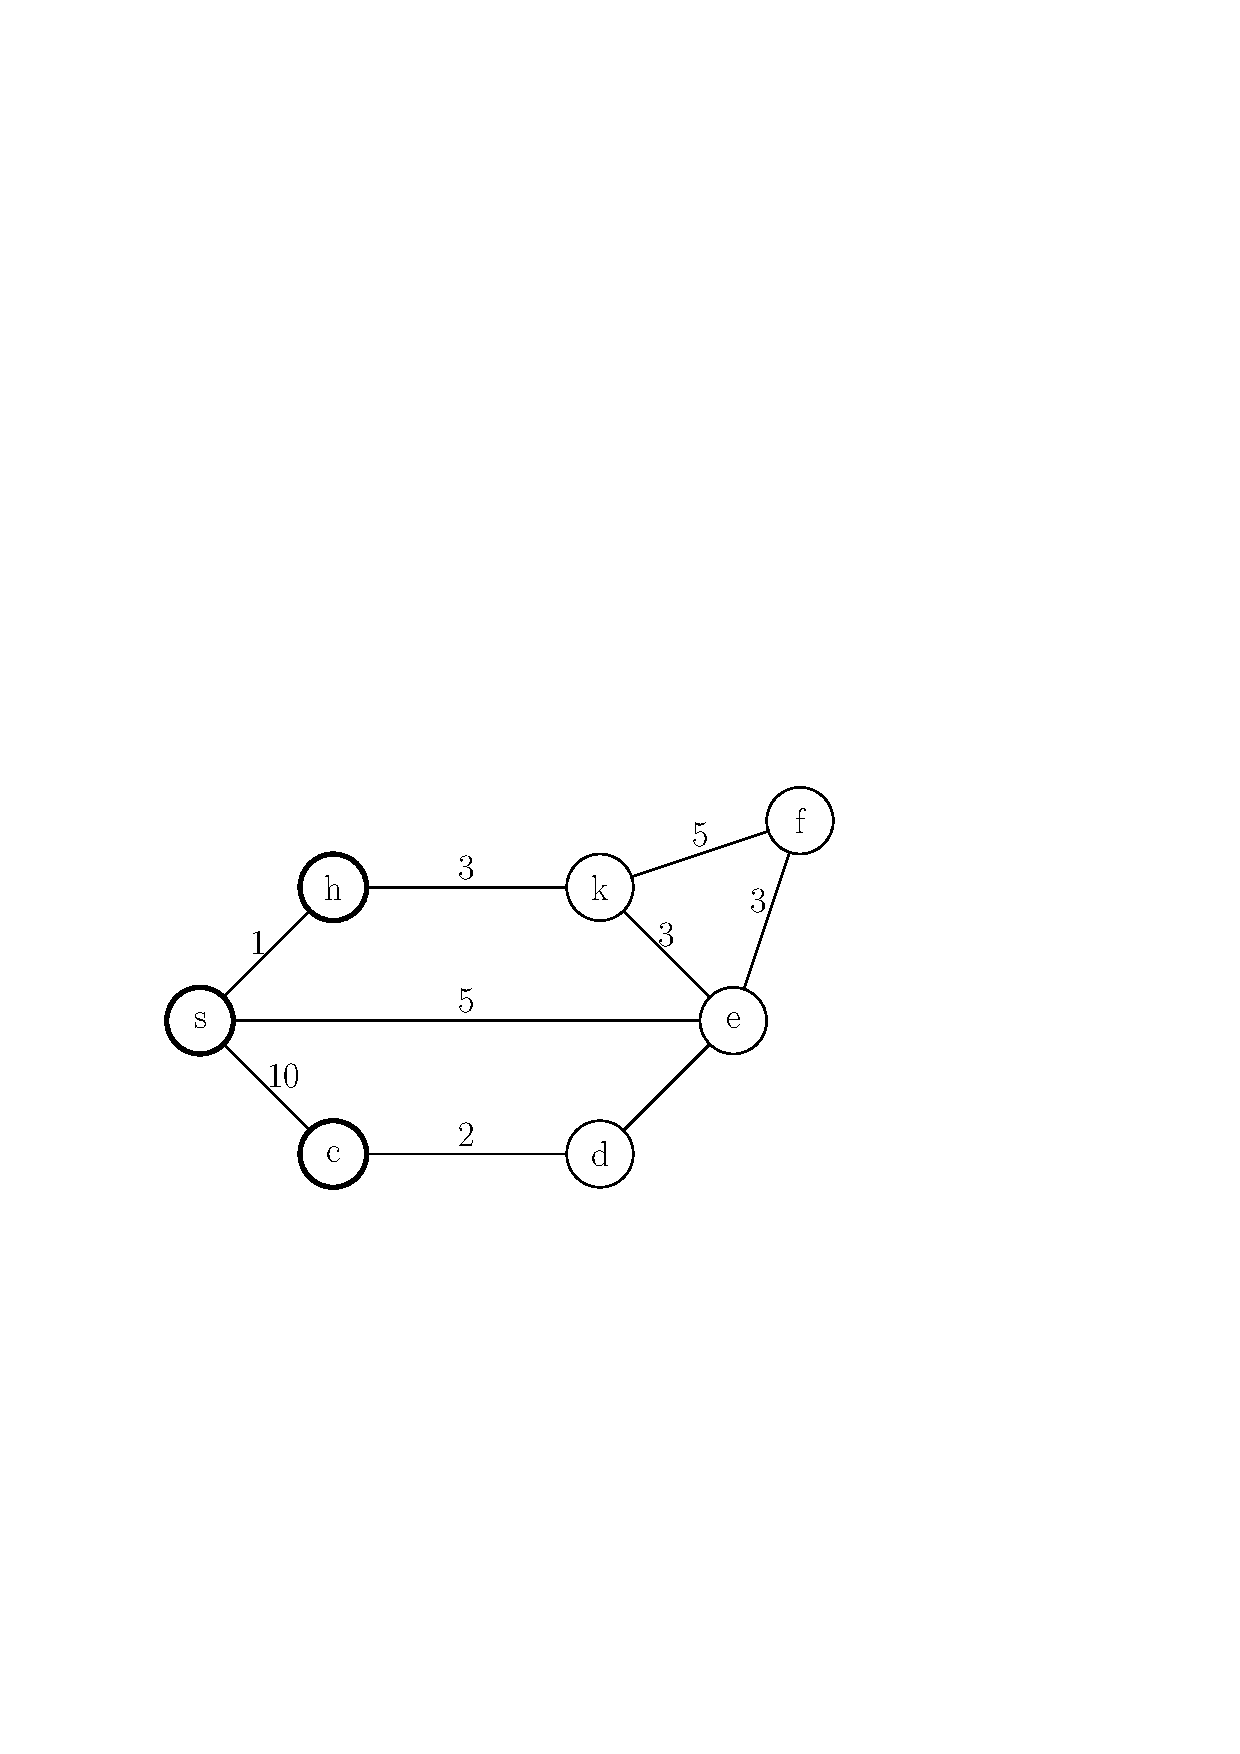
\includegraphics[scale=0.55]{routing_table_graph_receive.pdf}
	\end{figure}

	\begin{figure}[h]
	\centering
		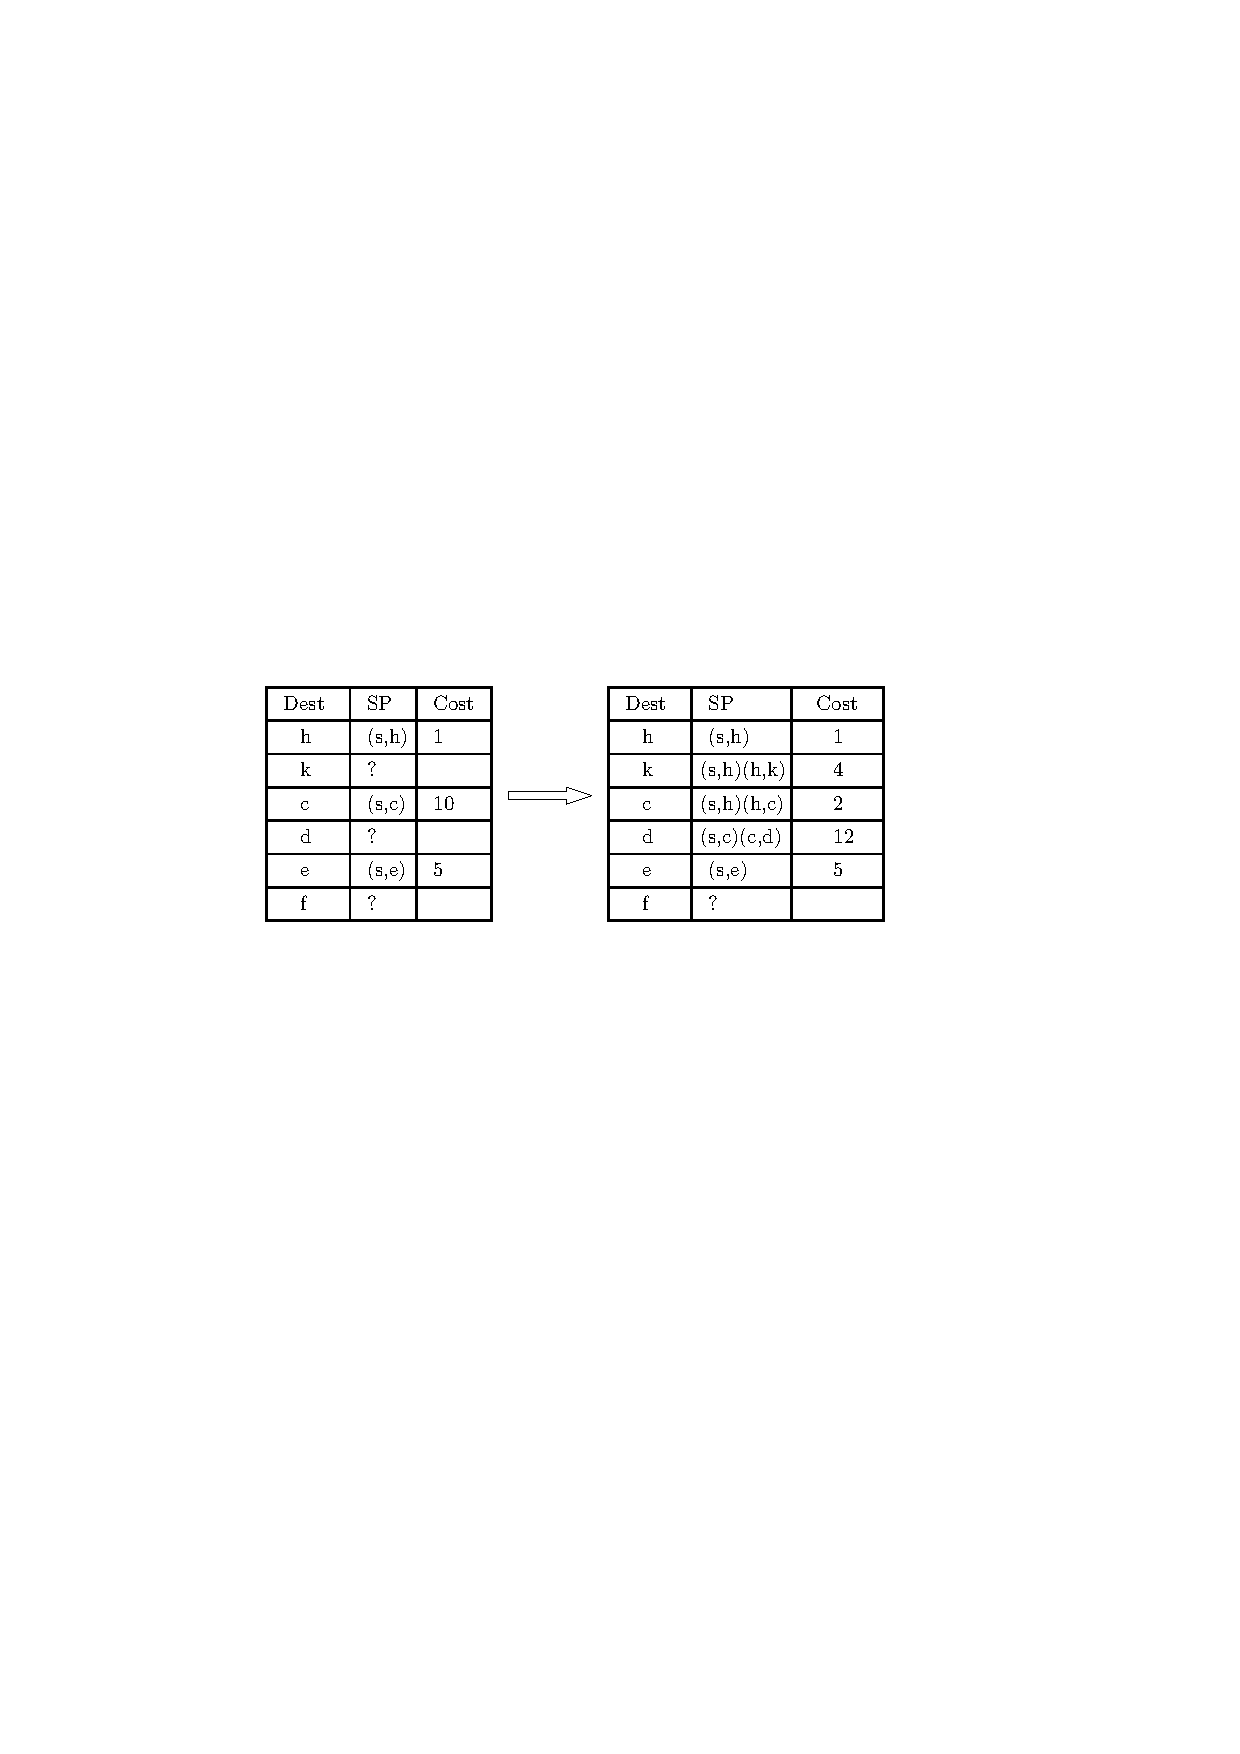
\includegraphics[width=.85\linewidth]{routing_table_local_update_s.pdf}
	\end{figure}
\end{frame}

\begin{frame}
	\frametitle{Message Complexity della Costruzione Iterativa}
	In al più $n-1$ iterazioni ogni nodo ha l'informazione corretta.
	\vfill

	\pause
	Ad ogni iterazione, ogni nodo $v$ invia $n$ items ai suoi $|N(v)|$ vicini.\\
	$\implies$ Messaggi per iterazione $= n \sum_v |N(v)|=2nm$.
	\vfill

	\pause
	Totale: $2(n-1)nm$
\end{frame}

\begin{frame}{}
	Per quanto abbiamo visto finora:
	\begin{itemize}
		\item \textbf{Map-Gossip}: usa tanta memoria.
		\item \textbf{Iterative-Construction}: meno memoria, ma più messaggi.
	\end{itemize}
	\vfill

	Possiamo trovare un compromesso?
\end{frame}

\begin{frame}
	\frametitle{}
	\textbf{Osservazione}: la tabella di routing globale di un nodo $v$ descrive uno spanning tree
	(l'albero dei cammini minimi di $v$).
	
	\begin{figure}[h]
	\centering
		\begin{subfigure}[b]{0.35\textwidth}
			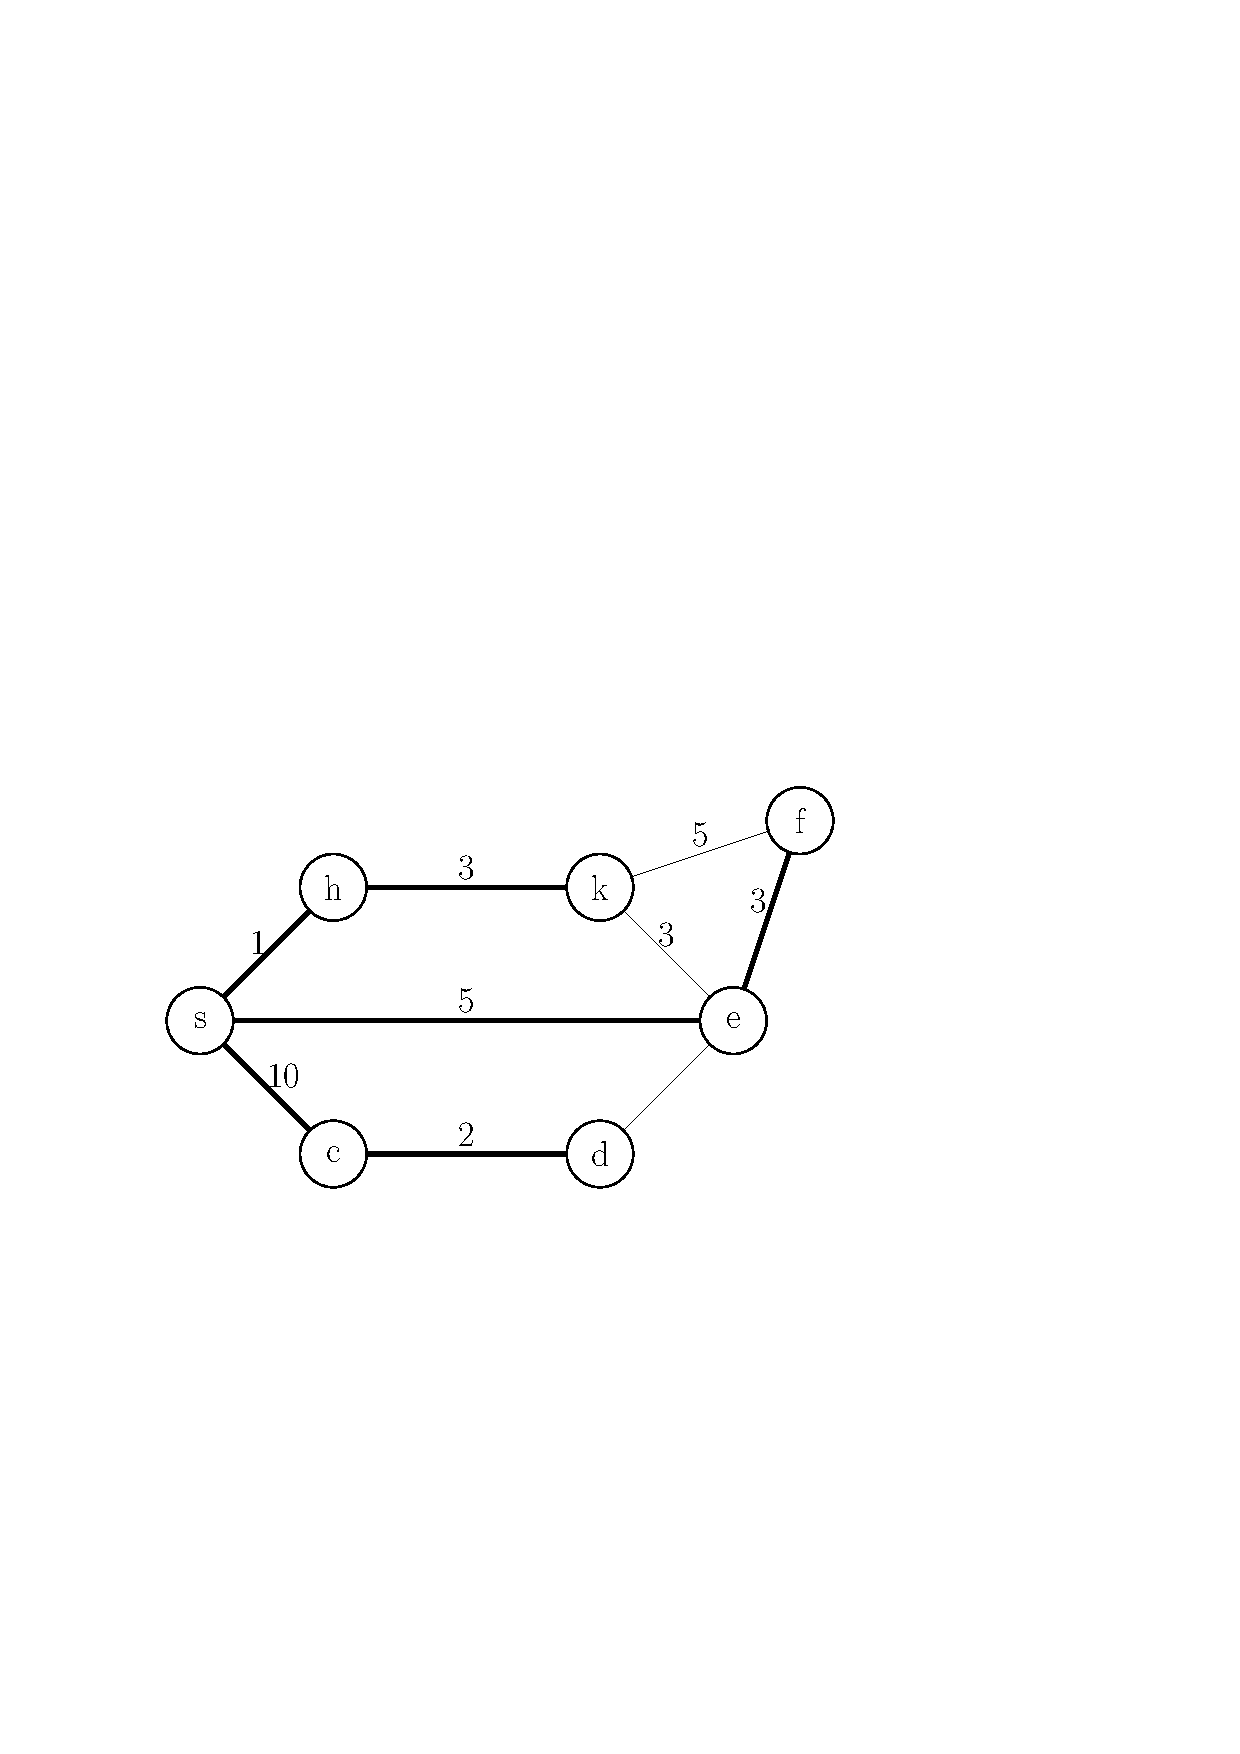
\includegraphics[scale=0.47]{routing_table_graph_tree.pdf}
		\end{subfigure}
		\begin{subfigure}[b]{0.6\textwidth}
			\hspace*{2cm}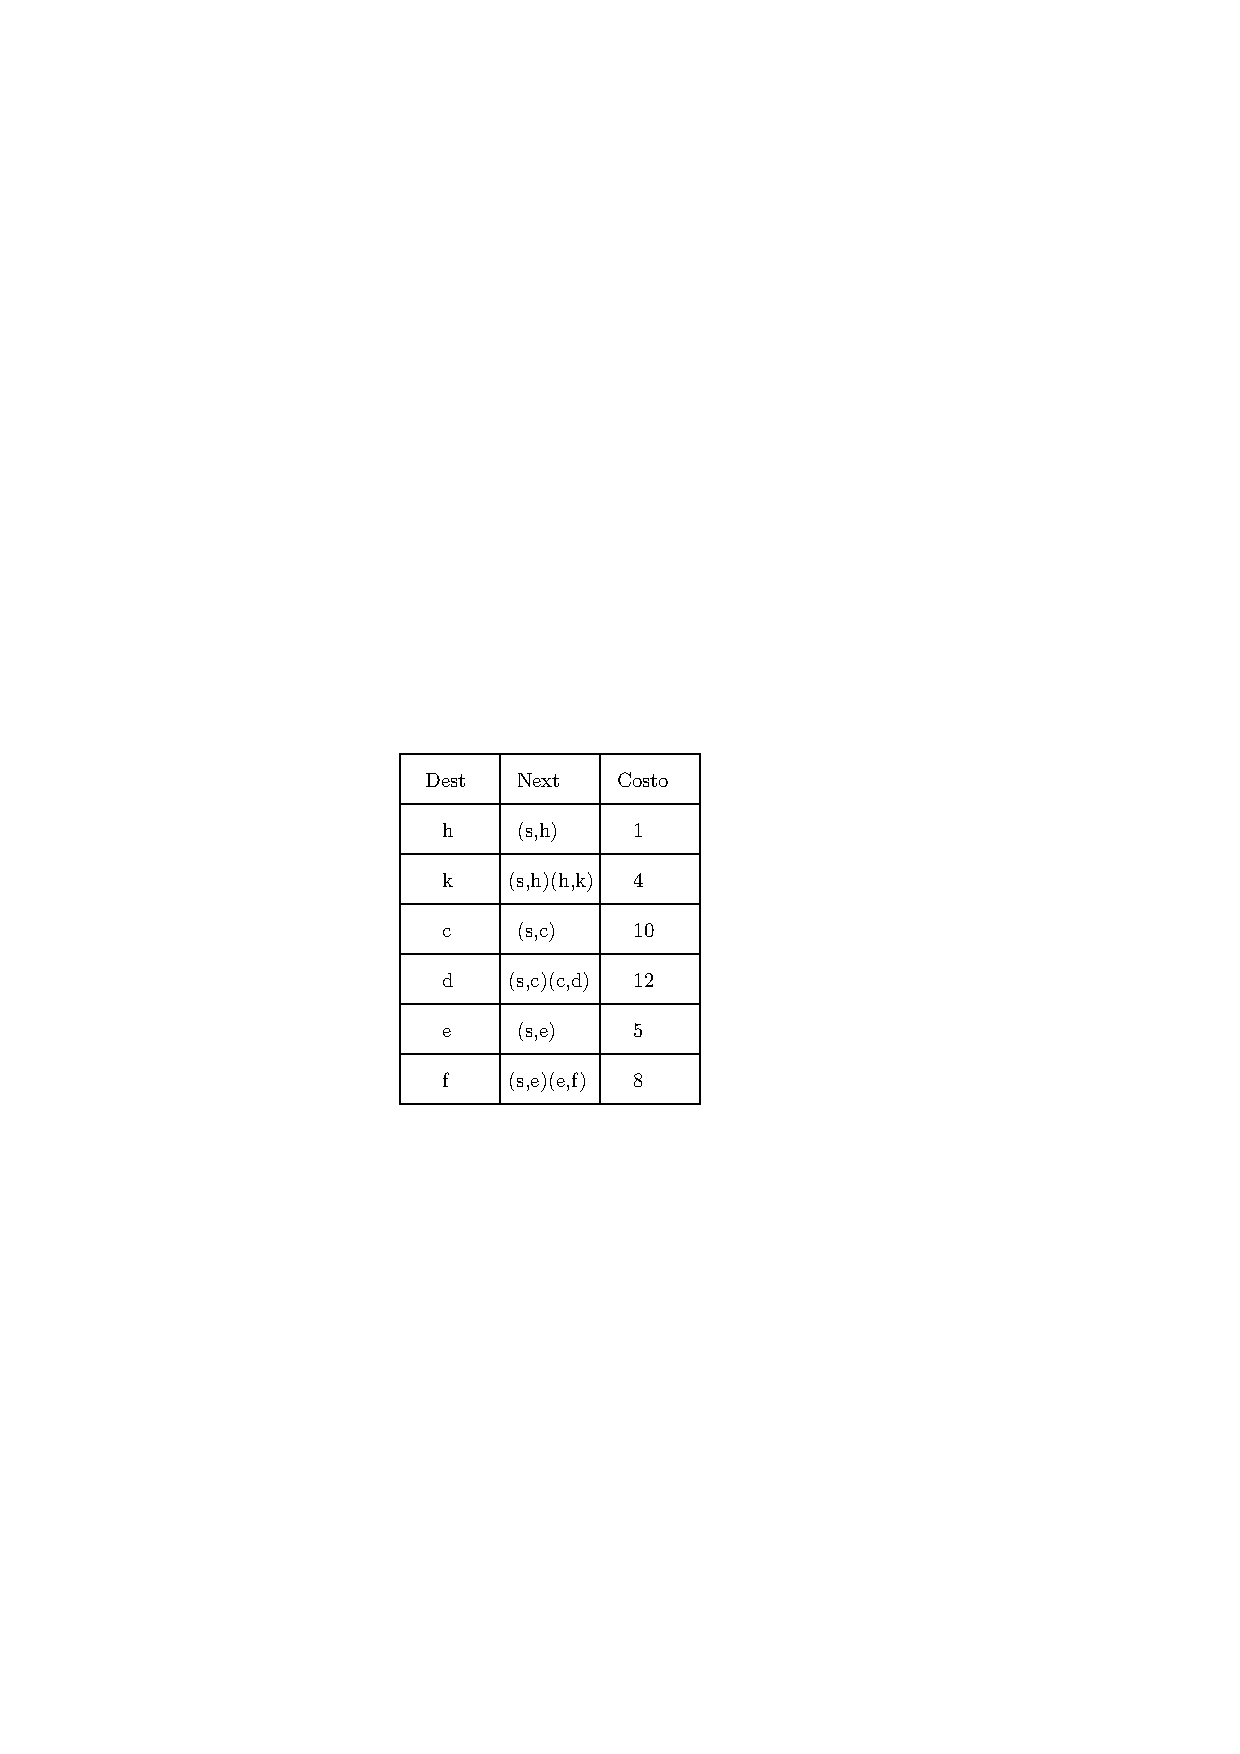
\includegraphics[scale=0.8]{routing_table_global.pdf}
		\end{subfigure}
	\end{figure}
\end{frame}

\begin{frame}
	\frametitle{Shortest Path Spanning Tree su Grafi Pesati}
	Per costruire la tabella di routing di $v$ è sufficiente costruire lo shortest path tree di $v$.
	\vfill

	\pause
	Algoritmo di Dijkstra (centralizzato, sequenziale) 
	\pause
	\\$\implies$ Versione Distribuita (PT-Construction)
\end{frame}

\begin{frame}
	\frametitle{L'algoritmo di Dijkstra}
	La distanza tra un nodo $u$ e un nodo $v$ è la lunghezza dello shortest path
	tra $u$ e $v$.
	\vfill

	L'algoritmo di Dijkstra calcola le distanze di tutti i vertici da un dato vertice iniziale $s$.
	\vfill

	\pause
	Assunzioni:
	\begin{itemize}
		\item il grafo è connesso,
		\item gli archi sono non-diretti,
		\item i pesi degli archi sono non-negativi.
	\end{itemize}
\end{frame}

\begin{frame}
	\frametitle{}
	\textbf{Greedy}: l'algoritmo fa crescere un sottoinsieme di nodi, 
	iniziando da $s$ e includendo infine tutti i nodi.
	\vfill

	In ogni nodo $v$ memorizziamo\\
	$d(v)=$ distanza di $v$ da $s$ nel sottografo che consiste dal sottinsieme attuale
	e dagli archi ad esso adiacenti.	
	
	\begin{figure}[h]
	\centering
		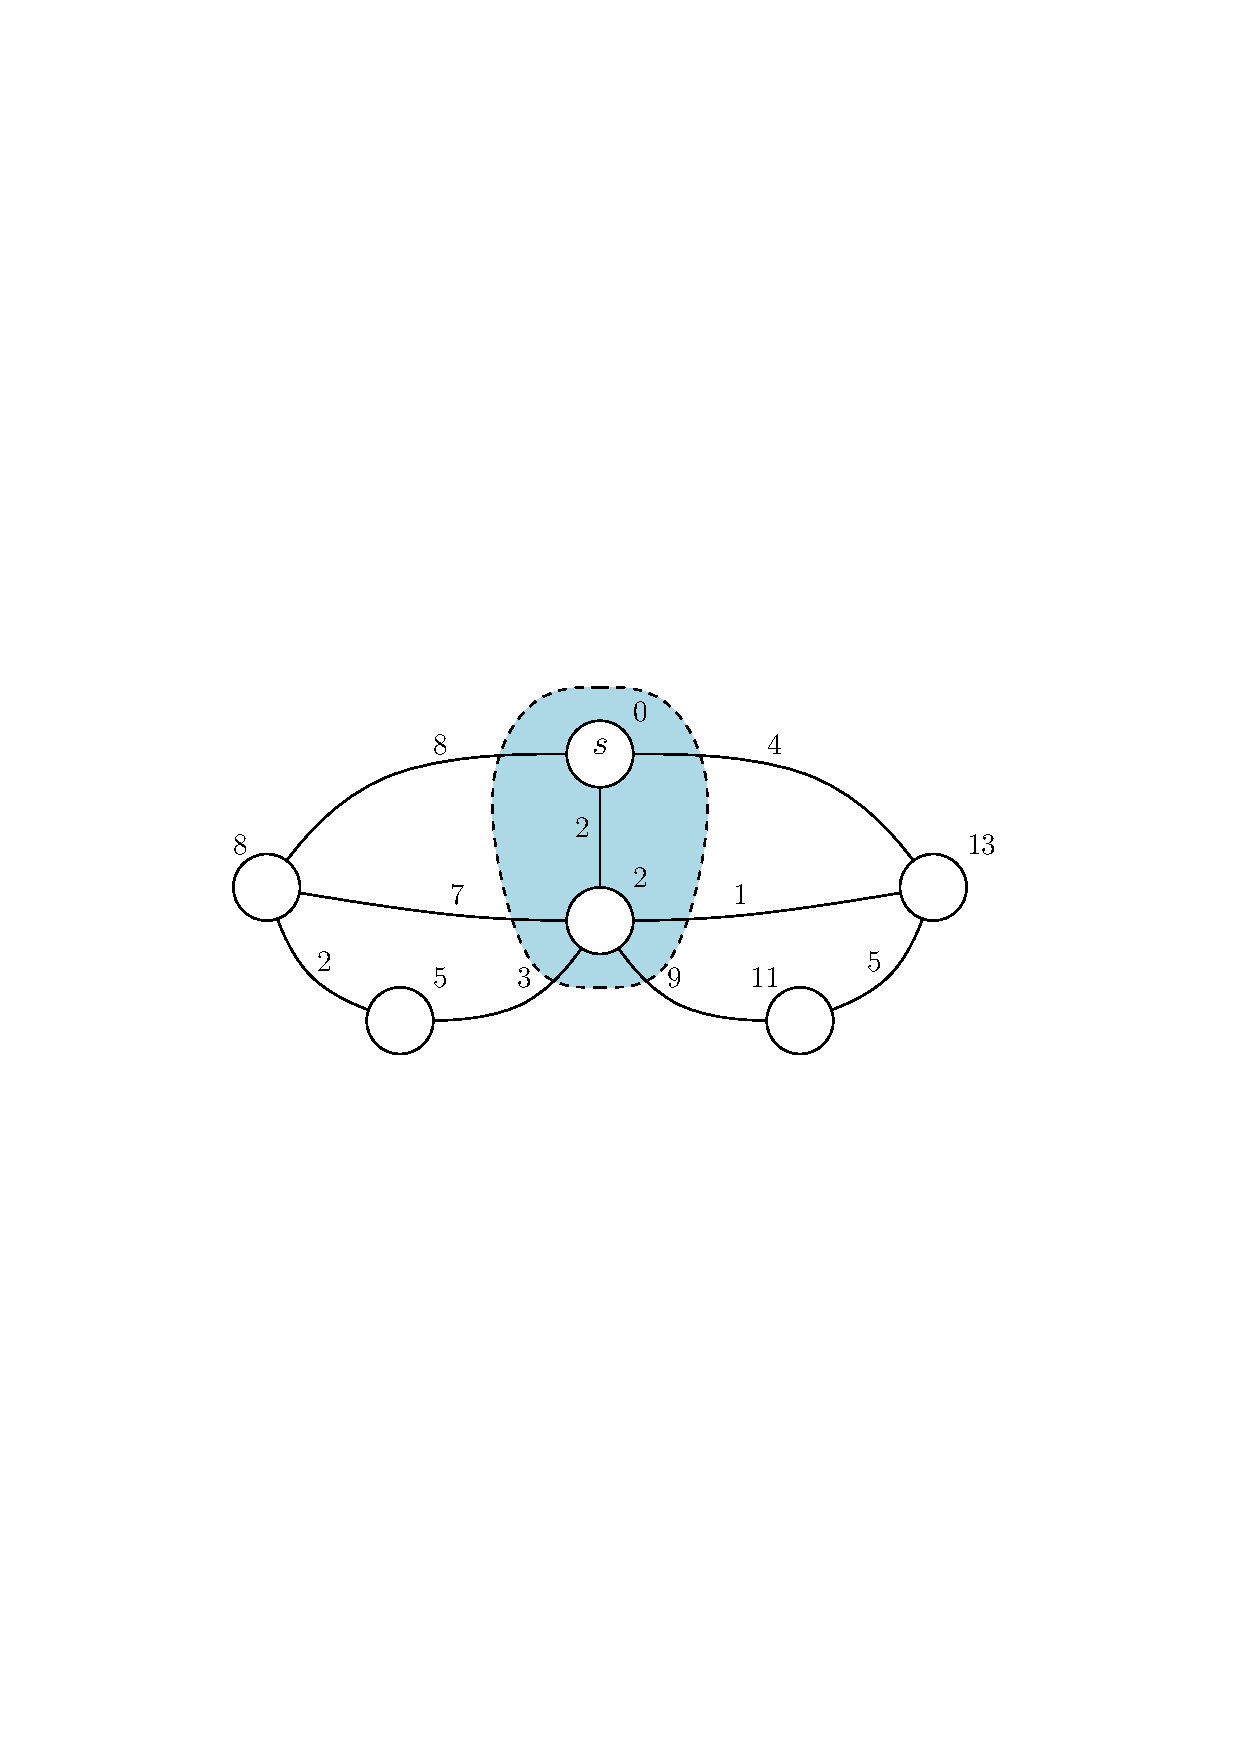
\includegraphics[scale=0.8]{dijkstra_example.pdf}
	\end{figure}
\end{frame}

\begin{frame}
	\frametitle{}
	Ad ogni passo
	\begin{itemize}
		\item Aggiungiamo all'insieme il nodo $u$ adiacente ad esso con la distanza più piccola
		\item Aggiorniamo le distanze dei vertici adiacenti ad $u$.
	\end{itemize}
	\vfill

	\begin{figure}[h]
	\centering
		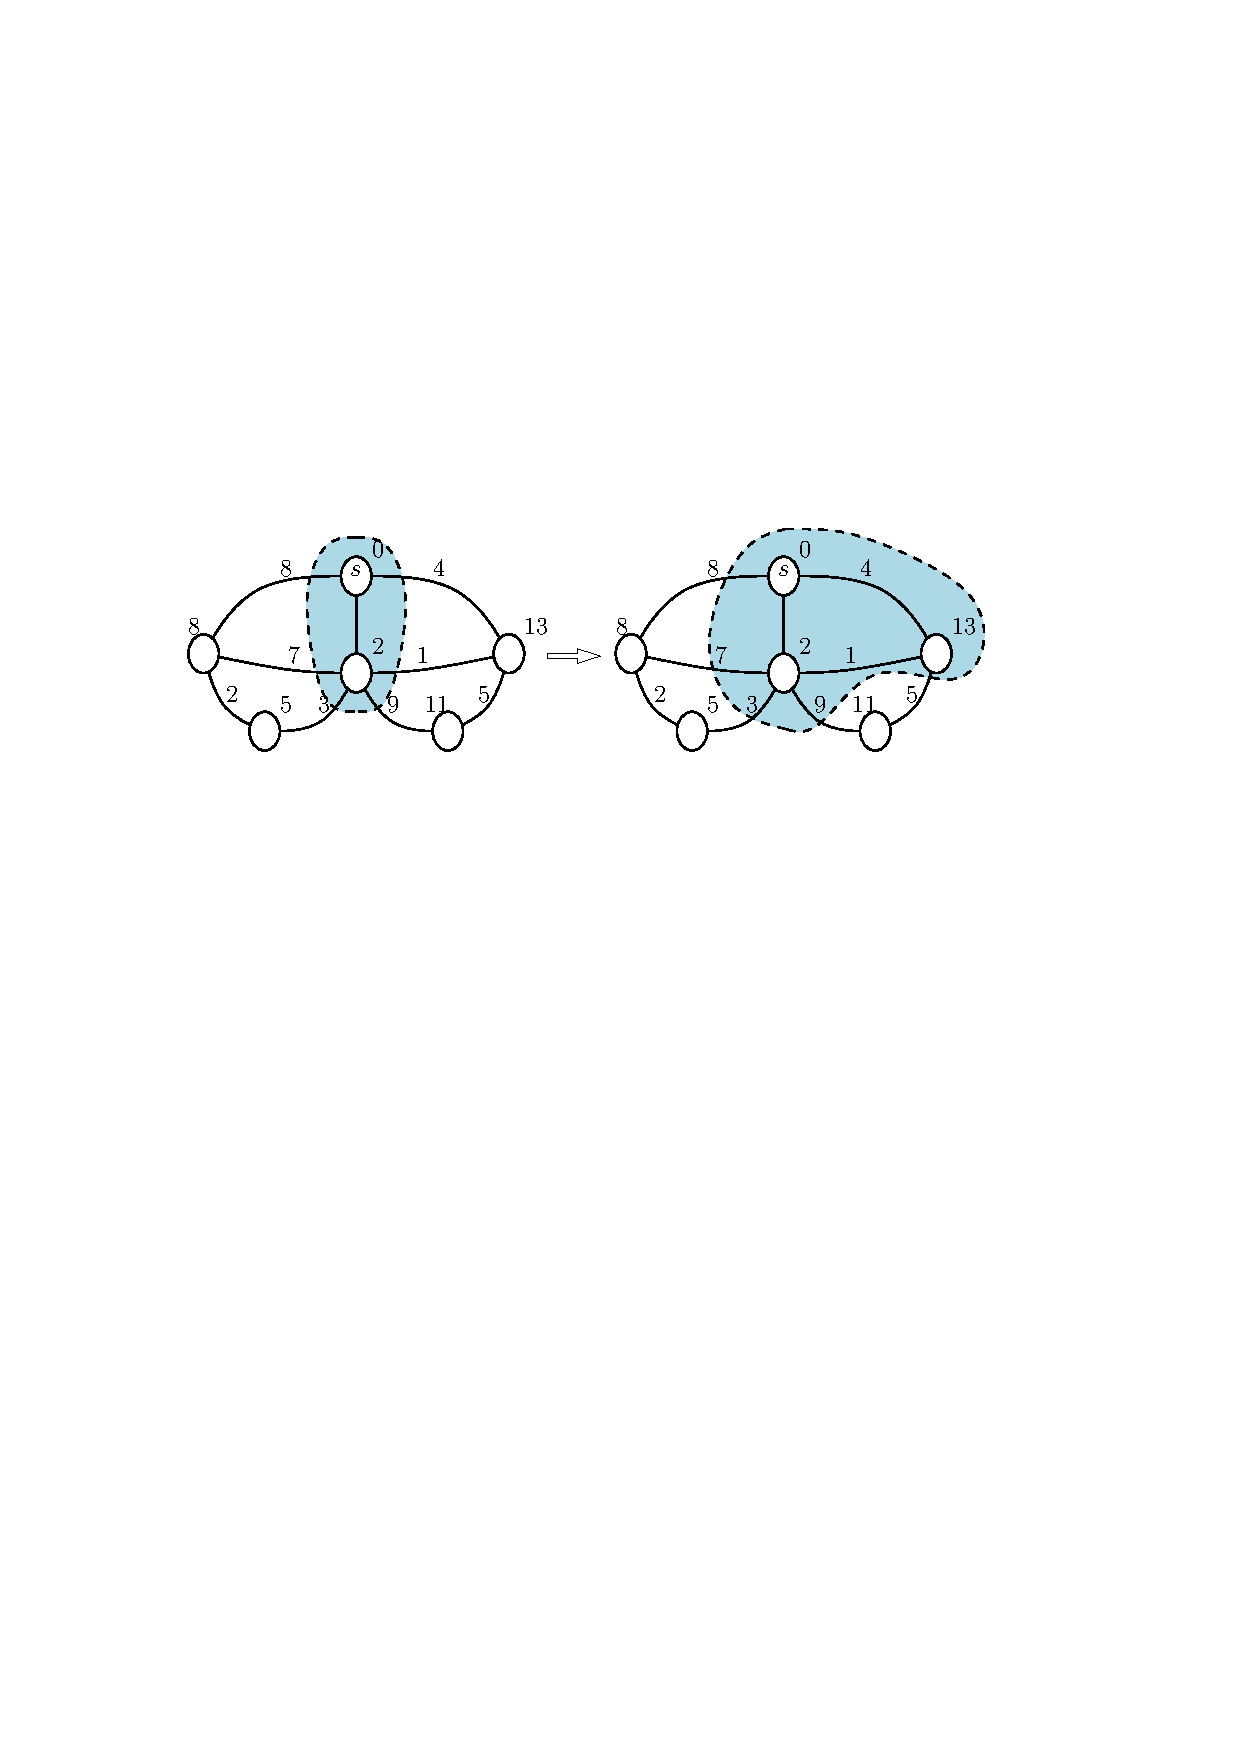
\includegraphics[scale=0.8]{dijkstra_update.pdf}
	\end{figure}
	\vfill
	
	Come eseguiamo l'update dei vicini di $u$?
\end{frame}

\begin{frame}
	\frametitle{Update = Rilassamento degli Archi}
	Consideriamo un arco $e=(u,v)$ tale che 
	\begin{itemize}
		\item $u$ è il vertice più recente aggiunto all'insieme,
		\item $v$ non è nell'insieme.
	\end{itemize}
	\vfill

	Il rilassamento dell'arco $e$ aggiorna la distanza $d(v)$ nel modo seguente
	$$ d(v)=\min\left\{ d(v),d(u)+w(e) \right\}$$
	\vfill

	\begin{figure}[h]
	\centering
		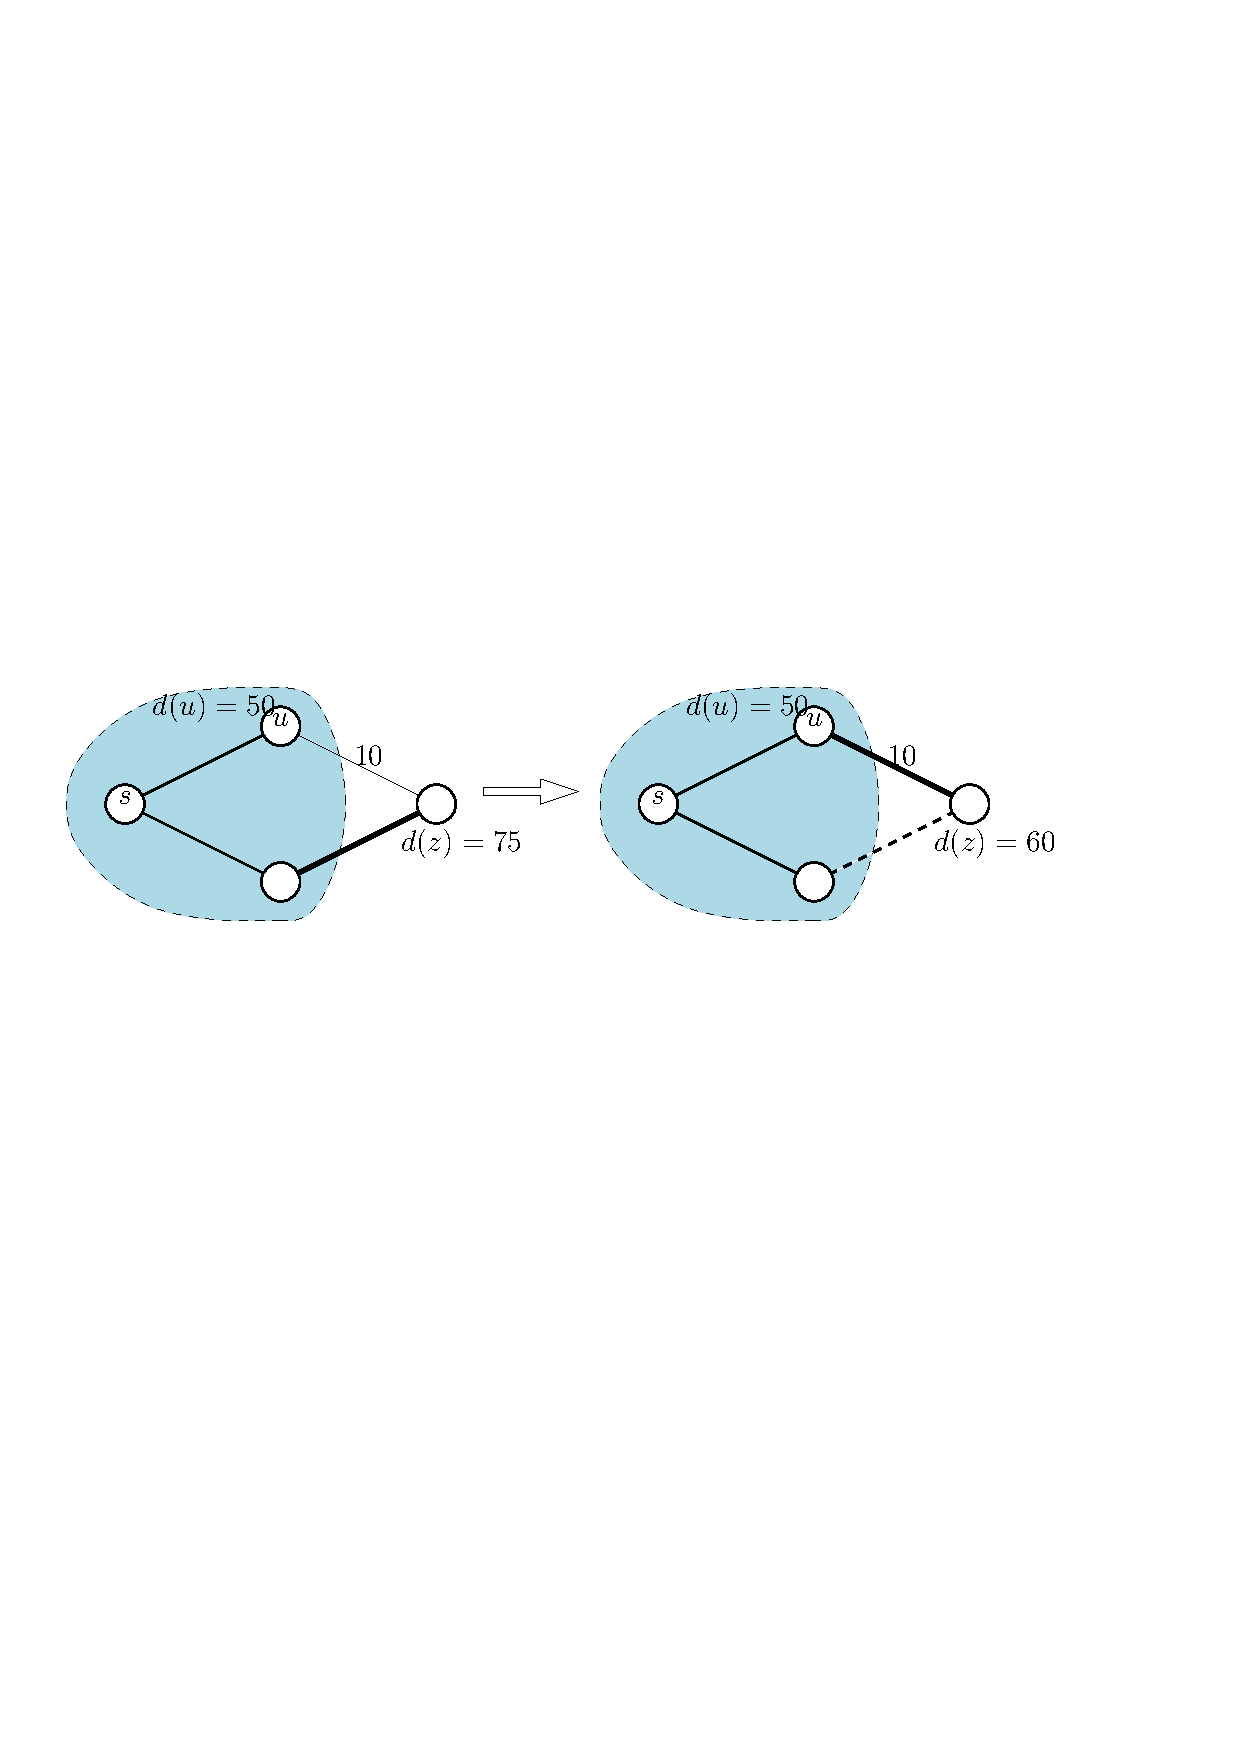
\includegraphics[scale=0.6]{dijkstra_relax.pdf}
	\end{figure}
\end{frame}

\begin{frame}
	\frametitle{}
	
	\begin{figure}[h]
	\centering
		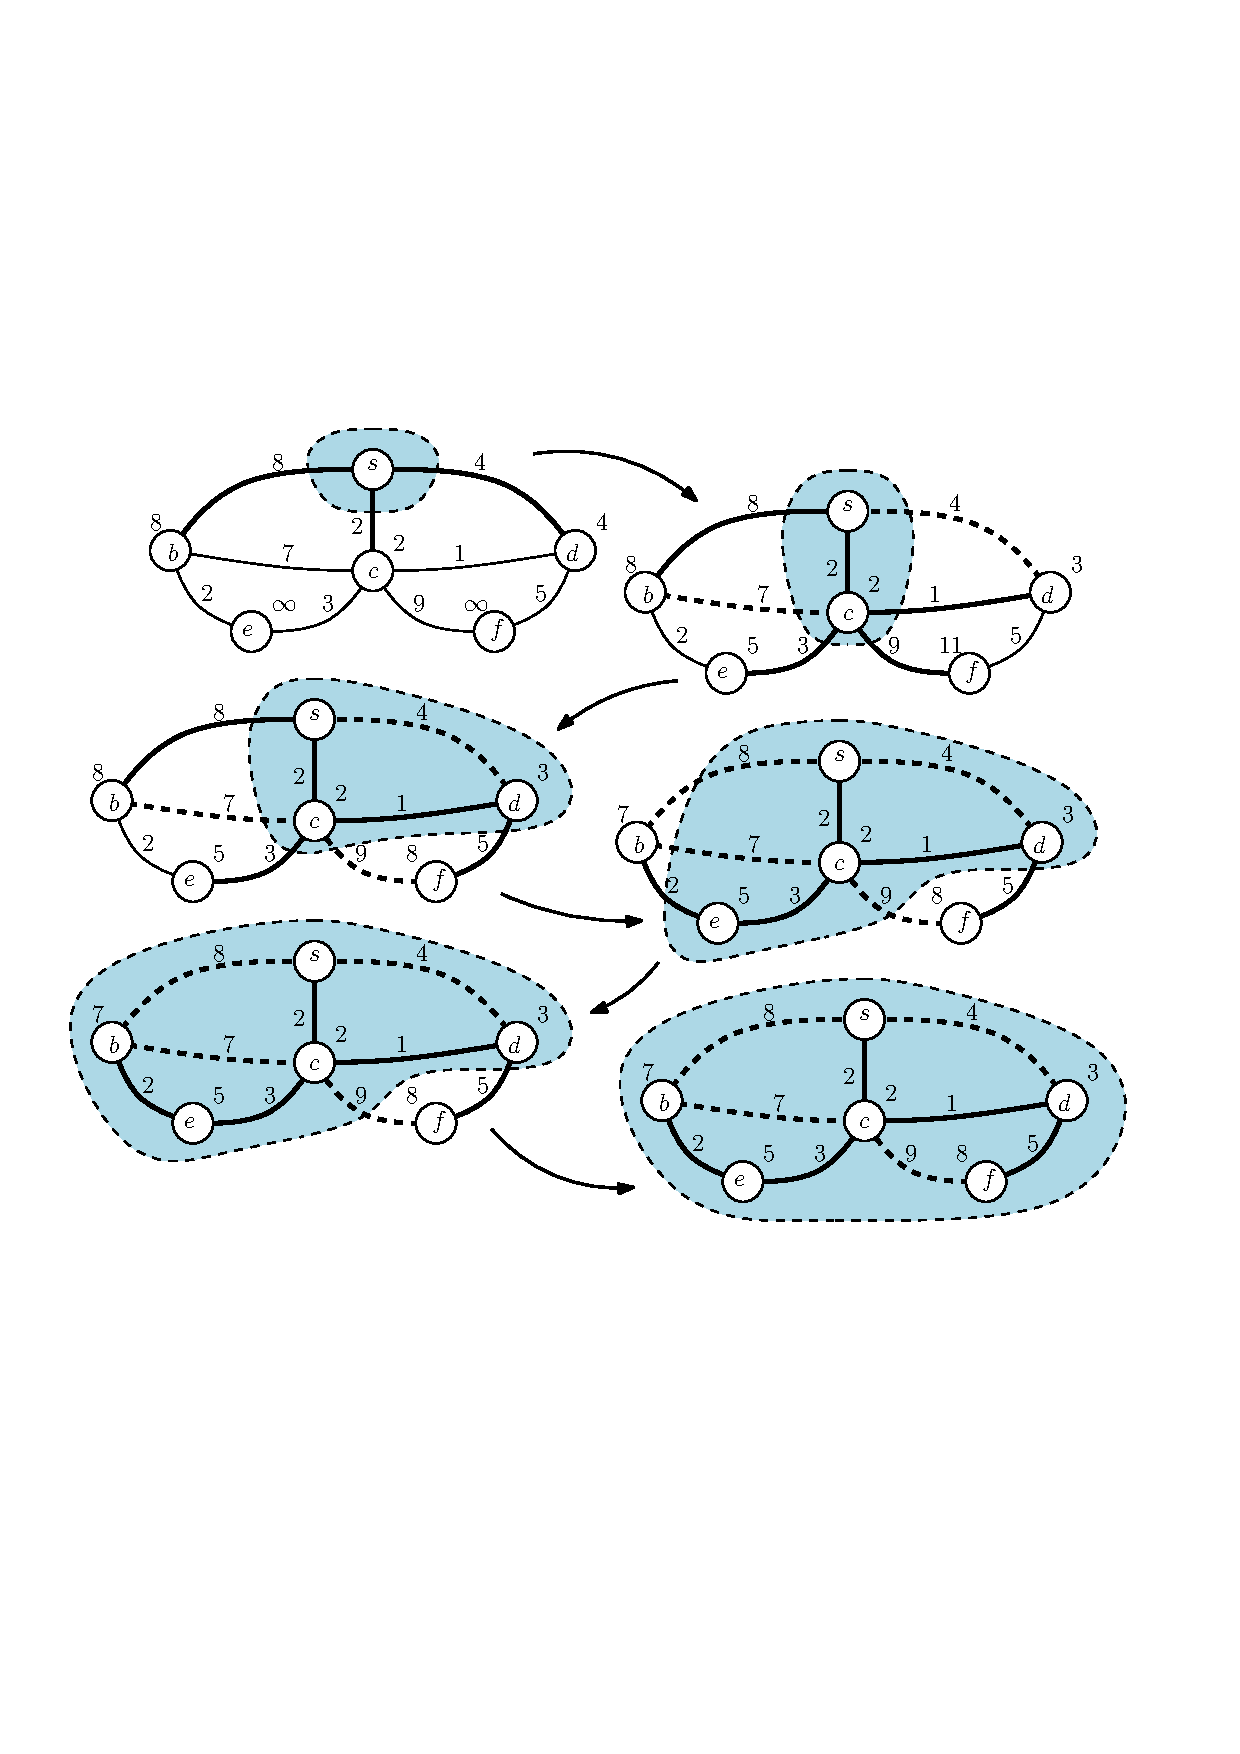
\includegraphics[scale=0.6]{dijkstra_process.pdf}
	\end{figure}
\end{frame}

\begin{frame}
	\frametitle{Versione distribuita: PT-Construction}
	La radice diffonde in $T$ l'inizio di una nuova iterazione.
	\begin{figure}[h]
	\centering
		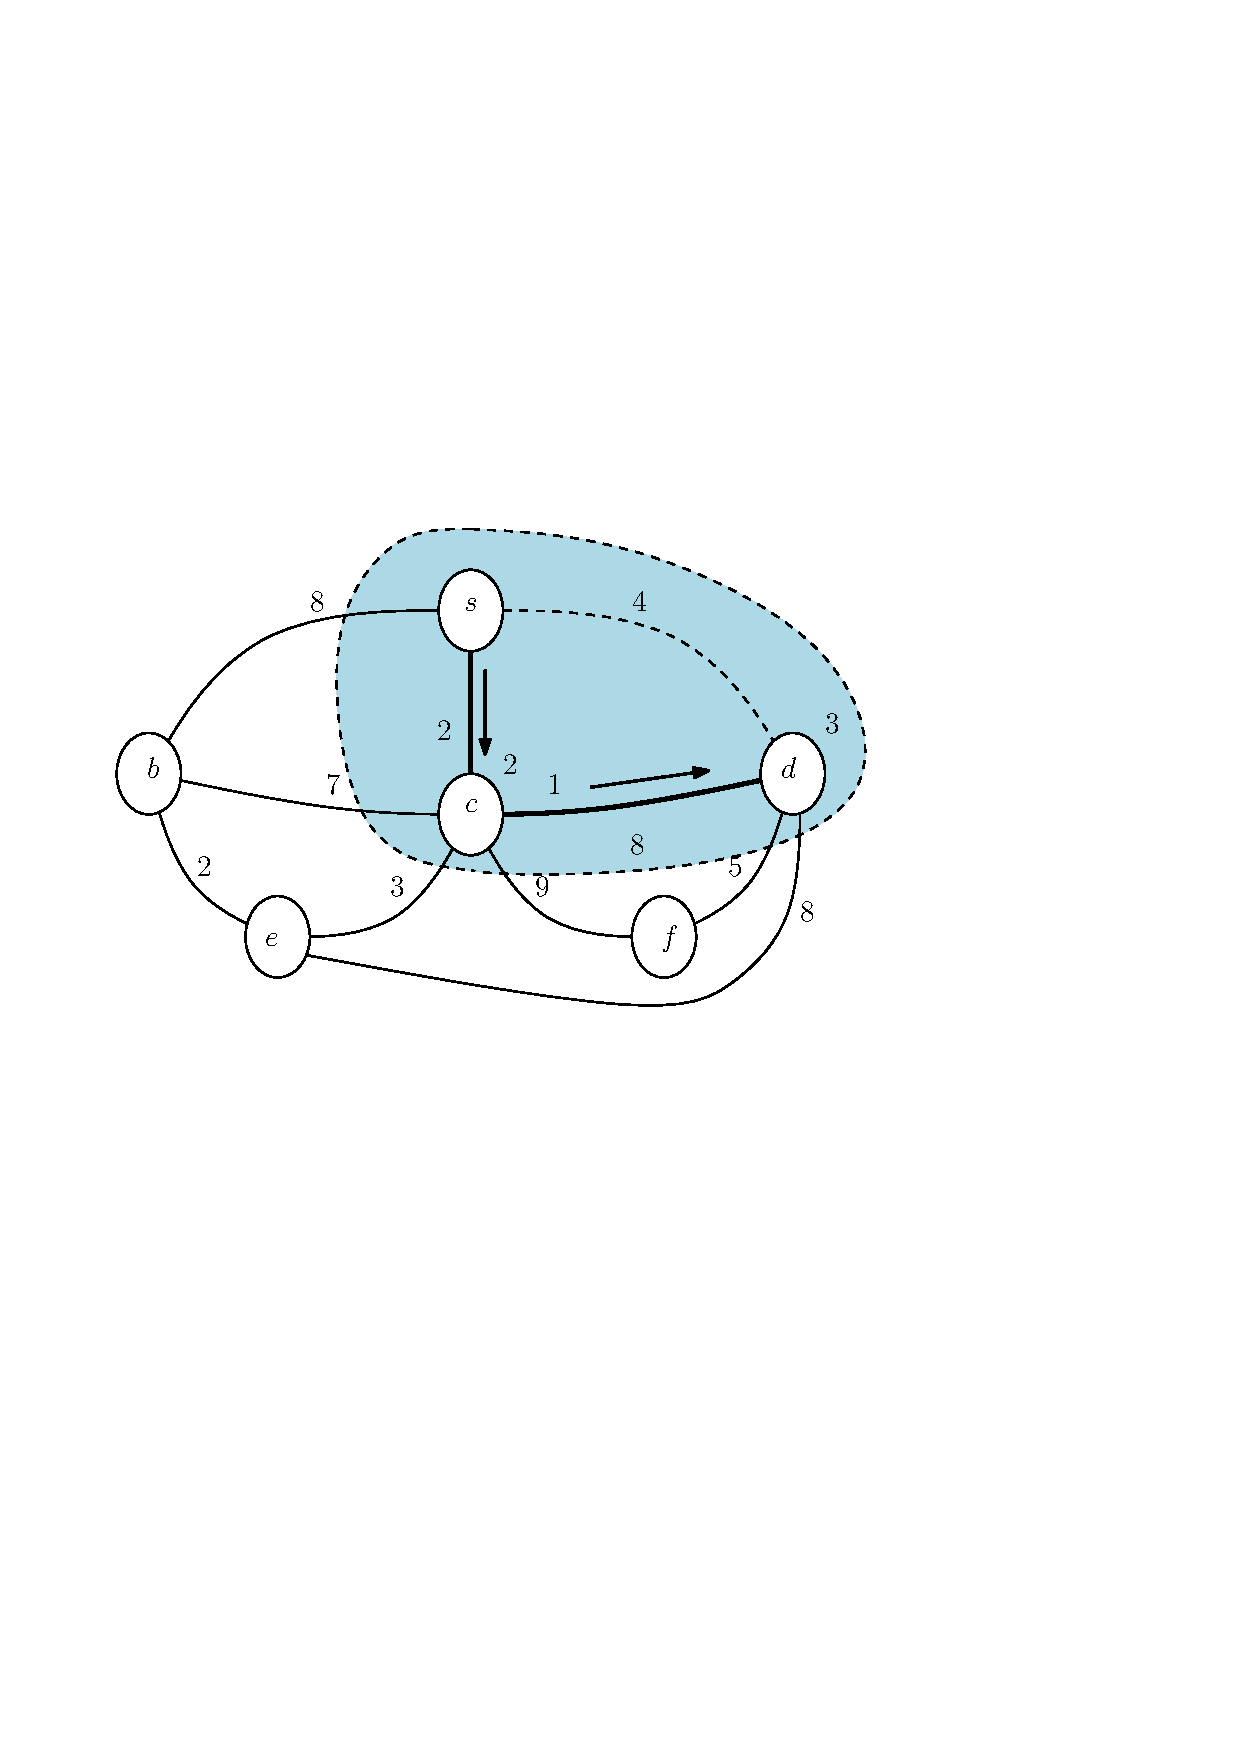
\includegraphics[scale=0.6]{PT1.pdf}
	\end{figure}
\end{frame}

\begin{frame}
	Ogni nodo in $T$ calcola localmente la distanza più breve 
		\textit{dalla radice ai vicini di T}.
	\begin{figure}[h]
	\centering
		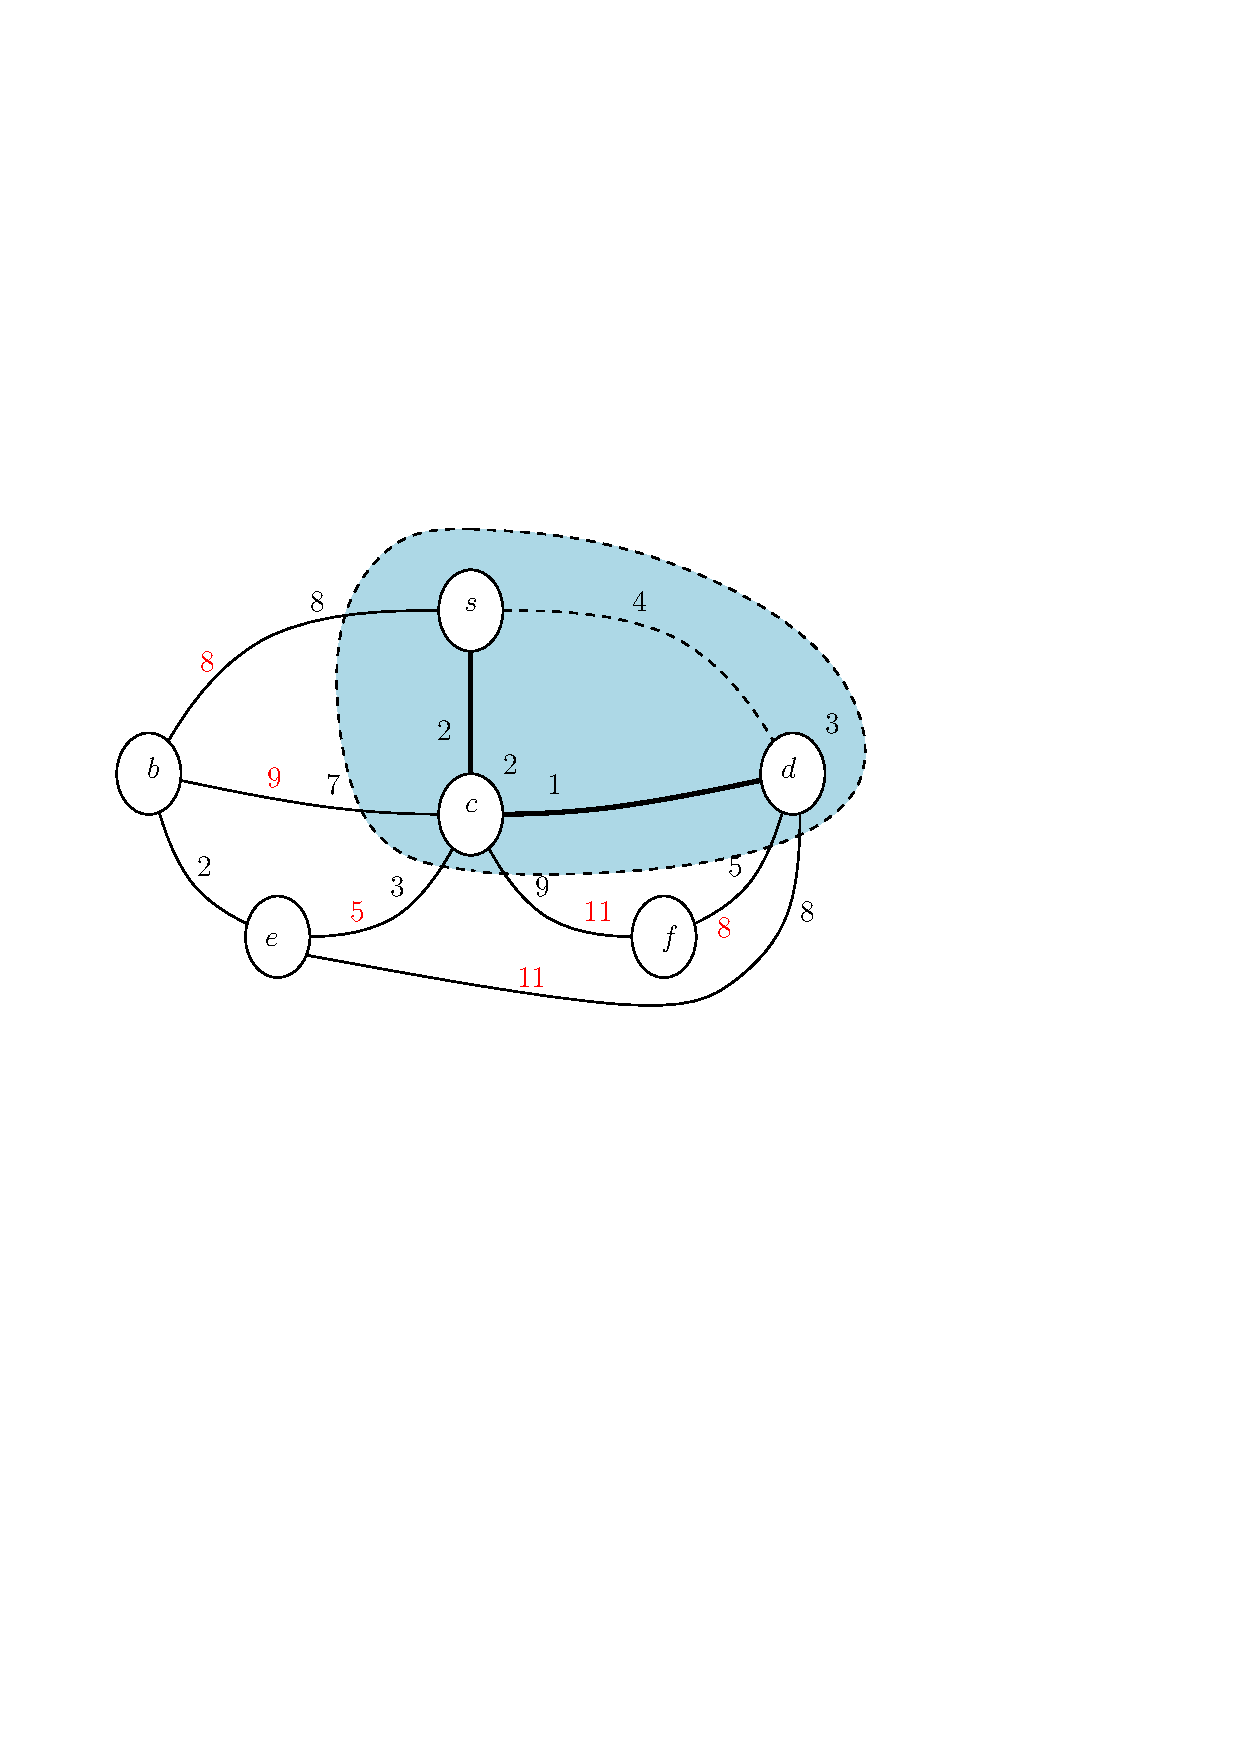
\includegraphics[scale=0.6]{PT2.pdf}
	\end{figure}
\end{frame}

\begin{frame}
	\frametitle{}
	Il minimo globale è calcolato alla radice, e il link corrispondente
	è scelto.
	\begin{figure}[h]
	\centering
		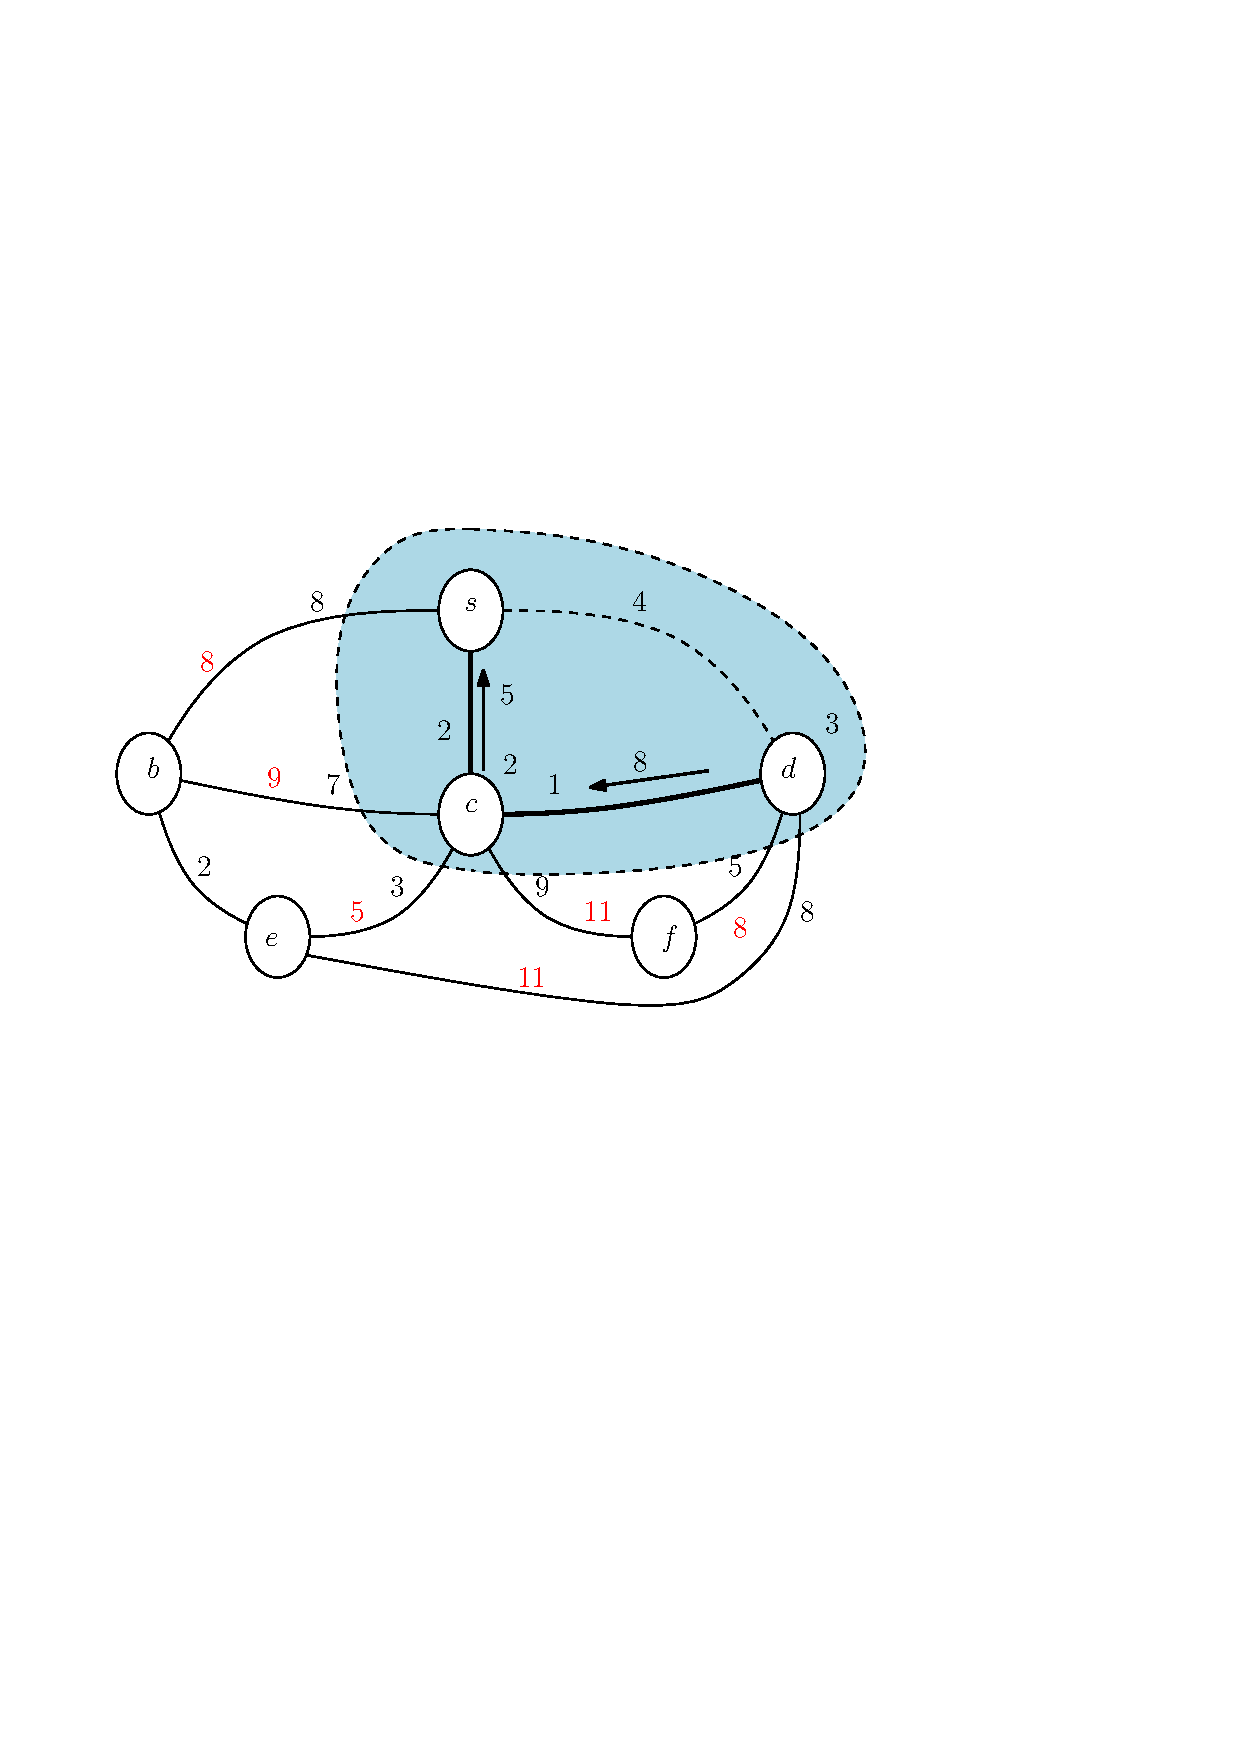
\includegraphics[scale=0.6]{PT3.pdf}
	\end{figure}
\end{frame}

\begin{frame}
	\frametitle{}
	La radice notifica il corrispondente nodo della scelta.
	\begin{figure}[h]
	\centering
		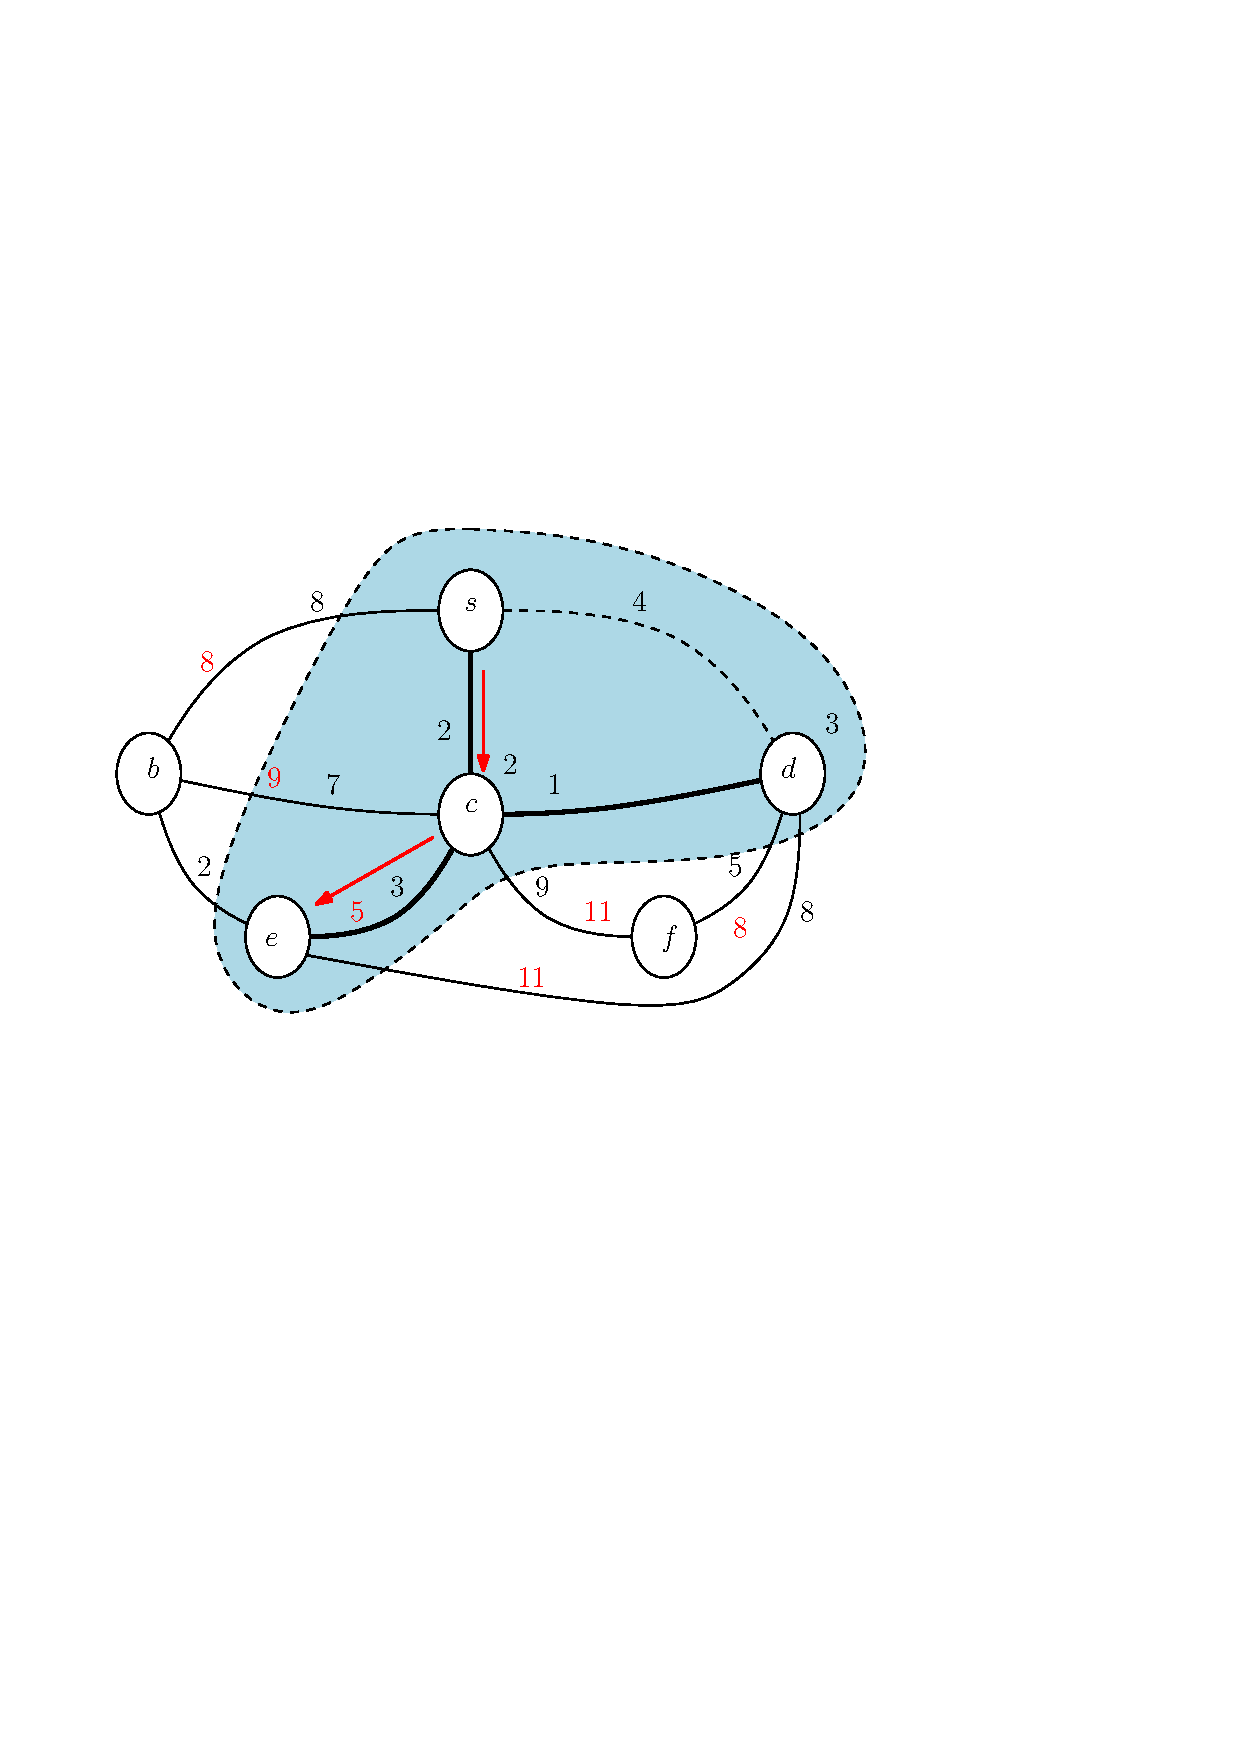
\includegraphics[scale=0.6]{PT4.pdf}
	\end{figure}
\end{frame}

\begin{frame}
	\frametitle{}
		Il nodo notificato informa i suoi vicini in modo che si possano formare
		i nuovi link interni.
	\begin{figure}[h]
	\centering
		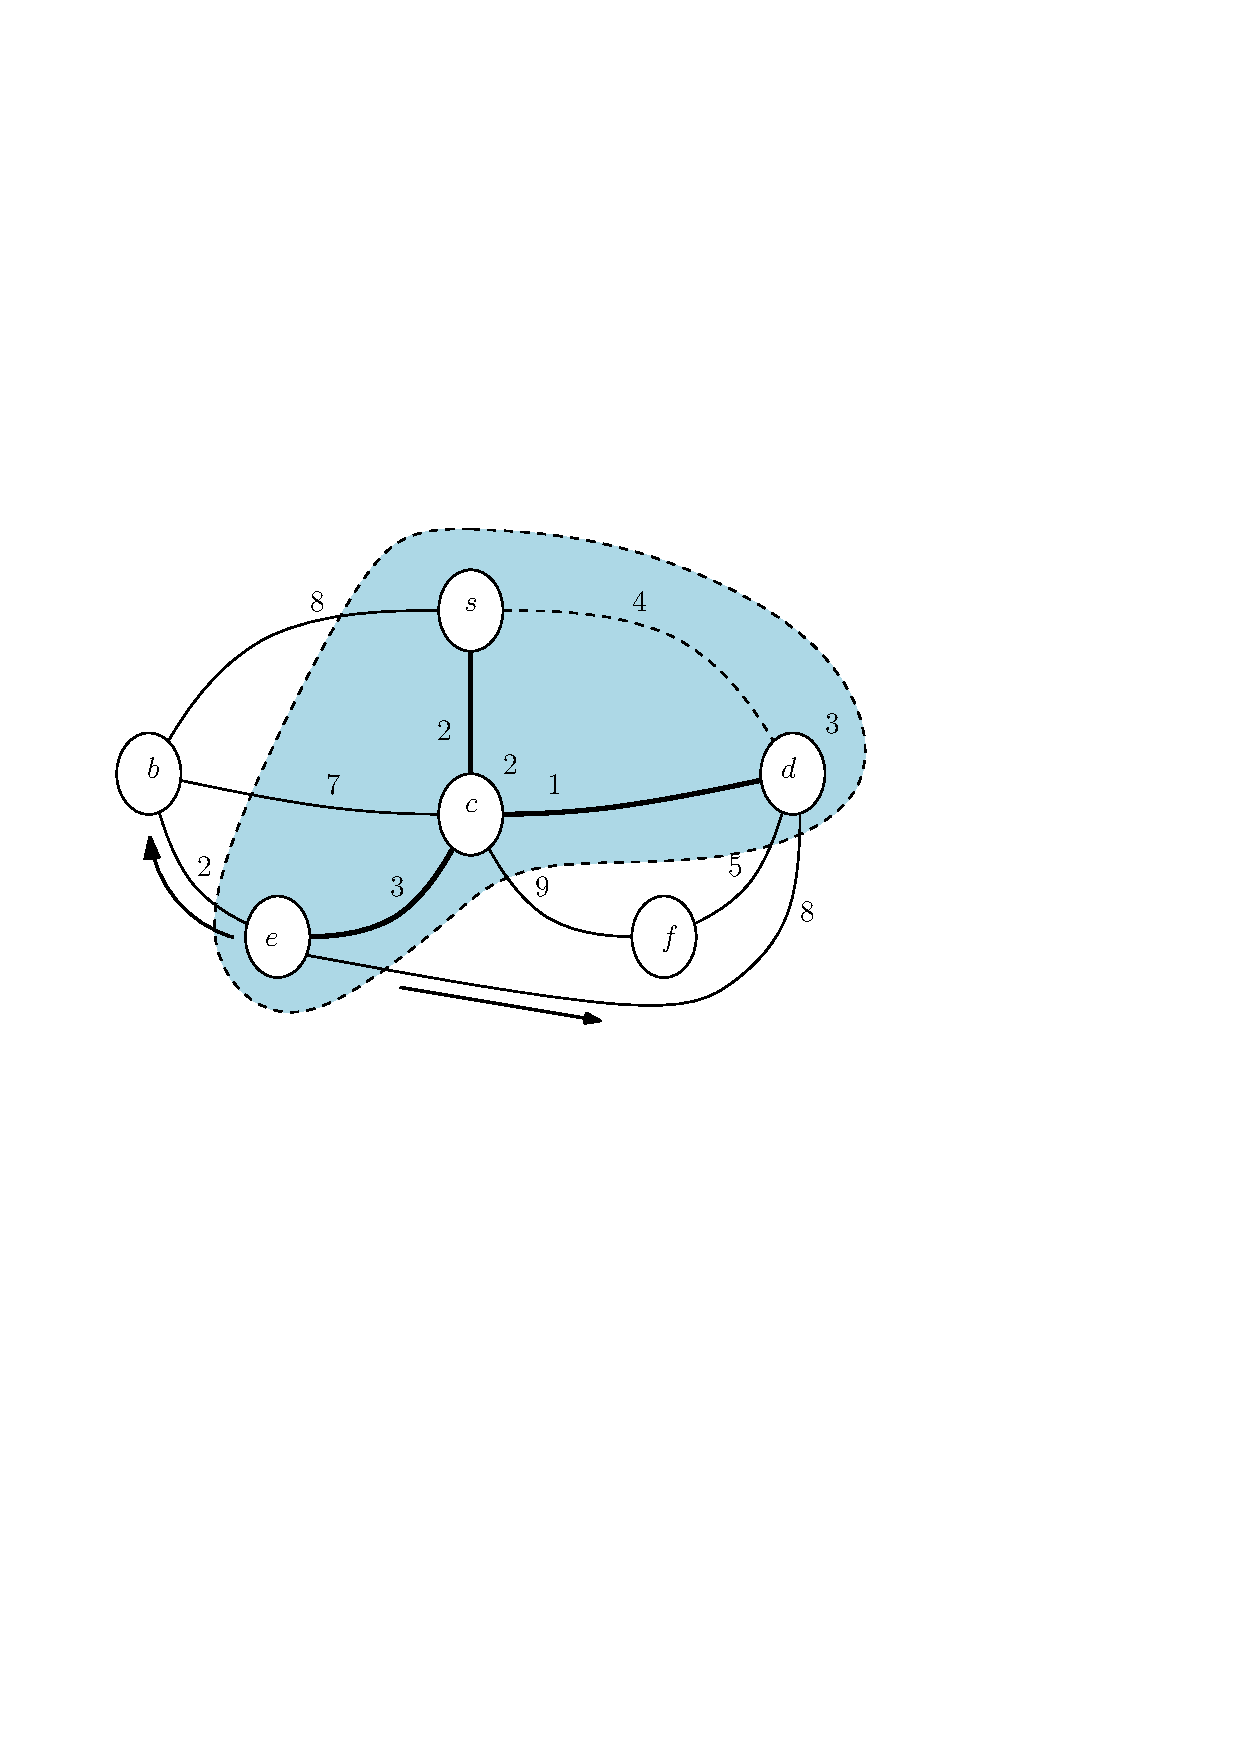
\includegraphics[scale=0.6]{PT5.pdf}
	\end{figure}
\end{frame}

\begin{frame}
	\frametitle{}
	Dopo aver ricevuto gli acknoledgement, il nodo notificato
	informa la radice della terminazione dell'iterazione. 
	\begin{figure}[h]
	\centering
		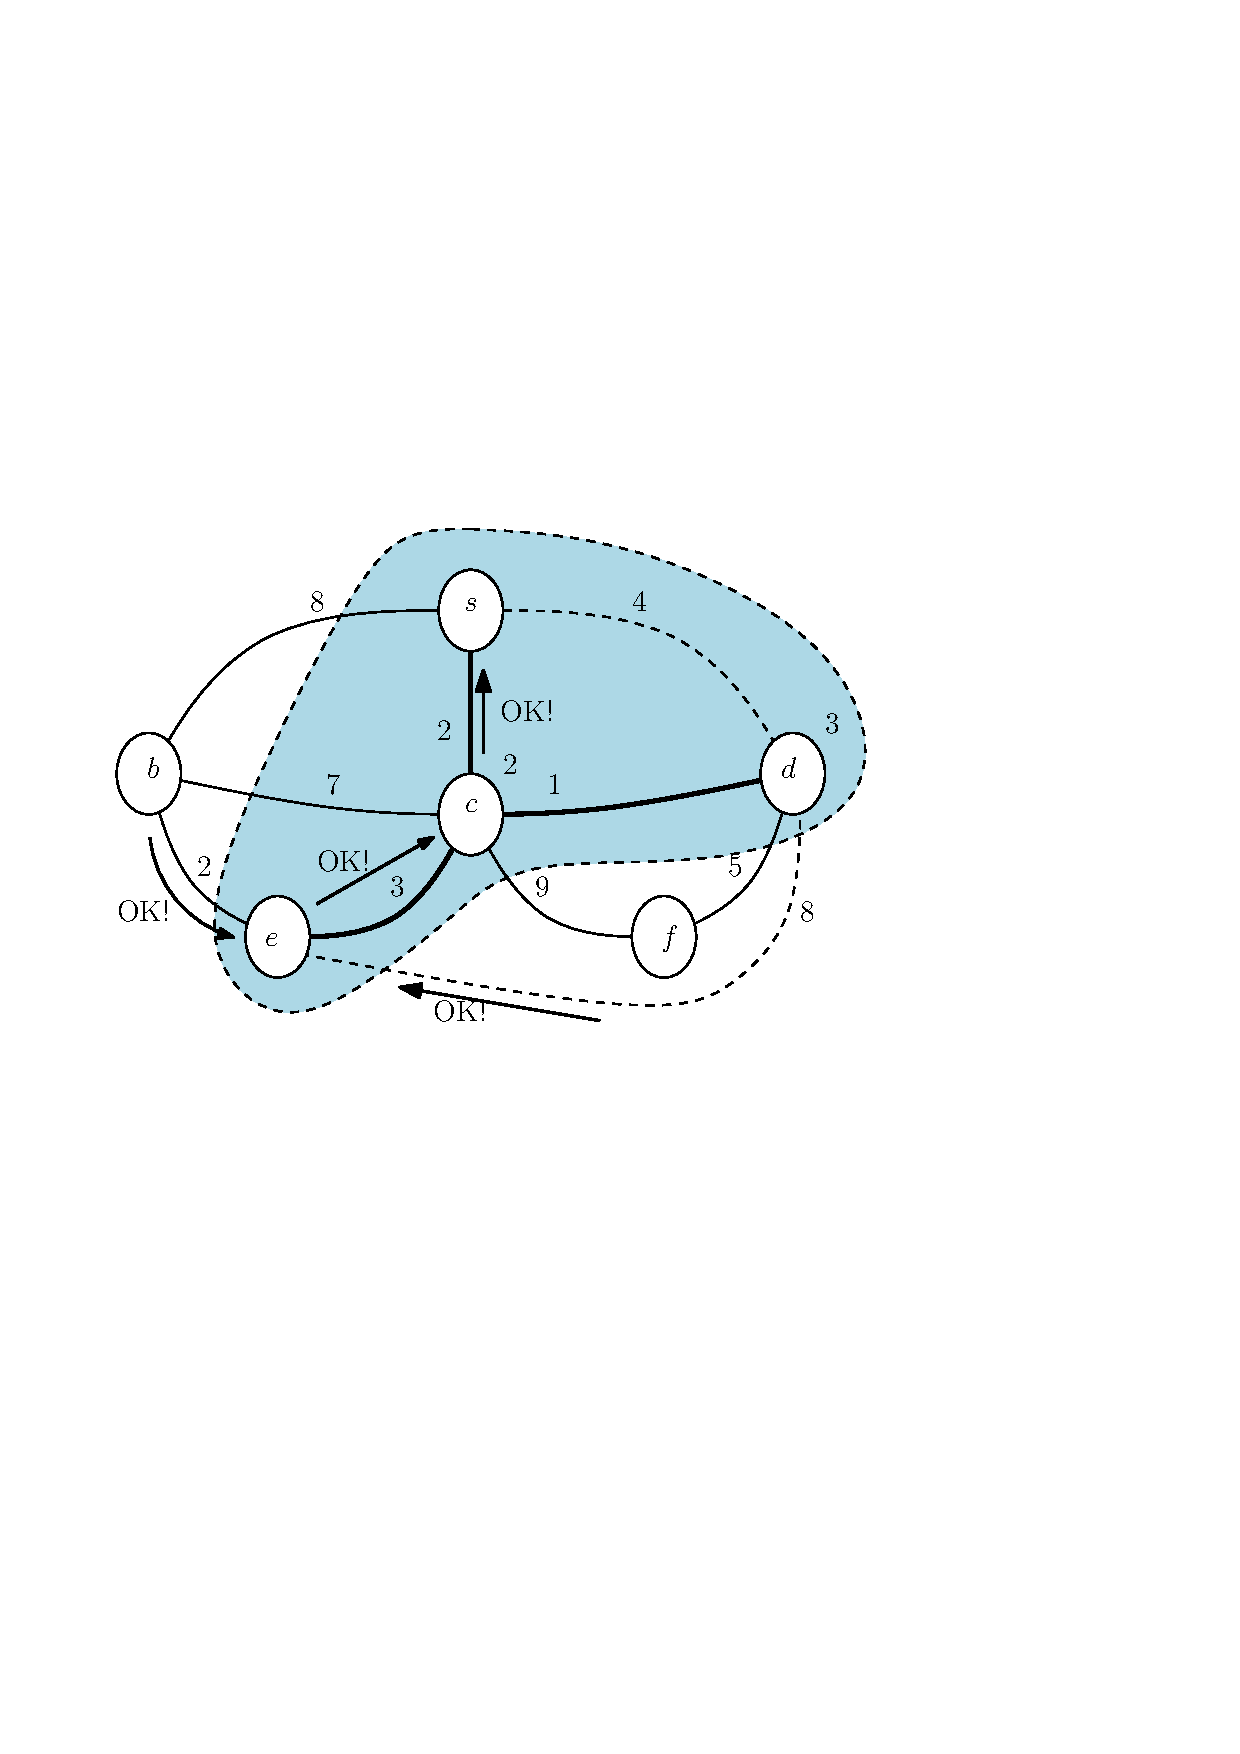
\includegraphics[scale=0.6]{PT6.pdf}
	\end{figure}
\end{frame}

\begin{frame}
	\frametitle{PT-Construction: Recap}

	Ogni nodo nell'albero conosce il suo \textbf{costo}\\
	(cammino minimo verso la radice).

	\begin{block}{Pseudocodice}
	\begin{itemize}
		\item (\textcolor{red}{start}) La radice diffonde in $T$ l'inizio di una nuova iterazione.
		\item Ogni nodo in $T$ calcola localmente la distanza più breve 
			\textit{dalla radice ai vicini di T}.
		\item 	(\textcolor{red}{minimum}) Il minimo globale è calcolato alla radice, e il link corrispondente
			è scelto.
		\item 	(\textcolor{red}{expansion}) La radice notifica il corrispondente nodo della scelta.
		\item 	(\textcolor{red}{neighbour notification}) Il nodo notificato informa i suoi vicini in modo che si possano formare
			i nuovi link interni.
		\item 	(\textcolor{red}{notification}) Dopo aver ricevuto gli acknoledgement, il nodo notificato
			informa la radice della terminazione dell'iterazione. 
	\end{itemize}
	\end{block}
\end{frame}

\begin{frame}
	\frametitle{Complessità di PT-Construction}
	
	Start, minimum, expansion, notification:
	\\Sia $n_i$ il numero di nodi nell'albero al passo $i$
	$$\sum_{i=1}^{n-1}\left( \left( 4n_i-1 \right)+2 \right)=2n^2-4n+1=O(n^2)$$
	\vfill

	\pause
	Neighbour notification:
	$$2\sum_{x\in V} |N(x)|=2\sum_{x\in V}d(x)=4m=O(m)$$
	\vfill

	\pause
	Broadcast di terminazione locale: $n-1$
	\vfill

	Totale: $O(m+n^2)=O(n^2)$\\
	\pause
	\textcolor{red}{Warning!} si tratta del costo della tabella di routing di un solo nodo!
\end{frame}

\begin{frame}
	\frametitle{All-Pairs Shortest Path}
	
	\begin{figure}[h]
	\centering
	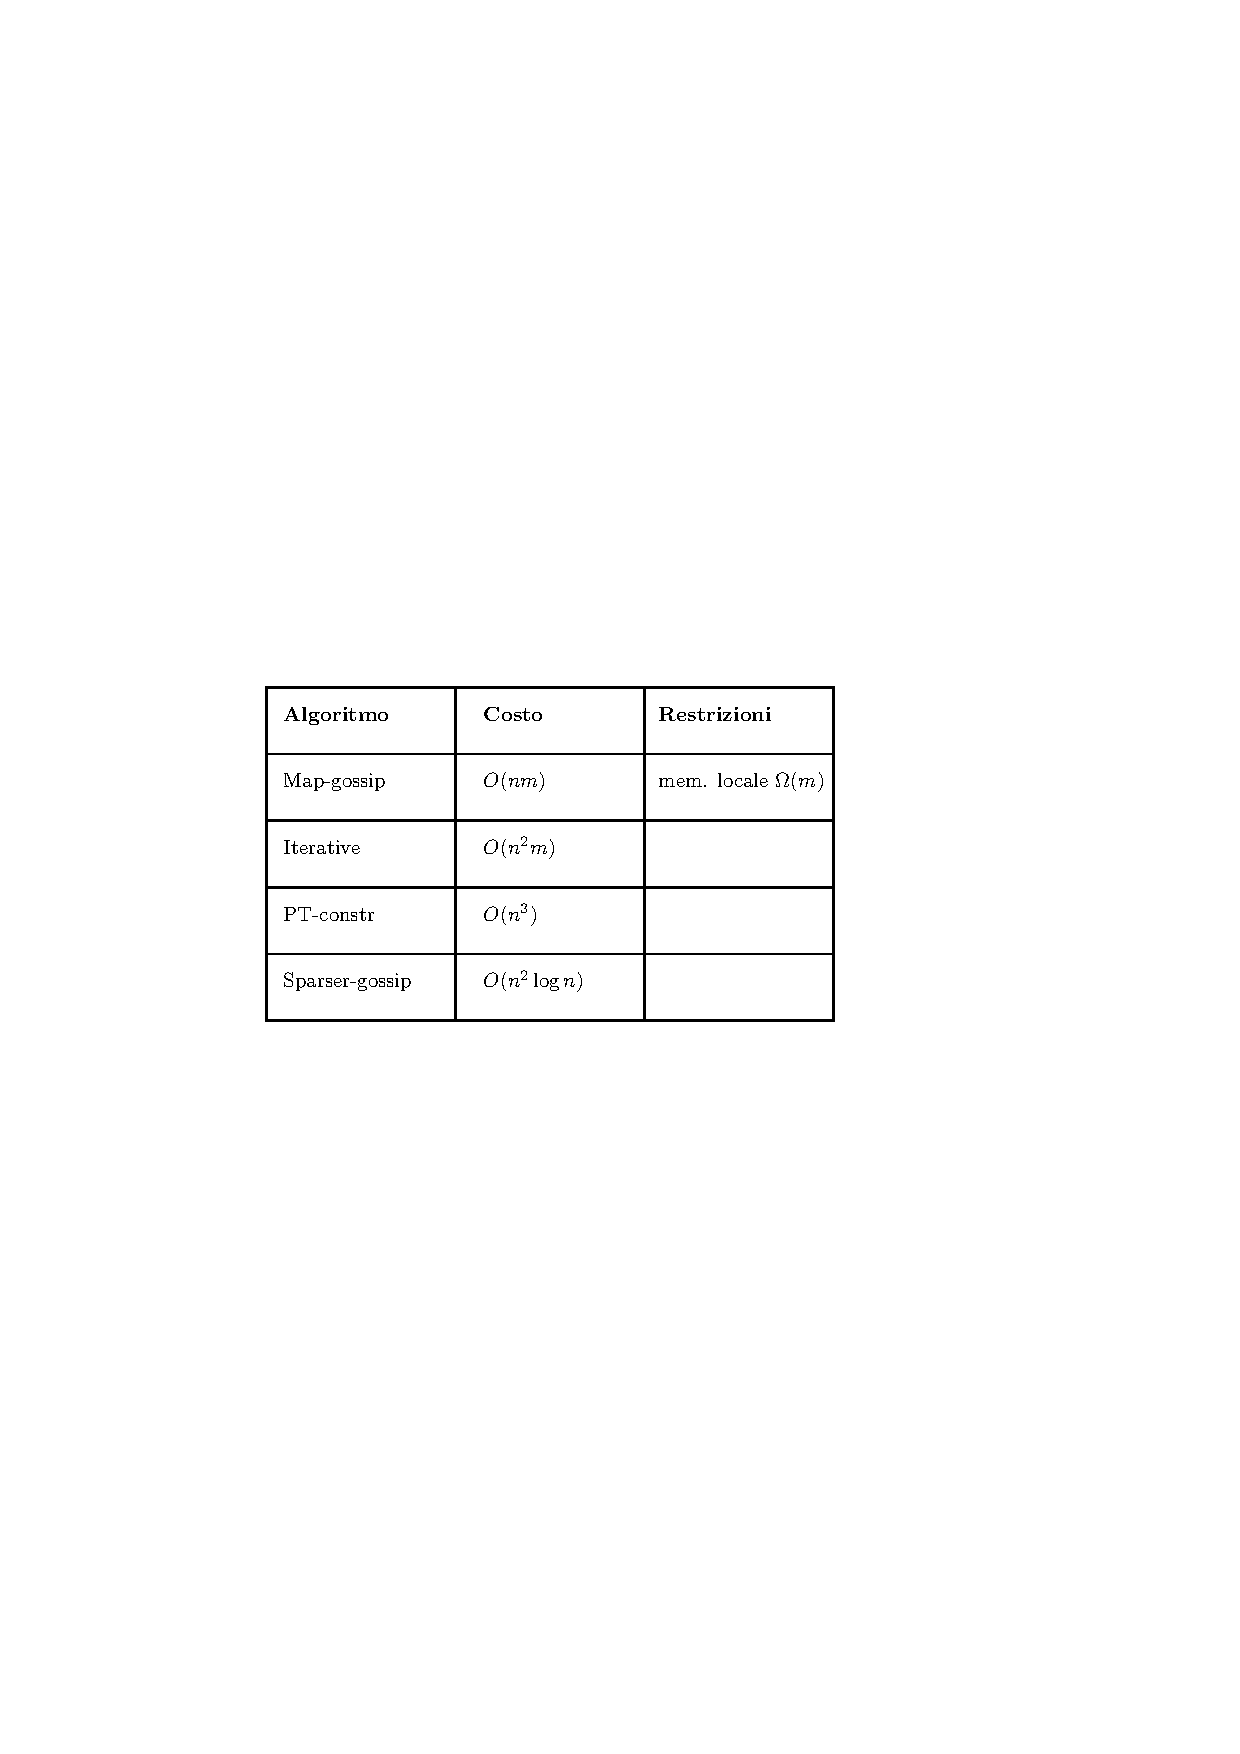
\includegraphics[scale=1]{results_table.pdf}
	\end{figure}
\end{frame}
\end{document}
